
%% 
%% Copyright 2007-2020 Elsevier Ltd
%% 
%% This file is part of the 'Elsarticle Bundle'.
%% ---------------------------------------------
%%




%% It may be distributed under the conditions of the LaTeX Project Public
%% License, either version 1.2 of this license or (at your option) any
%% later version.  The latest version of this license is in
%%    http://www.latex-project.org/lppl.txt
%% and version 1.2 or later is part of all distributions of LaTeX
%% version 1999/12/01 or later.
%% 
%% The list of all files belonging to the 'Elsarticle Bundle' is
%% given in the file `manifest.txt'.
%% 

%% Template article for Elsevier's document class `elsarticle'
%% with numbered style bibliographic references
%% SP 2008/03/01
%%
%% 
%%
%% $Id: elsarticle-template-num.tex 190 2020-11-23 11:12:32Z rishi $
%%
%%
\PassOptionsToPackage{dvipsnames}{xcolor}
% \documentclass[authoryear,preprint,12pt]{elsarticle}
% \documentclass[numbers,webpdf]{ima-authoring-template}%
% \documentclass[a4paper,fleqn]{cas-sc}

%% Use the option review to obtain double line spacing
% \documentclass[preprint,12pt]{elsarticle}

%% Use the options 1p,twocolumn; 3p; 3p,twocolumn; 5p; or 5p,twocolumn
%% for a journal layout:
%% \documentclass[final,1p,times]{elsarticle}
% \documentclass[authoryear,final,1p,times,twocolumn]{elsarticle}
% \documentclass[final,3p,times]{elsarticle}
% \documentclass[authoryear,final,3p,times,twocolumn]{elsarticle}
% \documentclass[final,5p,times]{elsarticle}
\documentclass[final,5p,times,twocolumn]{elsarticle}
\setkeys{Gin}{draft}

%% For including figures, graphicx.sty has been loaded in
%% elsarticle.cls. If you prefer to use the old commands
%% please give \usepackage{epsfig}

% --- Core color support ---
\usepackage{xcolor}
\usepackage{colortbl}

% \usepackage[style=authoryear, maxcitenames=1]{biblatex}
% \usepackage[authoryear]{natbib}

% --- Math ---
\usepackage{amsmath,amssymb,amsfonts,mathtools}
\usepackage{amsthm}

% --- Graphics & Tables ---
\usepackage{graphicx}
\usepackage{caption}
\usepackage{subcaption}
\usepackage{tikz}
\usetikzlibrary{arrows,arrows.meta,positioning,calc,shapes.geometric,fit,backgrounds}
\usepackage{booktabs}
\usepackage{multirow}
\usepackage{makecell}
\usepackage{array}
\usepackage{tabularx}
\usepackage{arydshln}
\usepackage{textcomp}


\usepackage{hhline}

\providecommand{\textproc}[1]{%
  \ifmmode
    \text{\textsc{\detokenize{#1}}}%
  \else
    \textsc{\detokenize{#1}}%
  \fi
}

% These commands accept identifiers containing raw underscores,
% both in text mode and math mode.
\DeclareRobustCommand{\code}[1]{%
  \ifmmode
    \text{\normalfont\ttfamily\detokenize{#1}}%
  \else
    {\normalfont\ttfamily\detokenize{#1}}%
  \fi
}

\DeclareRobustCommand{\edge}[1]{\code{#1}}
\DeclareRobustCommand{\node}[1]{\code{#1}}

\usepackage{algorithm}
\usepackage[noend]{algpseudocode}

\floatname{algorithm}{Algorithm}

\captionsetup[algorithm]{
  font=small,
  labelfont=bf,
  labelsep=period,
  justification=raggedright,
  singlelinecheck=false,
  skip=4pt
}

\algrenewcommand\algorithmicrequire{\textbf{Input:}}
\algrenewcommand\algorithmicensure{\textbf{Output:}}

\algrenewcommand\algorithmiccomment[1]{%
  \hfill$\triangleright$\,\textit{#1}%
}

\algrenewcommand\alglinenumber[1]{%
  \scriptsize\color{gray!75!black}#1%
}

\algnewcommand{\Stage}[1]{%
  \Statex\vspace{1pt}%
  \textbf{#1}%
  \vspace{1pt}%
}

\algnewcommand{\Continue}{%
  \State \textbf{continue}%
}

\AtBeginDocument{%
  \providecommand{\algorithmautorefname}{Algorithm}%
  \renewcommand{\algorithmautorefname}{Algorithm}%
}

% --- Floats ---
\usepackage{float}
\usepackage{placeins}
\usepackage{stfloats}

% --- Boxes ---
\usepackage[most]{tcolorbox}
\usepackage[framemethod=TikZ]{mdframed}

% --- Listings ---
\usepackage{listings}

% --- URLs / refs ---
\usepackage{xurl}

% --- Hyperref LAST ---
\usepackage[colorlinks=true,
    linkcolor=MidnightBlue,
    citecolor=ForestGreen,
    urlcolor=BrickRed
]{hyperref}

\usepackage{pifont}
\newcommand{\cmark}{\textcolor{green!60!black}{\ding{51}}}
\newcommand{\xmark}{\textcolor{red}{\ding{55}}}

% --- Theorems ---
\newtheorem{theorem}{Theorem}
\newtheorem{assumption}{Assumption}
\newtheorem*{proofsketch}{Proof Sketch}
\theoremstyle{plain}

% --- Custom colors ---
\definecolor{titlegray}{HTML}{555555}
\definecolor{framegray}{gray}{0.6}
\definecolor{lightgray}{gray}{0.97}


% --- Diff listings ---
\lstdefinelanguage{diff}{
  morecomment=[f][\color{gray}]{@@},
  morecomment=[f][\color{gray}]{---},
  morecomment=[f][\color{gray}]{+++},
  morecomment=[f][\color{red}]{-},
  morecomment=[f][\color{green!60!black}]{+},
}
\lstdefinestyle{diff}{
  language=diff,
  basicstyle=\ttfamily\footnotesize,
  columns=fullflexible,
  keepspaces=true,
  showstringspaces=false,
  breaklines=true
}
\definecolor{deepblue}{RGB}{0, 0, 139}
% Positive deltas in the RQ4 tables; dark enough to stay legible in greyscale print.
\definecolor{gainGreen}{RGB}{0, 120, 60}

% --- Cypher (Neo4j query language) listing style ---
\definecolor{cybg}{gray}{0.965}
\definecolor{cykw}{rgb}{0.13,0.13,0.62}
\definecolor{cycm}{rgb}{0.40,0.55,0.40}

\lstdefinelanguage{Cypher}{
  morekeywords={
    MATCH,OPTIONAL,MERGE,CREATE,DELETE,DETACH,SET,REMOVE,RETURN,WITH,
    WHERE,UNWIND,CALL,YIELD,IN,TRANSACTIONS,OF,ROWS,AS,ON,ORDER,BY,
    LIMIT,SKIP,COLLECT,DISTINCT,CONSTRAINT,INDEX,FOR,REQUIRE,IS,
    UNIQUE,AND,OR,NOT,CONTAINS,count,coalesce,labels,type,head,size,
    toLower
  },
  sensitive=false,
  morecomment=[l]{//},
  morestring=[b]"
}

\lstdefinestyle{cypher}{
  language=Cypher,
  backgroundcolor=\color{cybg},
  basicstyle=\ttfamily\scriptsize,
  keywordstyle=\color{cykw}\bfseries,
  commentstyle=\color{cycm}\itshape,
  breaklines=true,
  columns=fullflexible,
  keepspaces=true,
  showstringspaces=false,
  frame=single,
  framerule=0.3pt,
  xleftmargin=3pt,
  xrightmargin=2pt,
  aboveskip=4pt,
  belowskip=4pt
}

% Listing caption and reference names
\renewcommand{\lstlistingname}{Cypher Query}
\renewcommand{\lstlistlistingname}{List of Cypher Queries}
\def\lstlistingautorefname{Cypher Query}

\newtcolorbox{boxnote}{
  colback=white,
  boxrule=0.4pt,
  borderline west={2pt}{0pt}{black!60},
}

\renewcommand{\sectionautorefname}{Section}
\renewcommand{\subsectionautorefname}{Section}
\renewcommand{\subsubsectionautorefname}{Section}
\providecommand{\algorithmautorefname}{Algorithm}
% elsarticle already includes "Appendix" in appendix section numbers
\AtBeginDocument{%
  \def\appendixautorefname{}%
}

\tikzset{
  ast/.style={
    circle,
    draw=black!60,
    fill=white,
    line width=0.8pt,
    minimum size=25mm,
    inner sep=2pt,
    align=center,
    font=\small\sffamily
  }
}

\tikzset{
  ast root/.style={
    ast,
    minimum size=34mm,
    font=\normalsize\sffamily,
    fill=blue!2,
    draw=blue!25!black
  }
}

\tikzset{
  basic type ast/.style={
    ast,
    fill=black!1,
    draw=black!50
  }
}

\tikzset{
  identifier ast/.style={
    ast,
    fill=brown!2,
    draw=brown!25!black
  }
}

\tikzset{
  parameter ast/.style={
    ast,
    fill=blue!2,
    draw=blue!20!black
  }
}

\tikzset{
  return ast/.style={
    ast,
    fill=violet!2,
    draw=violet!20!black
  }
}

\tikzset{
  binaryop ast/.style={
    ast,
    fill=brown!2,
    draw=brown!20!black
  }
}

\tikzset{
  file/.style={
    rectangle,
    rounded corners=3mm,
    draw=green!35!black,
    fill=green!4,
    line width=0.8pt,
    minimum width=31mm,
    minimum height=16mm,
    align=center,
    font=\normalsize\sffamily
  }
}

\tikzset{
  relation/.style={
    -{Latex[length=2.8mm,width=2mm]},
    draw=black!70,
    line width=0.85pt,
    line cap=round
  }
}

\tikzset{
  edge label/.style={
    fill=white,
    inner xsep=3pt,
    inner ysep=1.5pt,
    align=center,
    font=\small\sffamily\bfseries,
    text depth=0pt
  }
}

\newcommand{\idbox}[1]{%
  \begingroup
  \setlength{\fboxsep}{3pt}%
  \setlength{\fboxrule}{0.7pt}%
  \fbox{\strut #1}%
  \endgroup
}

\tikzset{
  commit node/.style={
    rectangle,
    rounded corners=3mm,
    draw=black,
    fill=white,
    line width=0.9pt,
    minimum width=35mm,
    minimum height=17mm,
    align=center,
    font=\sffamily\large
  }
}

\tikzset{
  file node/.style={
    rectangle,
    rounded corners=3mm,
    draw=black,
    fill=white,
    line width=0.9pt,
    minimum width=31mm,
    minimum height=15mm,
    align=center,
    font=\sffamily\large
  }
}

\tikzset{
  developer node/.style={
    circle,
    draw=black,
    fill=white,
    line width=0.9pt,
    minimum size=25mm,
    align=center,
    font=\sffamily\large
  }
}

\tikzset{
  issue node/.style={
    diamond,
    aspect=1.25,
    draw=black,
    fill=white,
    line width=0.9pt,
    minimum width=27mm,
    minimum height=19mm,
    align=center,
    inner sep=1pt,
    font=\sffamily\large
  }
}

\tikzset{
  relation/.style={
    -{Latex[length=3mm,width=2.2mm]},
    draw=black,
    line width=1pt,
    line cap=round
  }
}

\tikzset{
  relation label/.style={
    fill=white,
    inner xsep=3pt,
    inner ysep=1.5pt,
    align=center,
    font=\sffamily\bfseries\normalsize
  }
}
\usepackage{graphicx}
\usepackage{tikz}

\usetikzlibrary{
  arrows.meta,
  calc,
  fit,
  positioning,
  backgrounds
}

\definecolor{deltaAddC}{RGB}{0,140,0}
\definecolor{deltaRemC}{RGB}{190,0,0}
\definecolor{deltaUpdC}{RGB}{230,120,0}
\definecolor{deltaMovC}{RGB}{110,50,180}

\tikzset{
  deltaAst/.style={
    circle,
    draw=black,
    fill=white,
    line width=0.8pt,
    minimum size=8.8mm,
    inner sep=1pt,
    align=center,
    font=\scriptsize\sffamily
  }
}

\tikzset{
  deltaRoot/.style={
    deltaAst,
    minimum size=10mm
  }
}

\tikzset{
  deltaCommit/.style={
    rectangle,
    rounded corners=2mm,
    draw=black,
    fill=white,
    line width=0.8pt,
    minimum width=17mm,
    minimum height=9mm,
    align=center,
    font=\scriptsize\sffamily
  }
}

\tikzset{
  deltaEdge/.style={
    -{Latex[length=1.8mm,width=1.35mm]},
    draw=black,
    line width=0.75pt
  }
}

\tikzset{
  deltaUpdated/.style={
    deltaAst,
    draw=deltaUpdC,
    line width=1.1pt
  }
}

\tikzset{
  deltaRemoveBox/.style={
    draw=deltaRemC,
    dashed,
    rounded corners=1.5mm,
    line width=0.9pt,
    inner sep=2pt,
    fill=deltaRemC,
    fill opacity=0.12
  }
}

\tikzset{
  deltaAddBox/.style={
    draw=deltaAddC,
    dashed,
    rounded corners=1.5mm,
    line width=0.9pt,
    inner sep=2pt,
    fill=deltaAddC,
    fill opacity=0.12
  }
}

\tikzset{
  deltaMoveBox/.style={
    draw=deltaMovC,
    dashed,
    rounded corners=1.5mm,
    line width=0.9pt,
    inner sep=2pt,
    fill=deltaMovC,
    fill opacity=0.12
  }
}

\tikzset{
  deltaTopLabel/.style={
    fill=white,
    inner sep=0.7pt,
    font=\scriptsize\sffamily\bfseries
  }
}

\tikzset{
  deltaSideTitle/.style={
    font=\small\sffamily\bfseries
  }
}

\tikzset{
  deltaRelationLabel/.style={
    fill=white,
    inner sep=1pt,
    font=\scriptsize\sffamily\bfseries
  }
}

\tikzset{
  deltaLegend/.style={
    rectangle,
    rounded corners=1.3mm,
    draw=black!50,
    dashed,
    inner xsep=3pt,
    inner ysep=2pt,
    align=center,
    font=\scriptsize\sffamily
  }
}

\tikzset{
  deltaTreePanel/.style={
    rounded corners=2mm,
    draw=black!12,
    fill=black!3,
    fill opacity=0.5,
    line width=0.5pt
  }
}

\journal{Knowledge-based Systems}

\begin{document}

\begin{frontmatter}

%% Title, authors and addresses

%% use the tnoteref command within \title for footnotes;
%% use the tnotetext command for theassociated footnote;
%% use the fnref command within \author or \address for footnotes;
%% use the fntext command for theassociated footnote;
%% use the corref command within \author for corresponding author footnotes;
%% use the cortext command for theassociated footnote;
%% use the ead command for the email address,
%% and the form \ead[url] for the home page:
%% \title{Title\tnoteref{label1}}
%% \tnotetext[label1]{}
%% \author{Name\corref{cor1}\fnref{label2}}
%% \ead{email address}
%% \ead[url]{home page}
%% \fntext[label2]{}
%% \cortext[cor1]{}
%% \affiliation{organization={},
%%             addressline={},
%%             city={},
%%             postcode={},
%%             state={},
%%             country={}}
%% \fntext[label3]{}

\title{KG-Commit: A Real-Time Knowledge Graph for Just-in-Time Software Defect Prediction}

%% use optional labels to link authors explicitly to addresses:
%% \author[label1,label2]{}
%% \affiliation[label1]{organization={},
%%             addressline={},
%%             city={},
%%             postcode={},
%%             state={},
%%             country={}}
%%
%% \affiliation[label2]{organization={},
%%             addressline={},
%%             city={},
%%             postcode={},
%%             state={},
%%             country={}}

\author[mce]{Mohsen Hesamolhokama}
\ead{hokama@ce.sharif.edu}

\author[mce]{Mohammad Sina Beyrami Aghbash}
\ead{sina.beirami@sharif.edu}

\author[math]{Behnam Rohani}
\ead{behnam.rohani058@sharif.edu}

\author[mce]{Mohammadamin Fazli}
\ead{fazli@sharif.edu}

\author[mce]{Jafar Habibi}
\ead{jhabibi@sharif.edu}

\address[mce]{Department of Computer Engineering, Sharif University of Technology, Tehran, Iran}
\address[math]{Department of Mathematical Sciences, Sharif University of Technology, Tehran, Iran}

% \cortext[cor1]{Corresponding author.}
% \fntext[fn1]{Authors Mohsen Hesamolhokama and Behnam Rohani contributed equally to this work.}

\begin{abstract}
Just-in-time software defect prediction (JIT-SDP) flags a commit as risky the moment it is authored. This need for speed has led most existing approaches to rely on features from the current commit, such as change metrics, commit messages, and code diffs. However, these features provide little information about the repository context in which the change occurs. However, reconstructing such context for every new commit is too costly for continuous integration. We introduce KG-Commit, which is, to the best of our knowledge, the first real-time knowledge graph designed for JIT-SDP. KG-Commit maintains the evolving repository incrementally in Neo4j. Each commit updates only the affected part of the graph, while bounded Cypher queries retrieve the required context at prediction time. This distributes the cost of constructing project context over the lifetime of the repository rather than paying it again for every prediction. KG-Commit combines project-evolution information, including commits, developers, files, and issues, with program structure and the semantics of commit messages and code changes. Its structural layer preserves persistent abstract syntax tree (AST) identities and records only additions, removals, updates, and moves. Storage and maintenance costs therefore depend on the size of the syntactic change rather than on repeated full-tree snapshots. Across [N] projects and [M] commits, KG-Commit improves [PRIMARY METRIC] by [XX\%] over the strongest baseline, achieves a median prediction latency of [X ms], and reduces [STORAGE OR UPDATE COST] by [YY\%]. These results show that rich project context can be incorporated into defect prediction without sacrificing the speed required in a JIT setting.

\end{abstract}

% Use if graphical abstract is present
% \begin{graphicalabstract}
% \includegraphics{figs/grabs.pdf}
% \end{graphicalabstract}

\begin{keyword}
%% keywords here, in the form: keyword \sep keyword
%% PACS codes here, in the form: \PACS code \sep code
%% MSC codes here, in the form: \MSC code \sep code
%% or \MSC[2008] code \sep code (2000 is the default)
Knowledge Graphs \sep JIT \sep SDP \sep Commit-level Analysis \sep Real-time Project Evolution
\end{keyword}

\end{frontmatter}

\begin{abstract}

\end{abstract}

% Use if graphical abstract is present
% \begin{graphicalabstract}
% \includegraphics{figs/grabs.pdf}
% \end{graphicalabstract}

\section{Introduction}
\label{sec:introduction}

Software now sits behind almost every product and service that people rely on, and a single faulty change can bring down a critical system or reach millions of users within minutes. Software quality is therefore a constant concern for development teams, yet the effort available for testing and code review is always limited. Software defect prediction (SDP) helps teams direct that effort to the right place by estimating which parts of a system are most likely to be faulty~\cite{menzies2007data,lessmann2008benchmarking,hall2012systematic}. Classical SDP models work at the level of files, modules, or
releases~\cite{wang2016automatically,li2017software,zhou2022software}. Predictions at this granularity arrive late in the development cycle, after many changes have accumulated, when the specific change that introduced a defect is hard to trace and recall. Just-in-time defect prediction (JIT-SDP) was introduced to close this gap~\cite{mockus2000predicting,kamei2013large}. It evaluates each change, that is, each commit, as soon as it is submitted, so a
risky change can be reviewed while its author still remembers the context. Because of this fine granularity and this immediate feedback, JIT-SDP has become a natural fit for continuous integration and an active research topic~\cite{zhao2023systematic}.

For more than a decade, the workhorse of JIT-SDP has been a compact set of hand-crafted metrics that summarize each commit. These metrics describe the size of the change, the amount of code churn~\cite{nagappan2005use}, how widely the change spreads across files and subsystems, and the experience of the author~\cite{kamei2013large,mcintosh2018fix}. They are then passed to standard classifiers. As deep learning matured, the field moved from describing commits with metrics toward learning features from the change itself. Yang et al. turned the metric set into richer features with a deep belief network~\cite{yang2015deep}. DeepJIT and CC2Vec learn representations from the commit message and the code diff~\cite{hoang2019deepjit,hoang2020cc2vec}. Later models added line-level localization~\cite{pornprasit2021jitline,pornprasit2023deeplinedp}, brought in pre-trained code encoders such as CodeBERT~\cite{ni2022best,jiang2025bicc}, and explored parameter-efficient tuning of such encoders~\cite{abutalib2024parameter}. For all their differences, these models share a blind spot. They represent a commit as a vector of summary numbers or as a flat sequence of tokens, and they barely use the relational structure of the code or of the wider project in which the change lives~\cite{bryan2023graph,zhao2023systematic}.

What these models leave on the table is the broader project structure. A knowledge graph captures exactly this kind of structure, since it stores information as entities and as typed relations among them~\cite{hogan2021knowledge,ji2022survey} and supports reasoning and learning over it~\cite{nickel2016review}. Knowledge graphs have reshaped recommendation, the life sciences, and security~\cite{wang2019kgat,maclean2021knowledge,zhao2024survey}. Their adoption in software engineering, however, is recent and narrow, and it is largely confined to organizing artifacts such as APIs and libraries~\cite{liu2023recommending}. Their use in software defect prediction is scarcer still, and in the just-in-time setting it is, to the best of our knowledge, absent. The opportunity is large because a commit is relational by nature. It edits particular files and functions, it depends on other parts of the system, it has an author, and it carries an intent that is stated in its message. The opportunity grows further with real-time knowledge graphs, which are also called temporal or dynamic knowledge graphs~\cite{zhang2024survey,cai2024survey}. These graphs absorb new events as they happen and keep an up-to-date view of an evolving
domain~\cite{trivedi2017knowevolve,goel2020diachronic}. Software grows one commit at a time, which makes it an almost ideal subject for a graph that is maintained incrementally.

In just-in-time prediction, however, accuracy is of little value if it arrives too late~\cite{kamei2013large}. A prediction is useful only at the instant the commit is created, so the model must respond at a low computational cost. This requirement creates a tension that the field has not resolved. Project-level context, such as how a changed function is called elsewhere or how a file depends on others, is known to improve defect prediction~\cite{zimmermann2009cross,nam2013transfer}, but recomputing it from scratch for every commit is expensive. To stay fast, many methods sidestep this context and predict from the commit text alone, which keeps the features cheap but shallow~\cite{hoang2019deepjit,hoang2020cc2vec,pornprasit2021jitline}, and some reduce the model to a single low-cost feature~\cite{zeng2021deep} or to lightweight retrieval over past commits~\cite{sahar2024irjit}. The open question is whether a feature can carry rich project-specific context and still be cheap to obtain at prediction time. Real-time knowledge graphs offer a direct answer, and they align unusually well with the just-in-time setting. The idea is to amortize the cost of context over the lifetime of the project. The graph is updated at each commit, and every update is cheap because it touches only a local region of the graph~\cite{zhao2023incremental}. When a later commit with an unknown label arrives, the context that it needs already exists in the graph, and a graph query language such as Cypher can read that context with a small and bounded cost~\cite{francis2018cypher,angles2017foundations}. In this way the heavy work is paid gradually as the project grows, and only light work is left for the moment of prediction, which is exactly when speed matters most.

Building on this insight, we introduce KG-Commit, a real-time knowledge graph that evolves with the repository and provides project-specific context when each commit arrives. KG-Commit is maintained incrementally in Neo4j, where each new commit updates only the affected part of the graph and prediction-time information is retrieved through bounded Cypher queries. Its representation consists of three layers. The Core layer captures repository evolution through commits, developers, files, issues, and their relations. The Structural layer represents within-file program structure using abstract syntax trees and maintains this structure through delta extraction rather than storing a complete snapshot for every revision. It preserves persistent node identities and records only additions, removals, updates, and moves. The Commit Semantic-Text Graph layer represents the semantics of commit messages and diff text using graph-of-words statistics, term associations, change intents, and propagated defect-risk signals. Commits are processed chronologically, and only information available at prediction time is used. KG-Commit is analyzed using complementary graph-based and feature-based inference methods, whose outputs are combined to estimate the defect risk of each incoming commit. We evaluate the framework in terms of predictive performance, query cost, update cost, and suitability for online just-in-time prediction.

\subsection{Motivating Example}
\label{sec:motivating}

Consider a commit that only changes the location of a file, for example by moving \texttt{config.py} from the \texttt{utils/} package to the \texttt{core/} package (\autoref{fig:motivating}). Judged on its own, the commit looks harmless. It moves a file without changing its contents, so its change metrics are small and nothing inside the change points to a defect. A developer reviewing the commit, and a model that reads only the commit, would both consider it clean~\cite{hoang2019deepjit,zeng2021deep}. The commit is nonetheless bug-inducing, because another part of the project still refers to the file through its old path. The file \texttt{api/server.py}, which this commit does not touch, still contains \texttt{from utils.config import Config}, so after the move this import points to a file that no longer exists and the program breaks at a location far from the commit.

The defect cannot be detected from the commit in isolation. It becomes visible only when the rest of the project is taken into account. Reliably labeling such a commit therefore requires information about the project context that surrounds the change, and not only the content of the change itself.

\begin{figure*}[t]
\centering
\includegraphics[width=0.92\linewidth]{kg_commit_motivating_example.pdf}
\caption{A commit moves \texttt{config.py} from \texttt{utils/} to
\texttt{core/}. The change has no effect inside the file, so it looks clean, but
\texttt{api/server.py} elsewhere in the project still imports the old path and
fails at runtime. The defect is not visible from the commit alone.}
\label{fig:motivating}
\end{figure*}

\subsection{Contributions}
The main contributions of this paper are as follows: 

\begin{itemize}

\item \textbf{A real-time solution to the context--speed trade-off in JIT-SDP.} To the best of our knowledge, KG-Commit is the first approach to provide rich project context without sacrificing the speed required for JIT prediction. It achieves this by maintaining context in a graph database and retrieving it through low-cost queries.

\item \textbf{A layered design for KG-Commit with AST-delta maintenance.} We design a three-layer representation, containing (1) high-level repository relations, (2) code structure, and (3) commit semantics. Its AST delta-extraction method maintains each file’s evolving structure without storing a complete AST for every revision.

\item \textbf{A broad online evaluation across diverse knowledge-graph inference methods.}
We evaluate KG-Commit on [X] Apache projects across multiple inference methods, representation choices, and JIT-SDP baselines. The results demonstrate improved predictive performance while retaining the efficiency required for real-time use.

\end{itemize}

\subsection{Paper Outline}
The remainder of this paper is organized as follows. Section 2 reviews related work on JIT-SDP, code representation for defect prediction, and knowledge graphs in software engineering. Section 3 presents KG-Commit, including its online formulation, multilayer knowledge-graph representation, incremental maintenance, and inference methods. Section 4 describes the research questions, dataset, baselines, experimental protocol, settings, and evaluation metrics. Section 5 reports the results on predictive performance, efficiency and scalability, representation choices, and inference methods. Section 6 discusses the online evaluation setting, parameter sensitivity, component contributions, long-term graph growth, and limitations. Finally, Section 7 concludes the paper.


\section{Related Work}
\label{sec:related_work}

Our work brings together three research lines: JIT-SDP, the representation of source code for defect prediction, and knowledge graphs. We review each line in turn and close by positioning our proposal, which represents the sequence of code changes as a real-time knowledge graph and queries that graph to predict defects.

\subsection{Just-in-Time Software Defect Prediction}
\label{subsec:jitsdp}

Traditional defect prediction works at coarse levels such as the file, the module, or the release \cite{Menzies2010}. This delays feedback and forces developers to inspect large amounts of code. JIT-SDP instead targets the individual change, that is, the commit, so that risky changes can be reviewed as soon as they are submitted. The idea goes back to the change-level risk models of Mockus and Weiss~\cite{mockus2000predicting}, and its modern formulation was established by the large-scale empirical study of Kamei et al.~\cite{kamei2013large}. That study introduced a set of change-level metrics that is now standard, covering the size, the diffusion, the history, and the developer experience of a change, together with effort-aware evaluation that ranks changes by defect likelihood per unit of inspection effort. The labels these models rely on usually come from the SZZ algorithm, which links a fix to the change that induced it~\cite{sliwerski2005changes}, and an early formulation cast the task as classifying each change as clean or buggy~\cite{kim2008classifying}. Later studies examined how such models generalize across
projects~\cite{fukushima2014empirical,kamei2016studying} and how they degrade over time, with McIntosh and Kamei~\cite{mcintosh2018fix} showing that fix-inducing changes are a moving target.

A first wave of learning-based work moved beyond hand-crafted metrics. Yang et al.~\cite{yang2015deep} used a deep belief network to combine the traditional change features into more expressive ones. End-to-end models soon followed. DeepJIT~\cite{hoang2019deepjit} learns features directly from the commit message and the code change, and CC2Vec~\cite{hoang2020cc2vec} learns representations of code changes guided by their log messages. Other work predicts defects at finer levels, such as the file and the line within a commit~\cite{pascarella2019fine,pornprasit2021jitline}, and complementary efforts explain individual predictions to developers~\cite{pornprasit2021pyexplainer}. Recent models use pre-trained code encoders. JIT-Fine combines semantic features from CodeBERT with expert features in a single model~\cite{ni2022best}, bi-modal pre-training sharpens change semantics~\cite{jiang2025bicc}, and parameter-efficient tuning adapts such encoders at a lower cost~\cite{abutalib2024parameter}. This drive toward complex models has been questioned. Zeng et al.~\cite{zeng2021deep} report that a simple model built on a single churn feature matches much heavier models, Zhou et al.~\cite{zhou2025bridging} argue for combining expert knowledge with deep learning, fusing expert and semantic metrics has been shown to help~\cite{chen2023boosting}, and a lightweight information-retrieval model attains competitive accuracy at high speed~\cite{sahar2024irjit}.

Two practical concerns have received growing attention. The first is the online nature of the task. Commits arrive as a stream, labels become available only after a verification latency, and the class distribution drifts. Cabral and Minku~\cite{cabral2023towards} study reliable online JIT-SDP under these conditions, and Tabassum et al.~\cite{tabassum2023cross} extend the setting to cross-project online learning. The second concern is the structure of the change itself. Recognizing that flat metrics and token sequences discard the relational structure of code, Bryan and Moriano~\cite{bryan2023graph} build contribution graphs over developers and files and obtain large gains over feature-based JIT-SDP. The survey by Zhao et al.~\cite{zhao2023systematic} consolidates this body of work and identifies the modeling of structural and semantic information as an open direction, while methodological studies stress the need for sound model validation~\cite{tantithamthavorn2017empirical}. Our work follows this structural direction, but rather than graphs of developers and files we model the changed code and its project context as a knowledge graph.

\subsection{Software Defect Prediction and Code Representation}
\label{subsec:coderep}
Defect prediction has a long history at the file and module level. Early models learn from static code attributes such as size and complexity metrics~\cite{menzies2007data}, and a parallel line shows that change and process metrics, such as code churn and the complexity of the change history, are often stronger predictors than the code itself~\cite{nagappan2005use,moser2008comparative,hassan2009predicting}. Large empirical studies and benchmarks compare classifiers and datasets under a common protocol~\cite{lessmann2008benchmarking,hall2012systematic,dambros2012evaluating}, and a broad literature studies how to transfer a model from one project to another when local data are scarce~\cite{zimmermann2009cross,nam2013transfer}. These studies establish the metrics, the evaluation practices, and the datasets on which later work builds.

A second line learns representations of code rather than relying on hand-crafted metrics. It is motivated by the observation that software is repetitive and predictable, much like natural language~\cite{hindle2012naturalness}, and it borrows distributed representations from natural language processing~\cite{mikolov2013distributed}. Wang et al.~\cite{wang2016automatically} learn semantic features from token sequences of abstract syntax trees (ASTs) with a deep belief network, and convolutional and tree-based models exploit syntactic structure more directly~\cite{mou2016convolutional,li2017software,tai2015improved}. A widely used family encodes code through AST paths, as in code2vec~\cite{alon2019code2vec} and code2seq~\cite{alon2019code2seq}, while ASTNN encodes statement-level subtrees~\cite{zhang2019astnn}. Self-supervised and pre-trained models have since become a common backbone, including InferCode~\cite{bui2021infercode}, contextual code embeddings from large Transformers~\cite{kanade2020learning}, CodeBERT~\cite{feng2020codebert}, GraphCodeBERT~\cite{guo2021graphcodebert}, CodeT5~\cite{wang2021codet5}, and models that add global relational information to sequence models~\cite{hellendoorn2020global}.

Because trees and token sequences cannot express data and control dependencies, a growing body of work represents programs as graphs and learns over them with graph neural networks~\cite{scarselli2009graph,wu2021comprehensive}. Allamanis et al.~\cite{allamanis2018learning} add data-flow and other edges to ASTs and reason over the result with gated graph neural networks~\cite{li2016gated}, and Devign~\cite{zhou2019devign} composes AST, control-flow, and data-flow information into a single graph for vulnerability identification. In defect prediction, graph-based models combine the semantic content of code with the structure of its dependencies. Zhou et al.~\cite{zhou2022software} model ASTs
together with class-dependency networks, Liu et al.~\cite{liu2023semantic} enrich code-derived semantics with external knowledge, \v{S}iki\'{c} et al.~\cite{sikic2022graph} classify modules with a graph neural network over the AST, and flow-augmented ASTs support related code tasks~\cite{wang2020detecting}. Recent surveys confirm the shift toward deep and structural representations in defect prediction~\cite{zain2023application}. These methods show that structure helps, but they operate mostly within a file or a module, and they do not model the project-wide relations or the just-in-time constraint that our work targets.

\subsection{Knowledge Graphs and Their Applications}
\label{subsec:kg}

Knowledge graphs (KGs) organize information as entities and as the typed relations among them, and they provide a structured basis for reasoning, retrieval, and learning~\cite{hogan2021knowledge,ji2022survey,nickel2016review}. A large body of work embeds KGs into continuous vector spaces so that symbolic facts can be used by machine learning models~\cite{ji2022survey,wang2017knowledge}. Tensor-factorization models such as RESCAL first learned over multi-relational data~\cite{nickel2011three}, translational models such as TransE~\cite{bordes2013translating}, TransH~\cite{wang2014knowledge}, and TransR~\cite{lin2015learning} model relations as geometric operations, and bilinear and complex-valued scorers such as DistMult~\cite{yang2015embedding}, ComplEx~\cite{trouillon2016complex}, and RotatE~\cite{sun2019rotate} increase their expressiveness. Neural scorers such as ConvE~\cite{dettmers2018convolutional} and relational graph convolutional networks~\cite{schlichtkrull2018modeling}, together with composition-based variants~\cite{vashishth2020composition}, bring message passing to multi-relational data.

Knowledge graphs have proven useful across many domains. Large general-purpose graphs such as YAGO, Freebase, and Wikidata showed that web-scale relational knowledge can be curated and queried~\cite{suchanek2007yago,bollacker2008freebase,vrandecic2014wikidata}. In recommendation, they reduce data sparsity and improve explainability, as in KGAT~\cite{wang2019kgat} and RippleNet~\cite{wang2018ripplenet} and the literature surveyed by Guo et al.~\cite{guo2022survey}. In the life sciences they integrate biomedical evidence for drug discovery~\cite{maclean2021knowledge}, in security they consolidate threat intelligence~\cite{zhao2024survey}, and they have been injected into language models to improve understanding~\cite{zhang2019ernie}. A further line models how facts change over time through temporal knowledge graphs~\cite{zhang2024survey,cai2024survey,trivedi2017knowevolve,goel2020diachronic,jin2020renet,lacroix2020tensor}. Within software engineering, knowledge graphs organize artifacts such as APIs and libraries; for example, Liu et al.~\cite{liu2023recommending} recommend analogical APIs by embedding an API knowledge graph. Despite this progress, knowledge graphs have rarely been used to represent the fine-grained structure of a single code change for defect prediction, and their use in the just-in-time setting is, to the best of our knowledge, unexplored.

% \subsection{Summary and Positioning}
% \label{subsec:positioning}
% In summary, JIT-SDP has progressed from engineered change metrics toward learned and increasingly structural representations, yet most models still treat a commit as a bag of metrics or as a token sequence, and only recent work has begun to use graph structure~\cite{bryan2023graph,zhao2023systematic}. Research on defect prediction and code representation shows that graph views of code capture structural information that flat features miss, which benefits tasks from module classification to vulnerability
% detection~\cite{zhou2019devign,zhou2022software,sikic2022graph}. Knowledge graphs, in turn, are a powerful way to encode typed relations and to make them learnable across domains~\cite{hogan2021knowledge,ji2022survey}. Our work brings these threads together. We represent a code change as a knowledge graph that makes its syntactic and semantic relations explicit, and we maintain this graph in real time so that project-level context can be queried cheaply at the moment a commit is submitted. This design targets two gaps highlighted above: the limited use of project-wide relational structure in JIT-SDP, and the absence of knowledge-graph representations of code changes for this task.

\section{Methodology}
\label{sec:methodology}

\subsection{Motivation}
\label{sec:motivation}
JIT-SDP must quickly provide feedback as a change is submitted \cite{kamei2013large}. Existing models therefore rely largely on features extracted from the current commit, such as code diffs and churn metrics \cite{nagappan2005use}, but these features omit broader repository context, including developer history, file co-change patterns, and cross-file dependencies \cite{??,??,??}. The maintenance and efficient integration of such context is a challenging task in a just-in-time setting \cite{??,??,??}. KG-Commit instead maintains it incrementally in Neo4j: each commit updates only the affected graph neighbourhood, so the accumulated project context is available at prediction time through bounded Cypher queries.

\subsection{Problem Formulation}
\label{sec:problem_formulation}

Let a software project $P$ be represented as a chronologically ordered sequence of commits $C = \{c^{(1)}, c^{(2)}, \dots, c^{(n)}\}$. Each commit $c^{(i)} \in C$ represents an evolutionary step that alters the state of the project from $s^{(i-1)}$ to $s^{(i)}$. Each commit $c^{(i)}$ targets a set of pre-existing files $F^{(i)}_{\text{prev}} = \{f_1, f_2, \dots, f_m\}$ and produces a set of modified or newly created files $F^{(i)}_{\text{new}} = \{f'_1, f'_2, \dots, f'_p\}$. Therefore, a commit may add, remove, modify, or rename/move file(s) in the project.

\subsubsection{Defect Modeling}
\label{sec:defect-modeling}
A commit $c^{(i)}$ is defined as bug-inducing if and only if it introduces a defect into the codebase that requires a subsequent fix. Formally, we define the ground-truth binary label $y^{(i)} \in \{0, 1\}$ for any commit starting from index 1 as:

\begin{align}
y^{(i)} = \begin{cases} 1 & \text{if } \exists f \in F^{(i)}_{\text{new}} \text{ such that } f \text{ is defective} \\ 0 & \text{otherwise} \end{cases}
\end{align}

In our experiments, we use the labels provided by the ApacheJIT dataset~\cite{keshavarz2022apachejit}, where bug-inducing commits are identified using an SZZ-style algorithm.
\subsubsection{Operational Constraints}
\label{sec:operational-constraints}
To simulate real-world deployment settings, the online formulation introduces two temporal constraints: a warm-up period $t$ and a gap $g$ \cite{lee2024neurojit,song2023validity}. The warm-up period requires $t$ commits to pass before evaluation begins, restricting the target commit $c^{(j)}$ to indices where $j > t$. The gap $g$ accounts for the operational delay in defect identification (e.g., via the SZZ algorithm), meaning that when commit $c^{(j)}$ arrives, historical ground-truth labels are only resolved and available up to commit $c^{(j-g-1)}$.

\subsubsection{Online Predictive Objective}
\label{sec:online-objective}
Given a target commit $c^{(j)}$ where $j > t$, the objective is to estimate conditional probability $\hat{y}^{(j)}$ that the commit is bug-inducing based on the current project state $s^{(j-1)}$:

\begin{align}
\hat{y}^{(j)} = \hat{\mathbb{P}}\left( y^{(j)} = 1 \;\middle|\; c^{(j)}, s^{(j-1)} \right)
\end{align}

\subsubsection{Knowledge Graph State Representation and Evolution}
\label{sec:kg_evolution}
To avoid recomputing deep repository histories on demand, the abstract project state and its evolutionary history are captured by an incrementally updated knowledge graph $\mathcal{K}^{(j)}$. Upon the arrival of a target commit $c^{(j)}$, its corresponding entities and relations are immediately updated and inserted into the graph before classification occurs. This state evolution follows a recurrence relation defined by a state transition function $\Phi$:

\begin{align}
\mathcal{K}^{(j)} = \Phi\left(\mathcal{K}^{(j-1)}, c^{(j)}, y^{(j-g-1)}\right)
\end{align}

where $c^{(j)}$ provides the immediate modifications for the incoming commit, and $y^{(j-g-1)}$ injects the historical ground-truth label newly exposed by the expiration of the gap window. By unrolling this recurrence, $\mathcal{K}^{(j)}$ preserves the complete history of previous project states and commits:
\begin{align}
\mathcal{K}^{(j)} = \text{Encode}\left( \{s^{(i)}\}_{i=1}^{j}, \; \{c^{(i)}\}_{i=1}^{j}, \; \{y^{(i)}\}_{i=1}^{j-g-1} \right),
\end{align}
in the sense that all this information can later be accessed; in our case, by using the proper Cypher queries on the graph database.

Because $\mathcal{K}^{(j)}$ embeds this entire history alongside the unlabeled properties of the recent commits, the predictive objective is resolved by conditioning on the new graph state:

\begin{align}
\hat{y}^{(j)} = \hat{\mathbb{P}}\left( y^{(j)} = 1 \;\middle|\; \mathcal{K}^{(j)} \right)
\end{align}

\subsection{KG-Commit}
\label{sec:kg-commit}
KG-Commit models the evolving repository as a three-layer knowledge graph whose complete entity and relation schema is summarised in \autoref{tab:schema}, while the overall online workflow is illustrated in \autoref{fig:kgcommit-overview}. The Core layer captures repository-level development context, the subgraph layer represents within-file program structure through an AST and updates it incrementally using delta extraction, and the Commit Semantic-Text Graph (CSTG) adds information from commit messages and diff text through graph-of-words statistics, term associations, and propagated defect risks. Commits are processed chronologically as each incoming change is inserted into Neo4j; the graph is updated through Cypher operations and only information available at that point in time is queried for prediction. The resulting graph is then analyzed through several complementary inference methods, whose scores are combined to estimate the defect risk of the current commit (check \autoref{app:algorithms} and \autoref{app:supporting-algorithms} for the detailed algorithms).
\begin{figure*}[!htbp]
    \centering
    
\includegraphics[width=0.8\textwidth]
        {methodology/main_fig.png}
    \caption{Overview of KG-Commit's online workflow.}
    \label{fig:kgcommit-overview}
\end{figure*}

\begin{table*}[!htbp]
\centering
\caption{The typed schema of KG-Commit, organised by layer.
Each layer contains its corresponding knowledge-graph entities
and relations.}
\label{tab:schema}

\footnotesize
\setlength{\tabcolsep}{5.0pt}
\setlength{\arrayrulewidth}{0.4pt}
\renewcommand{\arraystretch}{1.10}

\begin{tabularx}{\textwidth}{
    |>{\centering\arraybackslash}m{1.15cm}|
    >{\centering\arraybackslash}m{1.25cm}
    >{\raggedright\arraybackslash}m{0.25\textwidth}
    >{\raggedright\arraybackslash}X|
}
\hhline{|-|---}

\textbf{Layer}
&
\textbf{Type}
&
\textbf{Entity / Relation}
&
\textbf{Description}
\\

\hhline{|-|---}

% =========================================================
% Core layer
% =========================================================
\multirow[c]{8}{1.15cm}{%
    \centering
    \rotatebox[origin=c]{90}{\textbf{Core}}%
}
&
\multirow[c]{4}{1.25cm}{%
    \centering
    \textit{Entity}%
}
&
\node{Commit}
&
The unit of prediction: a change containing its bug-inducing label.
\\

&
&
\node{Developer}
&
The author of a \node{Commit}; captures developer experience, ownership, and authorship effects.
\\

&
&
\node{File}
&
The software artefact changed by a \node{Commit}; represents file history and change-coupling information.
\\

&
&
\node{Issue}
&
A tracked defect or feature referenced by a \node{Commit}; connects fixing commits to the corresponding issues.
\\

\hhline{|~|---}

&
\multirow[c]{4}{1.25cm}{%
    \centering
    \textit{Relation}%
}
&
\edge{AUTHORED_BY}
&
Connects a \node{Commit} to the \node{Developer} who authored it.
\\

&
&
\edge{PARENT_OF}
&
Connects one \node{Commit} to another and represents the
version-history directed acyclic graph.
\\

&
&
\edge{FIXES_ISSUE}
&
Connects a \node{Commit} to an \node{Issue} that it fixes or
references.
\\

&
&
\edge{ADDED}/\edge{MODIFIED}/\edge{DELETED}
&
Connects a \node{Commit} to a \node{File} and records the type of
file-level change (Added/Removed/Modified/Renamed).
\\

\hhline{|-|---}

% =========================================================
% Structural subgraph layer
% =========================================================
\multirow[c]{4}{1.15cm}{%
    \centering
    \rotatebox[origin=c]{90}{\textbf{Structural}}%
}
&
\centering\textit{Entity}
&
\node{ASTNode}
&
A syntactic program element affected by a change; this is the
within-file structural representation.
\\

\hhline{|~|---}

&
\multirow[c]{3}{1.25cm}{%
    \centering
    \textit{Relation}%
}
&
\edge{HAS_AST}
&
Connects a \node{File} to an \node{ASTNode}, attaching the file's
AST to the knowledge graph.
\\

&
&
\edge{AST_CHILD}
&
Connects one \node{ASTNode} to another and represents the
parent--child structure of the AST.
\\

&
&
\edge{ADDS}/\edge{REMOVES}/\edge{UPDATES}/\edge{MOVES}
&
Connects a \node{Commit} to an affected structural node and records
the structural delta applied by that commit.
\\

\hhline{|-|---}

% =========================================================
% CSTG layer
% =========================================================
\multirow[c]{6}{1.15cm}{%
    \centering
    \rotatebox[origin=c]{90}{\textbf{CSTG}}%
}
&
\multirow[c]{2}{1.25cm}{%
    \centering
    \textit{Entity}%
}
&
\node{Term}
&
A typed term extracted from the commit message or diff text,
representing the semantic vocabulary of the change.
\\

&
&
\node{Intent}
&
The abstract purpose of a change, such as a bug fix, feature,
refactoring, or documentation update.
\\

\hhline{|~|---}

&
\multirow[c]{4}{1.25cm}{%
    \centering
    \textit{Relation}%
}
&
\edge{MENTIONS}
&
Connects a \node{Commit} to a \node{Term} appearing in its message
or diff text.
\\

&
&
\edge{COOCCURS}
&
Connects two \node{Term} entities using their global NPMI
co-occurrence relationship.
\\

&
&
\edge{HAS_INTENT}
&
Connects a \node{Commit} to the \node{Intent} representing the
purpose of the change.
\\

&
&
\edge{GROUNDS_IN}
&
Connects a \node{Term} to the \node{ASTNode} corresponding to the
program element named by that term.
\\

\hhline{|-|---}
\end{tabularx}
\end{table*}

\subsubsection{Cypher Queries}
KG-Commit is stored in Neo4j and accessed through Cypher, its declarative graph query language~\cite{francis2018cypher}. Cypher specifies graph patterns through labeled nodes and typed relationships, such as \texttt{(c:Commit)} and \texttt{-[:MODIFIED]->}. During construction, \texttt{MERGE} provides idempotent updates by creating nodes and relations only when they are absent. At prediction time, \texttt{MATCH} retrieves the local neighborhood required by the inference methods(check \autoref{app:schema_cypher} for some illustrations. and \autoref{app:cypher-queries} for the complete set of used queries).

\subsubsection{Layer 1: Core Components}
\label{sec:kg-core}
The Core layer captures the repository’s high-level entities and their basic relations (see~\autoref{fig:core-layer}). Each commit becomes a \node{Commit} node, and its bug-inducing label is attached when it becomes available; it is linked to its author (\edge{AUTHORED_BY}), its children (\edge{PARENT_OF}), the issues referenced in its message (\edge{FIXES_ISSUE}), and the files it changes, with the edge type recording the kind of change (\edge{ADDED}, \edge{MODIFIED}, or \edge{DELETED}).

\begin{figure}[!htbp]
    \centering

    \resizebox{0.95\columnwidth}{!}{%
    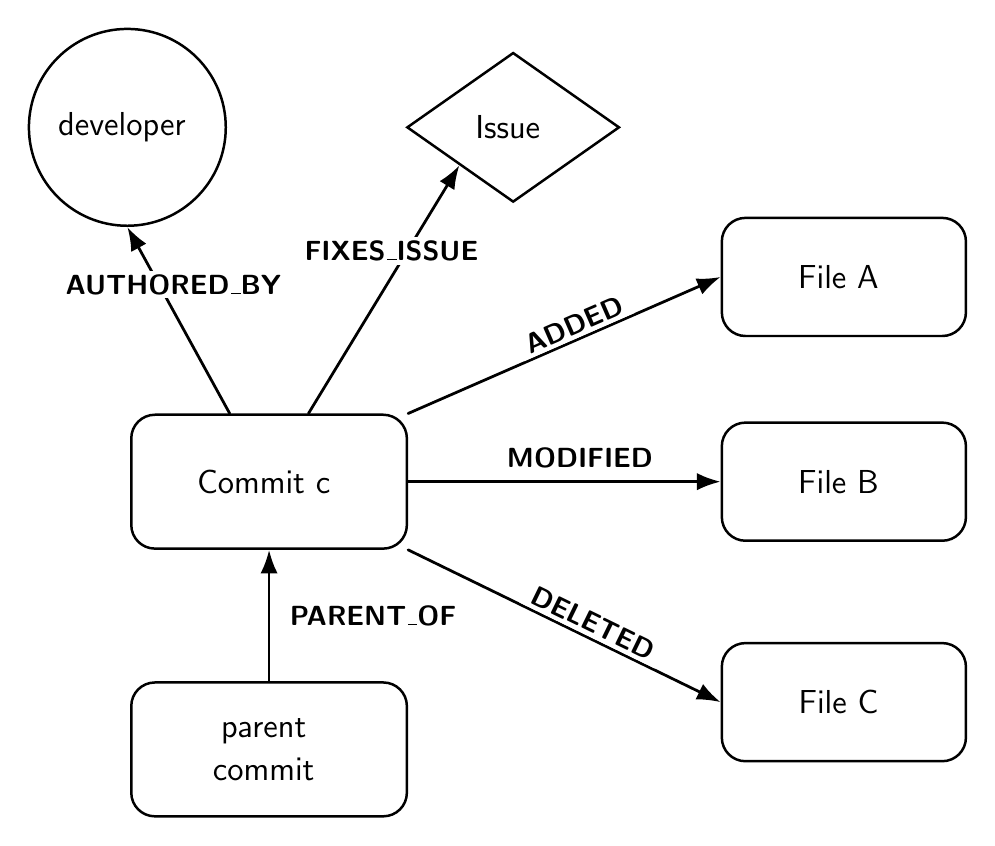
\begin{tikzpicture}

    % ------------------------------------------------------------
    % Nodes
    % ------------------------------------------------------------

    \node[commit node] (commit) at (0,-1.3)
    {
      Commit c
    };

    % Parent commit is now below the main commit
    \node[commit node] (parent) at (0,-4.7)
    {
      \shortstack{
        parent\\[2pt]
        commit
      }
    };

    \node[developer node] (developer) at (-1.8,3.2)
    {
      developer
    };

    \node[issue node] (issue) at (3.1,3.2)
    {
      Issue
    };

    \node[file node] (fileA) at (7.3,1.3)
    {
      File A
    };

    \node[file node] (fileB) at (7.3,-1.3)
    {
      File B
    };

    \node[file node] (fileC) at (7.3,-4.1)
    {
      File C
    };

    % ------------------------------------------------------------
    % Structural relations
    % ------------------------------------------------------------

    % Parent commit to current commit
    \draw[relation]
      (parent.north)
      --
      node[
        relation label,
        right=4pt,
        pos=0.50
      ] {PARENT\_OF}
      (commit.south);

    % Horizontal AUTHORED_BY label
    \draw[relation]
      ([xshift=-5mm]commit.north)
      --
      node[
        relation label,
        above=4pt,
        pos=0.55
      ] {AUTHORED\_BY}
      (developer.south);

    % Horizontal FIXES_ISSUE label
    \draw[relation]
      ([xshift=5mm]commit.north)
      --
      node[
        relation label,
        above=4pt,
        pos=0.55
      ] {FIXES\_ISSUE}
      (issue.south west);

    % ------------------------------------------------------------
    % File-change relations
    % ------------------------------------------------------------

    \draw[relation]
      (commit.north east)
      --
      node[
        relation label,
        sloped,
        above,
        pos=0.55
      ] {ADDED}
      (fileA.west);

    \draw[relation]
      (commit.east)
      --
      node[
        relation label,
        above=3pt,
        pos=0.55
      ] {MODIFIED}
      (fileB.west);

    \draw[relation]
      (commit.south east)
      --
      node[
        relation label,
        sloped,
        above,
        pos=0.57
      ] {DELETED}
      (fileC.west);

    \end{tikzpicture}%
    }

    \caption{Illustration of the Core layer.}
    \label{fig:core-layer}
\end{figure}

\subsubsection{Layer 2: Within-File AST Subgraph}
\label{sec:kg-ast}
The Structural layer represents changes within Java files. Our deployed representation is an AST, built by a deterministic pre-order traversal of the \texttt{javalang} parse tree. For repository-relative path $rel$, the $i$-th visited node receives parse identifier $\{rel\}\code{::A}\{i\}$. Each node stores its \code{javalang} type, a syntactic category, and a compact value such as a name, literal, or operator. Non-blank string children become \code{Identifier} leaves. Ordered containers preserve child order, while unordered containers are canonically sorted. \autoref{fig:deterministic-ast} shows the resulting \edge{HAS_AST} and ordered \edge{AST_CHILD} relations.

\begin{figure}[!htbp]
    \centering

    \resizebox{0.95\columnwidth}{!}{%
    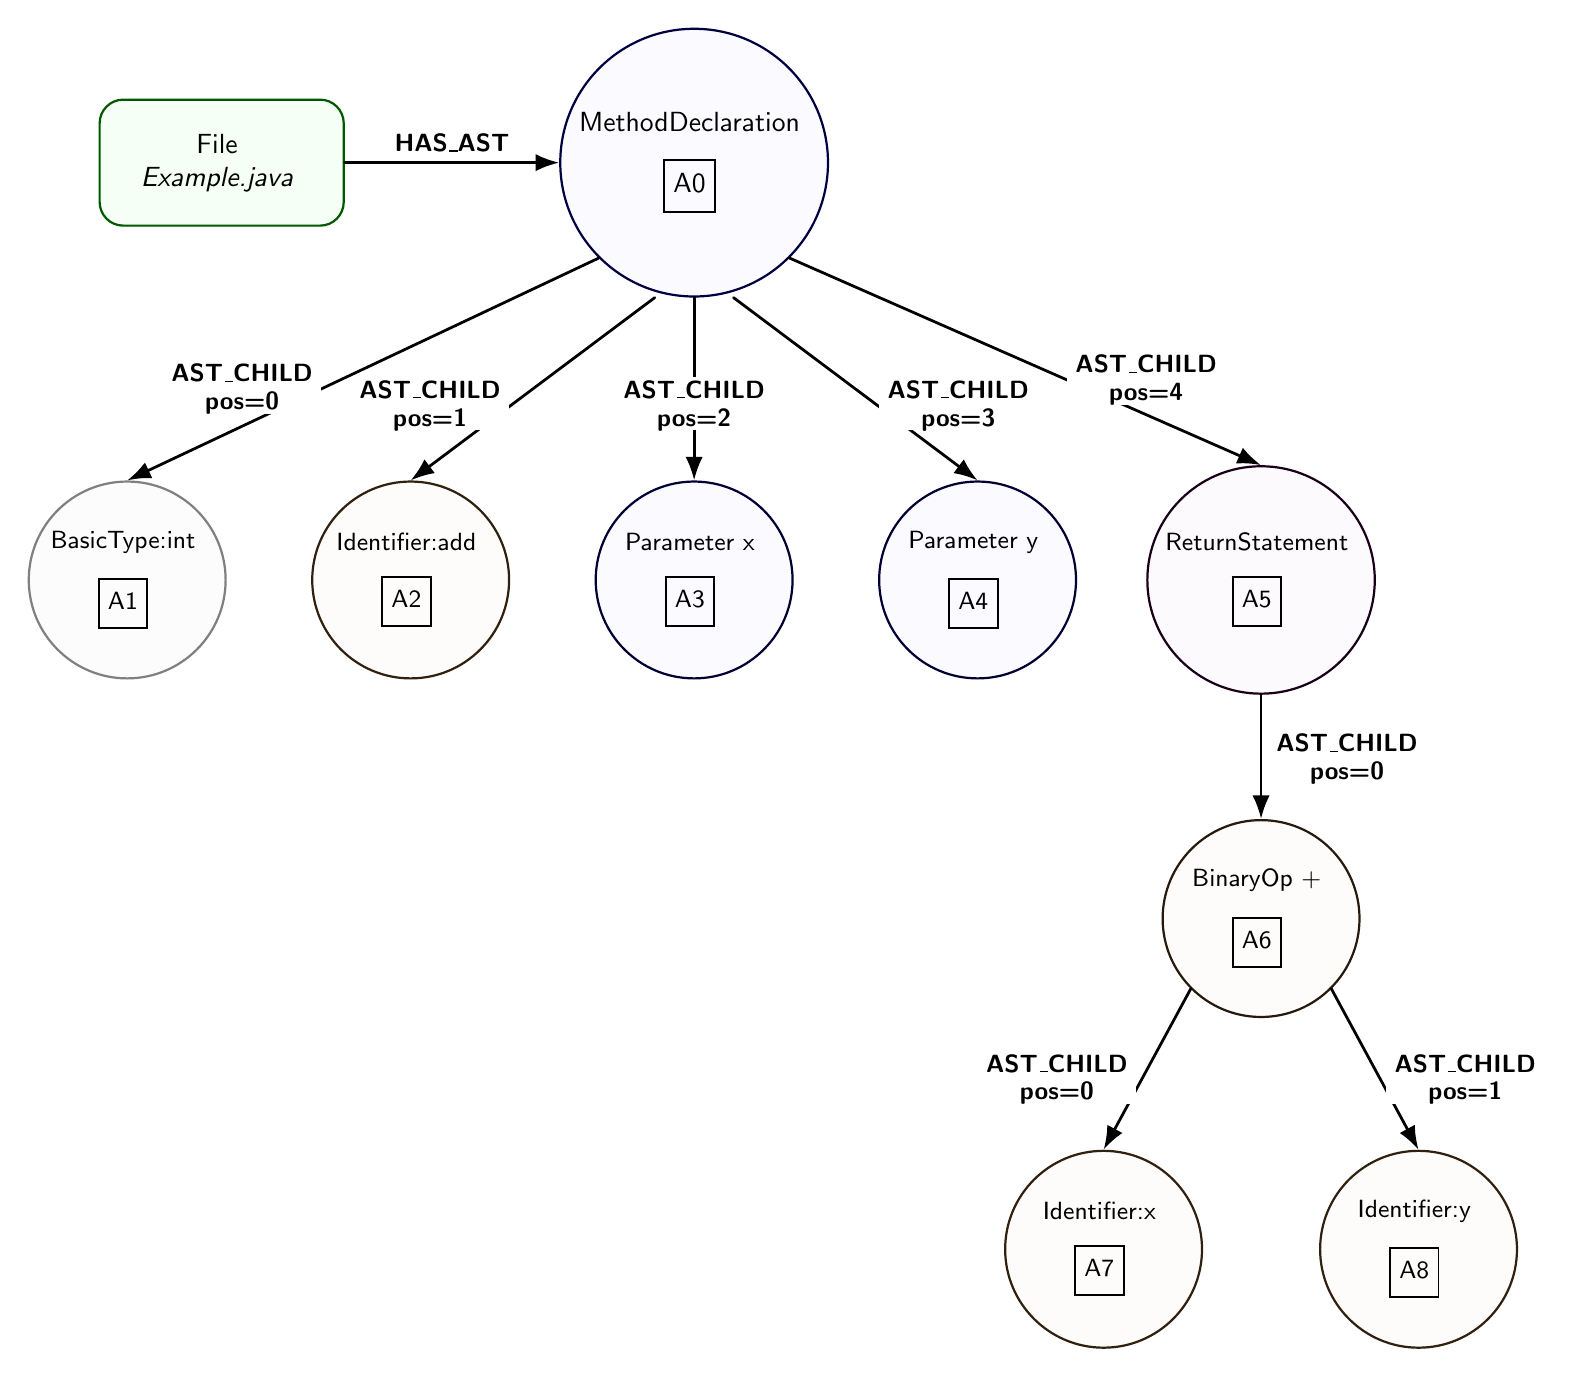
\begin{tikzpicture}

    % ------------------------------------------------------------
    % Nodes
    % ------------------------------------------------------------

    \node[file] (file) at (-6.0,0)
    {
      \shortstack{
        File\\[2pt]
        \textit{Example.java}
      }
    };

    \node[ast root] (A0) at (0,0)
    {
      \shortstack{
        MethodDeclaration\\[7pt]
        \idbox{A0}
      }
    };

    \node[basic type ast] (A1) at (-7.2,-5.3)
    {
      \shortstack{
        BasicType:int\\[6pt]
        \idbox{A1}
      }
    };

    \node[identifier ast] (A2) at (-3.6,-5.3)
    {
      \shortstack{
        Identifier:add\\[6pt]
        \idbox{A2}
      }
    };

    \node[parameter ast] (A3) at (0,-5.3)
    {
      \shortstack{
        Parameter x\\[6pt]
        \idbox{A3}
      }
    };

    \node[parameter ast] (A4) at (3.6,-5.3)
    {
      \shortstack{
        Parameter y\\[6pt]
        \idbox{A4}
      }
    };

    \node[return ast] (A5) at (7.2,-5.3)
    {
      \shortstack{
        ReturnStatement\\[6pt]
        \idbox{A5}
      }
    };

    \node[binaryop ast] (A6) at (7.2,-9.6)
    {
      \shortstack{
        BinaryOp $+$\\[6pt]
        \idbox{A6}
      }
    };

    \node[identifier ast] (A7) at (5.2,-13.8)
    {
      \shortstack{
        Identifier:x\\[6pt]
        \idbox{A7}
      }
    };

    \node[identifier ast] (A8) at (9.2,-13.8)
    {
      \shortstack{
        Identifier:y\\[6pt]
        \idbox{A8}
      }
    };

    % ------------------------------------------------------------
    % Edges
    % ------------------------------------------------------------

    \draw[relation]
      (file.east)
      --
      node[edge label,above=2pt] {HAS\_AST}
      (A0.west);

    \draw[relation]
      (A0.south west)
      --
      node[edge label,pos=0.58,left=1pt]
      {AST\_CHILD\\[-1pt]pos=0}
      (A1.north);

    \draw[relation]
      ([xshift=-5mm]A0.south)
      --
      node[edge label,pos=0.58,left=1pt]
      {AST\_CHILD\\[-1pt]pos=1}
      (A2.north);

    \draw[relation]
      (A0.south)
      --
      node[edge label,pos=0.58]
      {AST\_CHILD\\[-1pt]pos=2}
      (A3.north);

    \draw[relation]
      ([xshift=5mm]A0.south)
      --
      node[edge label,pos=0.58,right=1pt]
      {AST\_CHILD\\[-1pt]pos=3}
      (A4.north);

    \draw[relation]
      (A0.south east)
      --
      node[edge label,pos=0.58,right=1pt]
      {AST\_CHILD\\[-1pt]pos=4}
      (A5.north);

    \draw[relation]
      (A5.south)
      --
      node[edge label,pos=0.50,right=2pt]
      {AST\_CHILD\\[-1pt]pos=0}
      (A6.north);

    \draw[relation]
      (A6.south west)
      --
      node[edge label,pos=0.55,left=2pt]
      {AST\_CHILD\\[-1pt]pos=0}
      (A7.north);

    \draw[relation]
      (A6.south east)
      --
      node[edge label,pos=0.55,right=2pt]
      {AST\_CHILD\\[-1pt]pos=1}
      (A8.north);

    \end{tikzpicture}%
    }
    \caption{Example of the Deterministic construction of the within-file AST subgraph.}
    \label{fig:deterministic-ast}
\end{figure}

\paragraph{AST matching and delta extraction}
For a modified file, let $A^b$ and $A^a$ be the stored and newly parsed ASTs. The matcher constructs a partial injective correspondence $\mu:V(A^b)\rightharpoonup V(A^a)$ in three stages. First, each node is assigned a bottom-up fingerprint: Let
$u_1,\ldots,u_k$ be the ordered children of $v$, and define $h(v)= H\!\left(\ell(v)\Vert h(u_1)\Vert\cdots\Vert h(u_k)\right)$ where $\ell(v)=\code{ast_type}(v)\Vert\code{value}(v)$. Here, $\Vert$ denotes an unambiguous concatenation and $H$ is the MD5
message-digest algorithm \cite{rivest1992md5}. This bottom-up construction is commonly known as subtree hashing or syntax-tree fingerprinting \cite{chilowicz2009syntax}. Equal fingerprints identify candidate identical subtrees. Larger candidate subtrees are processed first, with source position used to break ties, following the general strategy of prioritizing large isomorphic subtrees in AST differencing \cite{falleri2014fine}.

Second, matches are propagated to unmatched parents of the same AST
type until a fixpoint is reached. Third, remaining nodes are matched by $(\code{ast_type},\code{line},\code{column})$ whenever this tuple is unique. The unmatched and changed nodes define the delta:
\begin{align}
  R &= V(A^b)\setminus\operatorname{dom}(\mu),\\
  A &= V(A^a)\setminus\operatorname{ran}(\mu),\\
  U &=
  \left\{
    (b,a)\in\mu \;\middle|\;
    \begin{aligned}
      &\code{ast_type}(b)\neq\code{ast_type}(a)\\
      &{}\lor\ \code{value}(b)\neq\code{value}(a)
    \end{aligned}
  \right\},\\
  M &=
  \left\{
    (b,a)\in\mu \;\middle|\;
    \begin{aligned}
      &\operatorname{par}(b)\in\operatorname{dom}(\mu)\\
      &{}\land\
      \mu(\operatorname{par}(b))
      \neq\operatorname{par}(a)
    \end{aligned}
  \right\}.
\end{align}

Here, $R$, $A$, $U$, and $M$ induce \edge{REMOVES}, \edge{ADDS}, \edge{UPDATES}, and \edge{MOVES}, respectively. In our validation window, the matcher achieved precision and recall of $1.00$, compared with $0.41$ recall for position-only matching (check \autoref{app:??}). \autoref{fig:delta-ast} illustrates the resulting correspondence and edit classes.

\begin{figure}[!htbp]
    \centering
    \resizebox{0.98\columnwidth}{!}{%
    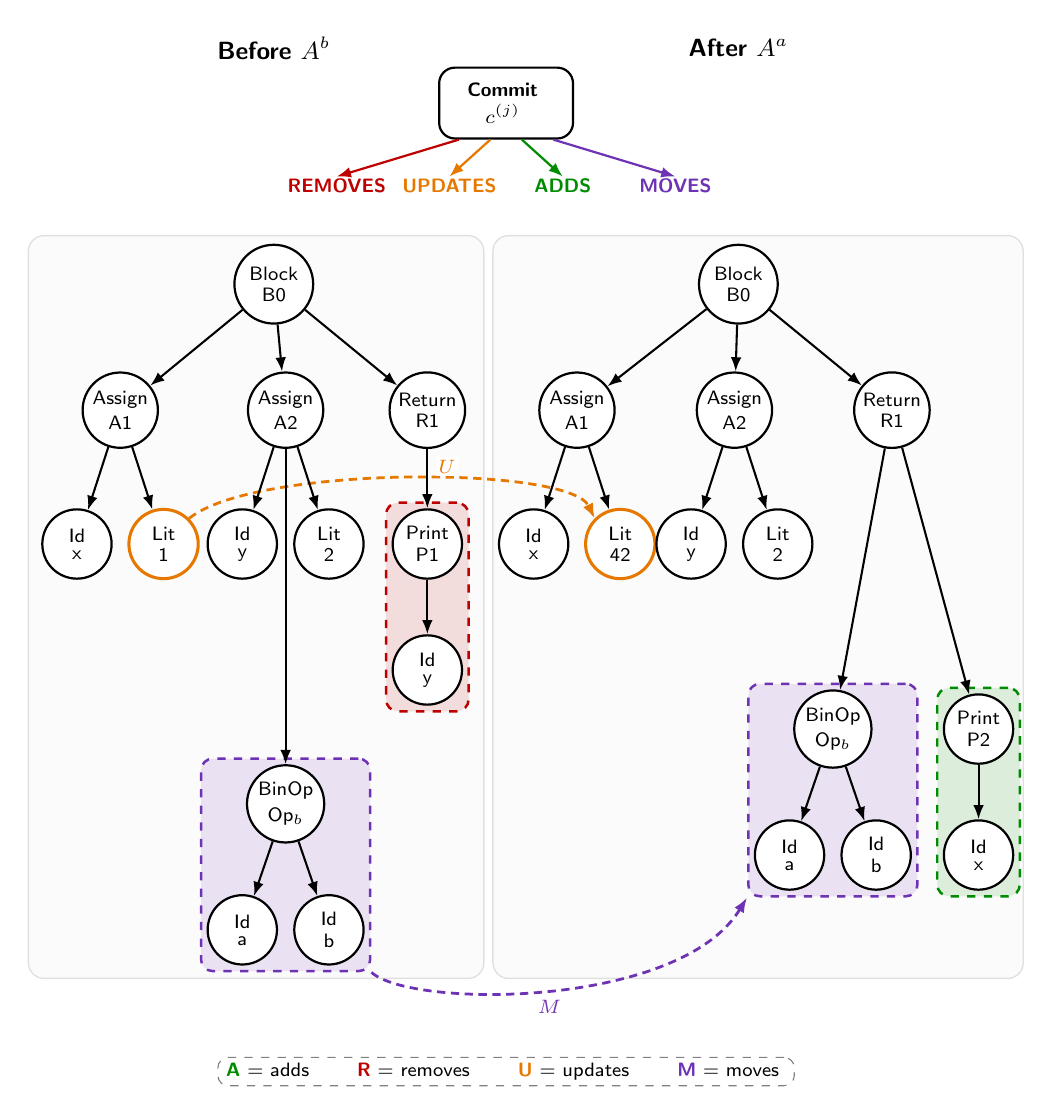
\begin{tikzpicture}[x=1cm,y=1cm]

    % ============================================================
    % Titles
    % ============================================================

    \node[deltaSideTitle] at (-2.95,7.65)
      {Before $A^b$};

    \node[deltaSideTitle] at (2.95,7.65)
      {After $A^a$};

    % ============================================================
    % Commit and four possible delta operations
    % ============================================================

    \node[deltaCommit] (commit) at (0,6.95)
    {
      \shortstack{
        \textbf{Commit}\\
        $c^{(j)}$
      }
    };

    \node[
      deltaTopLabel,
      text=deltaRemC
    ] (remLbl) at (-2.15,5.90)
      {REMOVES};

    \node[
      deltaTopLabel,
      text=deltaUpdC
    ] (updLbl) at (-0.72,5.90)
      {UPDATES};

    \node[
      deltaTopLabel,
      text=deltaAddC
    ] (addLbl) at (0.72,5.90)
      {ADDS};

    \node[
      deltaTopLabel,
      text=deltaMovC
    ] (movLbl) at (2.15,5.90)
      {MOVES};

    \draw[
      -{Latex[length=1.8mm,width=1.35mm]},
      draw=deltaRemC,
      line width=0.8pt
    ]
      ([xshift=-6mm]commit.south)
      --
      (remLbl.north);

    \draw[
      -{Latex[length=1.8mm,width=1.35mm]},
      draw=deltaUpdC,
      line width=0.8pt
    ]
      ([xshift=-2mm]commit.south)
      --
      (updLbl.north);

    \draw[
      -{Latex[length=1.8mm,width=1.35mm]},
      draw=deltaAddC,
      line width=0.8pt
    ]
      ([xshift=2mm]commit.south)
      --
      (addLbl.north);

    \draw[
      -{Latex[length=1.8mm,width=1.35mm]},
      draw=deltaMovC,
      line width=0.8pt
    ]
      ([xshift=6mm]commit.south)
      --
      (movLbl.north);

    % ============================================================
    % Before tree
    % ============================================================

    \node[deltaRoot] (Bb0) at (-2.95,4.65)
      {\shortstack{Block\\B0}};

    \node[deltaAst] (BA1) at (-4.90,3.05)
      {\shortstack{Assign\\A1}};

    \node[deltaAst] (BA2) at (-2.80,3.05)
      {\shortstack{Assign\\A2}};

    \node[deltaAst] (BR1) at (-1.00,3.05)
      {\shortstack{Return\\R1}};

    \draw[deltaEdge] (Bb0) -- (BA1);
    \draw[deltaEdge] (Bb0) -- (BA2);
    \draw[deltaEdge] (Bb0) -- (BR1);

    % Assign A1 children
    \node[deltaAst] (BIdx) at (-5.45,1.35)
      {\shortstack{Id\\x}};

    \node[deltaUpdated] (BLit1) at (-4.35,1.35)
      {\shortstack{Lit\\1}};

    \draw[deltaEdge] (BA1) -- (BIdx);
    \draw[deltaEdge] (BA1) -- (BLit1);

    % Assign A2 children
    \node[deltaAst] (BIdy) at (-3.35,1.35)
      {\shortstack{Id\\y}};

    \node[deltaAst] (BLit2) at (-2.25,1.35)
      {\shortstack{Lit\\2}};

    \draw[deltaEdge] (BA2) -- (BIdy);
    \draw[deltaEdge] (BA2) -- (BLit2);

    % Removed subtree
    \node[deltaAst] (BP1) at (-1.00,1.35)
      {\shortstack{Print\\P1}};

    \node[deltaAst] (BRemId) at (-1.00,-0.25)
      {\shortstack{Id\\y}};

    \draw[deltaEdge] (BR1) -- (BP1);
    \draw[deltaEdge] (BP1) -- (BRemId);

    % Moved subtree in the before tree
    \node[deltaAst] (BOp) at (-2.80,-1.95)
      {\shortstack{BinOp\\Op$_b$}};

    \node[deltaAst] (BOpA) at (-3.35,-3.55)
      {\shortstack{Id\\a}};

    \node[deltaAst] (BOpB) at (-2.25,-3.55)
      {\shortstack{Id\\b}};

    \draw[deltaEdge]
      (BA2.south)
      --
      (BOp.north);

    \draw[deltaEdge] (BOp) -- (BOpA);
    \draw[deltaEdge] (BOp) -- (BOpB);

    % ============================================================
    % After tree
    % ============================================================

    \node[deltaRoot] (Ab0) at (2.95,4.65)
      {\shortstack{Block\\B0}};

    \node[deltaAst] (AA1) at (0.90,3.05)
      {\shortstack{Assign\\A1}};

    \node[deltaAst] (AA2) at (2.90,3.05)
      {\shortstack{Assign\\A2}};

    \node[deltaAst] (AR1) at (4.90,3.05)
      {\shortstack{Return\\R1}};

    \draw[deltaEdge] (Ab0) -- (AA1);
    \draw[deltaEdge] (Ab0) -- (AA2);
    \draw[deltaEdge] (Ab0) -- (AR1);

    % Assign A1 children
    \node[deltaAst] (AIdx) at (0.35,1.35)
      {\shortstack{Id\\x}};

    \node[deltaUpdated] (ALit42) at (1.45,1.35)
      {\shortstack{Lit\\42}};

    \draw[deltaEdge] (AA1) -- (AIdx);
    \draw[deltaEdge] (AA1) -- (ALit42);

    % Assign A2 children
    \node[deltaAst] (AIdy) at (2.35,1.35)
      {\shortstack{Id\\y}};

    \node[deltaAst] (ALit2) at (3.45,1.35)
      {\shortstack{Lit\\2}};

    \draw[deltaEdge] (AA2) -- (AIdy);
    \draw[deltaEdge] (AA2) -- (ALit2);

    % Moved subtree in the after tree
    \node[deltaAst] (AOp) at (4.15,-1.00)
      {\shortstack{BinOp\\Op$_b$}};

    \node[deltaAst] (AOpA) at (3.60,-2.60)
      {\shortstack{Id\\a}};

    \node[deltaAst] (AOpB) at (4.70,-2.60)
      {\shortstack{Id\\b}};

    \draw[deltaEdge] (AR1) -- (AOp);
    \draw[deltaEdge] (AOp) -- (AOpA);
    \draw[deltaEdge] (AOp) -- (AOpB);

    % Added subtree
    \node[deltaAst] (AP2) at (6.00,-1.00)
      {\shortstack{Print\\P2}};

    \node[deltaAst] (AAddId) at (6.00,-2.60)
      {\shortstack{Id\\x}};

    \draw[deltaEdge] (AR1) -- (AP2);
    \draw[deltaEdge] (AP2) -- (AAddId);

    % ============================================================
    % Background highlight regions and update correspondence
    % ============================================================

    \begin{pgfonlayer}{background}

      % ------------------------------------------------------------
    % Symmetric gray panels behind each tree
    % Same height, with a small gap between them
    % ------------------------------------------------------------
    
    \coordinate (BeforePanelNW) at (-5.95,5.15);
    \coordinate (BeforePanelSE) at (-0.40,-4.05);
    
    \coordinate (AfterPanelNW)  at ( -0.05,5.15);
    \coordinate (AfterPanelSE)  at ( 6.45,-4.05);
    
    \node[
      deltaTreePanel,
      fit=(BeforePanelNW)(BeforePanelSE)
    ] (BeforePanel) {};
    
    \node[
      deltaTreePanel,
      fit=(AfterPanelNW)(AfterPanelSE)
    ] (AfterPanel) {};
    
      % Delta highlight boxes
      \node[
        deltaRemoveBox,
        fit=(BP1)(BRemId)
      ] (Rbox) {};

      \node[
        deltaMoveBox,
        fit=(BOp)(BOpA)(BOpB)
      ] (BMoveBox) {};

      \node[
        deltaMoveBox,
        fit=(AOp)(AOpA)(AOpB)
      ] (AMoveBox) {};

      \node[
        deltaAddBox,
        fit=(AP2)(AAddId)
      ] (Ibox) {};

      % Updated-node correspondence
      \draw[
        -{Latex[length=1.9mm,width=1.4mm]},
        draw=deltaUpdC,
        line width=1pt,
        densely dashed
      ]
        (BLit1.north east)
        ..
        controls (-3.20,2.35) and (0.80,2.35)
        ..
        (ALit42.north west);

    \end{pgfonlayer}

    \node[
      deltaRelationLabel,
      text=deltaUpdC
    ] at (-0.75,2.33)
      {$U$};

    % ============================================================
    % Moved-subtree correspondence
    % ============================================================

    \draw[
      -{Latex[length=1.9mm,width=1.4mm]},
      draw=deltaMovC,
      line width=1pt,
      densely dashed
    ]
      (BMoveBox.south east)
      ..
      controls (-1.20,-4.55) and (2.20,-4.55)
      ..
      (AMoveBox.south west);

    \node[
      deltaRelationLabel,
      text=deltaMovC
    ] at (0.55,-4.53)
      {$M$};

    % ============================================================
    % Legend
    % ============================================================

    \node[deltaLegend] at (0,-5.35)
    {
      \textcolor{deltaAddC}{\textbf{A}} = adds
      \qquad
      \textcolor{deltaRemC}{\textbf{R}} = removes
      \qquad
      \textcolor{deltaUpdC}{\textbf{U}} = updates
      \qquad
      \textcolor{deltaMovC}{\textbf{M}} = moves
    };

    \end{tikzpicture}%
    }
    \caption{Simplified illustration of AST deltas between the before tree $A^b$ and the after tree $A^a$.}
    \label{fig:delta-ast}
\end{figure}

\paragraph{Online delta maintenance.}
Commits are processed in chronological order while the system retains, for each tracked file, its current AST and the mapping from parse identifiers to persistent graph identifiers. Added files are materialized once, files first encountered as modifications are initialized from their parent revision, and deleted files have their live nodes marked inactive. During a modification, matched nodes retain their identifiers, inserted nodes receive new identifiers, and removed nodes remain queryable through \code{alive}$=\textsc{false}$. The live \edge{AST_CHILD} relations are updated in place, while the commit stores only the resulting \edge{ADDS}, \edge{REMOVES}, \edge{UPDATES}, and \edge{MOVES} relations. Thus, storage and update costs follow the amount of syntactic change.

\paragraph{Alternative within-file representations.}
Besides AST, we evaluate control-flow (CFG), data-flow (DFG), and program-dependency graph (PDG). All representations use the same matching and delta extraction methods used for AST. \autoref{app:alternative-subgraphs} provides an example of these alternative subgraphs.

\subsubsection{Layer 3: Commit Semantic-Text Graph (CSTG)}
\label{sec:kg-cstg}
The third layer represents the semantics of a change using its commit message and diff text. For each commit $c$, we concatenate the message with lexical tokens from changed lines to form $x_c$. The text is tokenized and lower-cased, camel-case identifiers are split, and defect-relevant identifiers such as \texttt{*Exception} and \texttt{*Error} are preserved. Terms are assigned types in $\{\text{code},\text{bug},\text{action},\text{error},\text{natural-language}\}$. Each commit yields a graph-of-words whose terms are linked to the commit through weighted \edge{MENTIONS} relations. Across the training corpus, associated terms are connected through \edge{COOCCURS}, and each term receives a propagated defect-risk score. Commits are also linked to \node{Intent} nodes through \edge{HAS_INTENT}; when a term is equal to an element represented in the second layer (\autoref{sec:kg-ast}), an optional \edge{GROUNDS_IN} relation connects it to the corresponding AST leaf. The resulting CSTG schema is illustrated in \autoref{fig:cstg-schema}.

\begin{figure}[!htbp]
    \centering
    \includegraphics[width=\columnwidth]
        {methodology/cstg_layer.png}
    \caption{CSTG schema for a commit. Darker term nodes indicate higher propagated defect risk.}
    \label{fig:cstg-schema}
\end{figure}

\paragraph{Graph-of-words, term weighting, and propagated risk}
For each commit $c$, let $V_c$ be the distinct normalized terms in $x_c$. We construct a weighted graph-of-words $G_c^{\mathrm{text}}=(V_c,E_c,\omega_c)$ by connecting terms occurring within a window of $w$ tokens (\cite{rousseau2013graph}), where $\omega_c(u,v)$ is their number of within-window co-occurrences. This representation retains local term dependencies that are discarded by a bag-of-words model \cite{rousseau2015main}. We compute a weighted TextRank score $\mathrm{TR}_c(t)$ for each term using damping factor $d$ \cite{mihalcea2004textrank}, and weight the corresponding \edge{MENTIONS} relation by
\begin{align}
m_c(t)
=
\mathrm{TR}_c(t)
\log\!\left(
\frac{|C_{\mathrm{tr}}|+1}{\mathrm{df}(t)+1}
\right),
\end{align}
where $C_{\mathrm{tr}}$ is the training corpus and $\mathrm{df}(t)$ is the number of training commits containing $t$. Thus, $m_c(t)$ combines within-commit term centrality with corpus-level rarity; it can be viewed as a TextRank-based variant of graph term-weight IDF
\cite{rousseau2013graph}.

To construct the global term graph, let $p(t)$ be the fraction of
training commits containing $t$, and let $p(t_i,t_j)$ be the fraction
containing both terms. Their association is measured using normalised pointwise mutual information (NPMI), an extension of pointwise mutual information for association measurement \cite{church1990word,bouma2009normalized}.:
\begin{align}
\operatorname{NPMI}(t_i,t_j)
=
\frac{
\log\!\left(p(t_i,t_j)/(p(t_i)p(t_j))\right)
}{
-\log p(t_i,t_j)
}.
\end{align}
Let $n_{ij}$ be the number of training commits containing both terms.
The \edge{COOCCURS} adjacency matrix is defined as
\begin{align}
(A_{\mathrm T})_{ij}
=
\begin{cases}
\operatorname{NPMI}(t_i,t_j),
&
n_{ij}\geq n_{\min}
\ \land\
\operatorname{NPMI}(t_i,t_j)\geq\tau_{\mathrm T},
\\
0, & \text{otherwise},
\end{cases}
\end{align}
where $n_{\min}$ removes poorly supported associations and
$\tau_{\mathrm T}>0$ retains only sufficiently strong positive
associations. Finally, let $\mathrm{bugdf}(t)$ be the number of bug-inducing training commits containing $t$, and let $\bar y$ be the training bug rate. We initialise the defect risk of $t$ using the smoothed estimate
\begin{align}
r^{(0)}(t)
=
\frac{\mathrm{bugdf}(t)+\lambda\bar y}
     {\mathrm{df}(t)+\lambda},
\qquad \lambda>0.
\end{align}
Let $P_{\mathrm T}$ be the row-normalised form of $A_{\mathrm T}$,
with $(P_{\mathrm T})_{tt}=1$ for an otherwise isolated term. Risk is
propagated according to $
r^\star
=
(1-\alpha_{\mathrm T})r^{(0)}
+
\alpha_{\mathrm T}P_{\mathrm T}r^\star,
$, $\alpha_{\mathrm T}\in(0,1)$, which imposes a smoothness prior over associated terms while retaining the observed term-specific risk \cite{belkin2006manifold}. The resulting $r^\star(t)$ is stored on the corresponding \node{Term} node. An example of the resulting global term graph is shown in
\autoref{fig:cstg-term-graph}.

\begin{figure}[!htbp]
    \centering
    \includegraphics[width=0.98\columnwidth]
        {methodology/cstg_term_graph.png}
    \caption{Example global CSTG term graph. Edges denote retained positive NPMI associations, and node colour indicates propagated term risk $r^{\star}(t)$.}
    \label{fig:cstg-term-graph}
\end{figure}

% \paragraph{Leakage-free online use.}
% The vocabulary, document frequencies, NPMI graph, and propagated risks are estimated from $C_{\mathrm{tr}}$ and then frozen. An incoming commit contributes only its own \edge{MENTIONS}, \edge{HAS_INTENT}, and optional \edge{GROUNDS_IN} relations.

\subsubsection{Inference over KG-Commit}
\label{sec:kg-infer}

We use five graph-based inference channels: Relational Neighbour
(RN)~\cite{macskassy2003probabilistic}, Personalised PageRank
(PPR)~\cite{haveliwala2002topic}, clamped Label
Propagation (LP)~\cite{zhu2003semi}, DeepWalk matrix factorisation
(DW)~\cite{perozzi2014deepwalk,qiu2018network}, and DistMult
knowledge-graph embedding (KGE)~\cite{yang2015embedding}. A sixth, feature-based CSTG channel uses the semantic statistics introduced in \autoref{sec:kg-cstg}. Their outputs are combined by logistic stacking~\cite{wolpert1992stacked} to create a fusion score. Labels are restricted to the gap-resolved commits defined in \autoref{sec:operational-constraints}; this set is denoted by $\mathcal{C}_{\mathrm{past}}$. Full procedures are given in Algorithms~\ref{alg:hub}--\ref{alg:gchannel} of \autoref{app:supporting-algorithms}.

\paragraph{Shared commit-hub projection}
A \emph{hub} is an inference-level abstraction for a context item shared by commits: a developer, file, structural change-token, or CSTG \node{Term}. For an observable commit $c$ and hub $h$, let $\operatorname{tf}(c,h)$ be the number of observed occurrences of $h$ in $c$. The weighted commit-hub incidence matrix is
\begin{equation}
C_{ch}
=
\operatorname{tf}(c,h)
\left[
1+
\log\left(
\frac{
|\mathcal{C}_{\mathrm{past}}|+1
}{
\operatorname{df}_{\mathrm{past}}(h)+1
}
\right)
\right].
\end{equation}
where $\operatorname{df}_{\mathrm{past}}(h)$ is the number of connected commits connected to $h$. With
\begin{equation}
A_{\mathrm{G}}
=
\begin{bmatrix}
0 & C\\
C^{\top} & 0
\end{bmatrix},
\qquad
P
=
A_{\mathrm{G}}
\operatorname{diag}
\left(A_{\mathrm{G}}^{\top}\mathbf{1}\right)^{\dagger}.
\end{equation}

\paragraph{CSTG semantic channel}
The CSTG channel assigns defect risk to \node{Term} nodes described in \autoref{sec:kg-cstg}. Its main risk feature is
\begin{equation}
\rho(c)
=
\frac{
\sum_{t\in V_c}\mathrm{TR}_c(t)r^{\star}(t)
}{
\sum_{t\in V_c}\mathrm{TR}_c(t)+\varepsilon
}.
\end{equation}

\paragraph{Score fusion}
The six channel probabilities are combined by
\begin{equation}
\widehat{y}(c)
=
\sigma\left(
\theta_0+
\sum_{m\in\mathcal{M}}\theta_m s_m(c)
\right),
\end{equation}
where $\mathcal{M}=\{\mathrm{RN},\mathrm{PPR},\mathrm{LP},\mathrm{DW},\mathrm{KGE}\}$.

% \subsubsection{Online Protocol and Model Selection}
% \label{sec:kg-protocol}
% Commits are processed chronologically under the warm-up and gap constraints of \autoref{sec:operational-constraints}. For each target commit block, its observable entities and relations are first added to the graph as described in \autoref{sec:kg_evolution}; the commit is then scored using only the labels currently available. Trainable models and the decision threshold are periodically updated from past data only, with the threshold selected to maximize Buggy-F1. 
% To choose the graph-based fusion, we evaluate every non-empty subset $S$ of the five graph channels, retain those satisfying $\mathrm{MF1}(S)\geq\mathrm{MF1}^{\star}-\tau$, and select $F=\arg\min_S\bigl(|S|,-\mathrm{MF1}(S)\bigr)$. Thus, Macro-F1 is the primary criterion, with the number of channels used to prefer a simpler near-optimal model. The CSTG channel $G$ is added only when it improves the past-only validation score. The warm-up, gap, block size, and tolerance $\tau$ are specified in \autoref{sec:??}.

\section{Experimental Design}
\subsection{Research Questions}

\begin{itemize}
    \item \textbf{RQ1.} \emph{What is the predictive performance of the proposed KG-Commit representation in Just-in-Time Software Defect Prediction?}
    \vspace{1em}
    \item \textbf{RQ2.} \emph{How well does KG-Commit maintain computational efficiency and scalability across the real-time evolution of different software projects?}
    \vspace{1em}
    \item \textbf{RQ3.} \emph{How do architectural choices regarding fine-grained code subgraph representations and distinct KG layers affect the predictive performance of KG-Commit?}
    \vspace{1em}
    \item \textbf{RQ4.} \emph{How does predictive performance vary across inference methods when applied to the KG-Commit representation?}
\end{itemize}

\subsection{Dataset}
\label{sec:dataset}

We evaluate our approach on ApacheJIT~\cite{keshavarz2022apachejit}, one of the largest public datasets for just-in-time defect prediction. It contains 106{,}674 commits from 14 popular Apache projects written in Java, of which 28{,}239 are bug-inducing and 78{,}435 are clean, giving a bug-inducing ratio of about 26\% (Table~\ref{tab:projects}). Labels are produced by the SZZ algorithm~\cite{sliwerski2005changes} and their quality is improved by linking fixes to issue reports, keeping only Java changes, and removing trivial edits with GumTree over abstract syntax trees, following the filtering steps of prior work~\cite{mcintosh2018fix}.

Each commit is described by fourteen fields: a commit identifier, the binary
bug-inducing label, and twelve change metrics that follow the definitions of
Kamei et al.~\cite{kamei2013large}, grouped into the four dimensions shown in
Table~\ref{tab:features}. Because these metrics are highly right-skewed we apply
a logarithmic transform, and because just-in-time prediction is an online task we
split each project in time order and train only on commits that precede the test
commits~\cite{kamei2013large,cabral2023towards}. The class imbalance is handled at
training time through cost-sensitive learning.

\begin{table}[t]
\centering
\caption{Projects in the ApacheJIT dataset~\cite{keshavarz2022apachejit}.
Percentages give the ratio of bug-inducing commits to total commits.}
\label{tab:projects}
\small
\begin{tabular}{lrrr}
\toprule
Project & Bug-inducing & Clean & Total \\
\midrule
ActiveMQ  & 1{,}404 (23\%) & 4{,}722  & 6{,}126 \\
Camel     & 3{,}078 (14\%) & 19{,}622 & 22{,}700 \\
Cassandra & 3{,}117 (38\%) & 5{,}042  & 8{,}159 \\
Flink     & 2{,}811 (24\%) & 8{,}880  & 11{,}691 \\
Groovy    & 1{,}614 (20\%) & 6{,}445  & 8{,}059 \\
HDFS      & 2{,}222 (21\%) & 8{,}137  & 10{,}359 \\
HBase     & 3{,}782 (43\%) & 4{,}948  & 8{,}730 \\
Hive      & 4{,}223 (61\%) & 2{,}619  & 6{,}842 \\
Ignite    & 2{,}439 (20\%) & 9{,}597  & 12{,}036 \\
MapReduce & 838 (15\%)     & 4{,}995  & 5{,}833 \\
Kafka     & 1{,}115 (46\%) & 1{,}269  & 2{,}384 \\
Spark     & 632 (43\%)     & 833      & 1{,}465 \\
Zeppelin  & 622 (42\%)     & 829      & 1{,}451 \\
Zookeeper & 342 (40\%)     & 497      & 839 \\
\midrule
\textbf{Total} & \textbf{28{,}239 (26\%)} & \textbf{78{,}435} & \textbf{106{,}674} \\
\bottomrule
\end{tabular}
\end{table}

% Required in your preamble: \usepackage{tabularx} \usepackage{booktabs}

\begin{table}[t]
\centering
\caption{The fourteen fields of ApacheJIT. The twelve change metrics follow Kamei et al.~\cite{kamei2013large}.}
\label{tab:features}
\footnotesize % Slightly smaller font size to optimize single-column space
\setlength{\tabcolsep}{4pt} % Tightens horizontal padding between columns
\begin{tabularx}{\columnwidth}{llX}
\toprule
Field & Dimension & Description \\
\midrule
\texttt{commit\_id} & Identifier & Hash of the commit. \\
\texttt{la}         & Size       & Number of lines added. \\
\texttt{ld}         & Size       & Number of lines deleted. \\
\texttt{nf}         & Diffusion  & Number of modified files. \\
\texttt{nd}         & Diffusion  & Number of modified directories. \\
\texttt{ns}         & Diffusion  & Number of modified subsystems. \\
\texttt{ent}        & Diffusion  & Entropy of the change across the modified files. \\
\texttt{ndev}       & History    & Number of developers who previously changed the files. \\
\texttt{age}        & History    & Average time since the last change to the files. \\
\texttt{nuc}        & History    & Number of unique prior changes to the files. \\
\texttt{aexp}       & Experience & Overall experience of the author. \\
\texttt{arexp}      & Experience & Recent experience of the author. \\
\texttt{asexp}      & Experience & Experience of the author on the subsystem. \\
\texttt{buggy}      & Target     & $1$ if the commit is bug-inducing, else $0$. \\
\bottomrule
\end{tabularx}
\end{table}


\subsection{Baselines}
\label{sec:setup-baselines-section}

We compare KG-Commit against ten reference predictors. All run on the same online engine of Section~\ref{sec:setup-protocol-section}, so any gap traces to the input representation and the classifier rather than to evaluation choices.

Three baselines operate on the twelve ApacheJIT change metrics~\cite{keshavarz2022apachejit} and use neither the graph nor commit text. \textbf{LR} is a class-weighted logistic regression. It is the canonical linear just-in-time model and the like-for-like control for KG-Commit's fusion head. \textbf{RF} is a class-weighted random forest of 200 trees and captures interactions the linear model cannot. \textbf{GBoost} is a \texttt{HistGradientBoosting} classifier and sets the strongest change-metric bar.

Three further baselines reproduce published methods under our protocol instead of copying their reported numbers, because those studies use random or single time splits that online results cannot be compared against. \textbf{LApredict}~\cite{zeng2021deep} regresses on the added-line count alone. \textbf{Deeper}~\cite{yang2015deep} feeds a nonlinear autoencoder code of the metrics, concatenated with the raw metrics, into a logistic regression; it stands in for the original DBN, whose maintained libraries are unavailable. \textbf{JITLine}~\cite{pornprasit2021jitline} trains a random forest on the expert metrics joined with per-commit diff-token counts, with the vocabulary fit on the warm-up window. We reproduce its commit-level prediction and omit the line-level LIME step.

We add no separate row for Yan et al.'s prediction-and-localization framework. Its prediction stage is a logistic regression over expert change metrics and is already covered by \textbf{LR}, and its $N$-gram localization is a line-level task outside our scope.

Three non-learned references calibrate the metrics against each project's class balance. \textbf{All-buggy} labels every commit defective, \textbf{All-benign} labels none, and \textbf{Base-rate} scores each commit by the bug rate of all strictly earlier commits. A high raw F1 that All-buggy also attains flags a metric driven by imbalance rather than by discrimination.

\subsection{Experimental Protocol}
\label{sec:setup-protocol-section}

Evaluation follows a prequential, strictly chronological protocol. Commits are processed in author-timestamp order; the model predicts each label from the graph state and statistics of earlier commits, after which the true label is revealed and the graph updated. The first 40\% of each project's stream serves as an unscored warm-up and the remaining 60\% is evaluated. Although predictions are made per commit, models are refit at block granularity on the expanding historical window, which tracks concept drift at tractable cost. Every learned component (scalers, vectorisers, weighting schemes, risk priors, embedding bases, stacking regressions) is fit on past data only. Propagation and random-walk seeds exclude the commit under test, and text features use a stateless hashed representation, so no future information leaks into any prediction.

Comparisons vary one factor at a time: representations under a fixed inference method, and inference methods under a fixed representation. The warm-up proportion, refit schedule, and classifier family stay constant throughout. For deployment, we select the smallest combination of inference methods whose aggregate performance lies within a fixed tolerance of the best combination, adding further channels only when they measurably improve performance.

Within-project baselines run under the same online protocol. We also compare against a previously published external baseline by reproducing that work's single chronological split with a matched classifier, so any difference reflects the input representation rather than the learning algorithm. These single-split results are reported separately, and the within-project baseline is checked against values previously reported on that split. Statistical reliability rests on paired, per-commit out-of-sample scores, assessed with DeLong's test under Holm correction, paired bootstrap confidence intervals, and Cliff's $\delta$.

\subsection{Experimental Settings}
\label{sec:setup-settings-section}

All experiments, including graph construction, ran on a single laptop with no GPU or cluster: Windows~11 (64-bit), an Intel Core i7-13620H (10~cores/16~threads, 2.4\,GHz), and 16\,GB RAM. The pipeline is pure Python plus a Dockerised Neo4j server and does not depend on the operating system. On disk, the graph store occupies about 3.3\,GB (5.6\,GB with transaction logs). \autoref{tab:setup-versions} lists the software stack; no deep-learning framework is used at any stage.
\begin{table}[t]
\centering
\caption{Software and library versions.}
\label{tab:setup-versions}
\footnotesize
\setlength{\tabcolsep}{3pt}
\begin{tabularx}{\columnwidth}{llX}
\toprule
Component & Version & Role \\
\midrule
Python & 3.13.5 & pipeline runtime \\
Neo4j (Community) & 2026.05 & graph store (Dockerised) \\
\texttt{neo4j} driver & 6.2.0 & Bolt driver \\
git & 2.45.1 & commit blob/diff retrieval \\
javalang & 0.13.0 & Java parsing \\
NumPy & 2.2.6 & array/graph kernels \\
SciPy & 1.16.2 & sparse matrices, statistical tests \\
scikit-learn & 1.7.2 & logistic-regression heads, baselines \\
pandas & 2.3.2 & tabular handling \\
networkx & 3.5 & in-memory graph construction \\
matplotlib & 3.10.6 & figures \\
PyYAML & 6.0.2 & configuration \\
\bottomrule
\end{tabularx}
\end{table}

\autoref{lst:core} gives the Core-layer build query in the form used in all runs. Statement~(1) upserts an entity by primary key. Because \texttt{MERGE} matches before it creates, re-ingesting a commit rewrites its properties instead of duplicating the node, which is what makes an interrupted build resumable. Statement~(2) writes the process edges of one commit in a single round trip: \texttt{UNWIND} expands a parameter list of targets into rows, and each row merges its target node and the edge to it. Node labels, edge types, and property maps are supplied as parameters, so one query serves every rule in the Core layer. The AST and CSTG layers use the same two shapes with different labels; the full set is in \autoref{app:cypher-queries}.

\begin{lstlisting}[
style=cypher,
caption={Core layer: idempotent node upsert and batched relationship creation (representative instantiation; \texttt{Commit}/\texttt{File}/\texttt{MODIFIED} are templated per rule).},
label={lst:core}
]
// (1) upsert an entity node by primary key
MERGE (e:Commit {id: $pk_value})
  ON CREATE SET e += $props
  ON MATCH  SET e += $props
// (2) batch-create the process edges from one source node
MATCH (src:Commit {id: $src_id})
UNWIND $targets AS t
  MERGE (tgt:File {id: t.target_id})
  MERGE (src)-[r:MODIFIED]->(tgt)
    ON CREATE SET r += t.props
\end{lstlisting}

% Added hyperparameters table from Appendix of Sina
\begin{table}[!htbp]\centering\small\setlength{\tabcolsep}{5pt}
\caption{Appendix B: complete hyperparameters, protocol constants, and environment
for KG-Commit. All learned components use class-weighted losses; all statistics are
fit on strictly-past data.}
\label{tab:hyperparams}
\resizebox{\linewidth}{!}{%
\begin{tabular}{lll}
\toprule
Group & Parameter & Value \\
\midrule
\multirow{4}{*}{Online protocol}
 & Warm-up fraction $K$        & $0.40$ (Setting A); $0.20$ (Setting B) \\
 & Block size $M$              & $200$ \\
 & Verification-latency gap $G$& $0$ (Setting A); $50$ (Setting B) \\
 & Threshold re-tune (init, step) & $(300,\ 150)$, maximise Buggy-F1 \\
\midrule
\multirow{3}{*}{Graph scorers}
 & PPR restart $\alpha$, iters & $0.15$, $40$ \\
 & DeepWalk dim (SVD)          & $64$ \\
 & DistMult (KGE) dim          & $32$ \\
 & Embedding refit cadence     & every $5$ blocks \\
\midrule
\multirow{3}{*}{Fusion}
 & Stacking head               & Logistic Regression (class-weighted, \texttt{lbfgs}) \\
 & Fusion refit cadence        & every $3$ blocks \\
 & Selection rule              & smallest combo within $\tau{=}0.005$ Macro-F1 of best \\
\midrule
\multirow{3}{*}{CSTG}
 & TW-IDF                      & TextRank centrality $\times$ IDF (train-only) \\
 & Term graph                  & global NPMI \node{Term}--\node{Term} \\
 & Term typing                 & \{code, bug, action, error, NL\} \\
\midrule
\multirow{2}{*}{Trajectory (viz only)}
 & Window (accurate / smoothed)& $150$ / $800$ \\
 & Stride                      & $25$ \\
\midrule
\multirow{4}{*}{Baselines}
 & LR / HGB                    & class-weighted \texttt{LogisticRegression} / \texttt{HistGradientBoosting} \\
 & LApredict                   & LR on \texttt{la} (added lines) only \\
 & Deeper                      & autoencoder transform of 12 metrics $\to$ LR \\
 & JITLine                     & RF on 12 metrics $+$ diff bag-of-tokens \\
\midrule
\multirow{4}{*}{Environment}
 & Graph store                 & Neo4j $2026.05.0$, Community edition (Docker) \\
 & Language / libs             & Python 3.13; scikit-learn, scipy, numpy, javalang, tree-sitter \\
 & Inference hardware          & CPU-only (no GPU required) \\
 & DeepJIT (optional baseline) & PyTorch CNN, Kaggle T4 GPU \\
\bottomrule
\end{tabular}}
\end{table}

All inference models are non-neural. The linear heads (RN, PPR, LP, DW, KGE, and the M/G fusion channels) are class-balanced logistic regressions solved by L-BFGS (\texttt{max\_iter} 1000--2000), and DeepWalk reduces to a closed-form truncated SVD of a PPMI matrix. Stochastic gradients appear only in the DistMult knowledge-graph embedding, trained with plain SGD ($\eta=0.05$, 3~epochs per refit, 3~negative samples per positive, updates chunked at 2{,}048 triples). The remaining graph methods run fixed iteration counts: 40 power iterations for PPR ($\alpha=0.15$), 3 propagation steps for LP, and a single one-hop weighted vote for RN. These counts do not vary across representations or projects.

Learned latent dimensions are limited to DeepWalk (64) and DistMult (32); RN, PPR, and LP produce scalar scores directly. The CSTG text stream is hashed to $2^{18}$ features, the CSTG typed-mass vector has 5 dimensions, and the JIT-metrics channel has 12.

Hyperparameters are not tuned per project or per representation. Protocol constants, embedding sizes, iteration counts, and the classifier family are held fixed so that observed differences reflect the factor under study. Defaults were set in advance from standard literature choices and small sanity checks, without automated search. The fusion configuration follows the combinatorial rule of Section~\ref{sec:setup-protocol-section}, and the online decision threshold is re-derived from past-only data at fixed intervals. Randomised components (embedding initialisation, bootstrap resampling) use fixed seeds.
\subsection{Evaluation Metrics}
\label{sec:setup-metrics-section}

Bug-inducing commits are rare and their rate drifts over time, so no single metric suffices. We report seven classification metrics and two effort-aware measures, prioritising threshold-free and class-balanced metrics for model selection. ROC-AUC and PR-AUC measure threshold-free ranking quality; because the random baseline of PR-AUC equals the positive rate, its absolute value is interpreted relative to this drifting baseline. At the online-derived decision threshold, with $TP$, $FP$, $TN$, and $FN$ denoting the confusion-matrix counts for the buggy class, we report Precision $= TP/(TP+FP)$, Recall $= TP/(TP+FN)$, and their harmonic mean, Buggy-F1. Primary selection relies on two metrics that a model cannot inflate by exploiting the majority class: Macro-F1, the unweighted mean of the buggy- and clean-class F1 scores, and G-Mean $= \sqrt{\mathrm{TPR}\cdot\mathrm{TNR}}$. The Matthews correlation coefficient,
\begin{equation}
\mathrm{MCC} = \frac{TP\cdot TN - FP\cdot FN}{\sqrt{(TP+FP)(TP+FN)(TN+FP)(TN+FN)}},
\end{equation}
serves as the single imbalance-robust scalar summary.

Two effort-aware metrics assess triage value under a review budget, with effort measured as $\mathtt{la}+\mathtt{ld}$. Normalised $P_{\mathrm{opt}}$~\cite{kamei2013large} quantifies how closely the model's effort-ranked inspection order approaches the optimal buggy-first, least-effort-first order ($0.5$ is random, $1.0$ optimal). $\mathrm{ACC@20\%LOC}$ gives the recall achieved when inspection is limited to the top 20\% of cumulative churned lines.

\section{Experimental Results}
\label{sec:results}

We evaluate KG-Commit on the seven single-repository Apache projects of our active
set: ActiveMQ, Cassandra, Groovy, Kafka, Spark, Zeppelin, and Zookeeper. Every number
in this section is produced under the strictly chronological, prequential online
protocol of Section~\ref{sec:setup-protocol-section}, and every KG-vs-baseline
comparison is scored on a \emph{common evaluation window}: because the deployed model
begins emitting fused scores only after a per-project warm-up plus an
initialisation offset, all models (KG-Commit and every baseline) are scored on the
identical set of commits $[W{+}\mathit{INIT},N)$, so no method is credited or
penalised for a different span. Throughout, the protocol is instantiated with a
warm-up fraction $K{=}0.20$ and a verification-latency gap $G{=}50$, the setting that
most faithfully reflects deployment: a model is expected to become useful early in a
project's life, and a defect's label is not available the instant the commit lands but
only once the fix has surfaced. Sensitivity to both parameters is examined in
Section~\ref{sec:discuss_warmup} and Appendix~\ref{app:param_sensitivity}.

% =====================================================================
\subsection{RQ1: Predictive performance against baselines}
\label{sec:rq1_narrative}
% =====================================================================
\textbf{RQ1.} \emph{What is the predictive performance of the proposed KG-Commit
representation in Just-in-Time Software Defect Prediction?}

We compare the deployed model $F{+}G$ (the per-project graph-method fusion $F$ plus the
CSTG semantic channel $G$) against five baselines: two classical learners over the
ApacheJIT change metrics (logistic regression, LR, and histogram gradient boosting,
HGB) and three defect-prediction references, LApredict, the DBN-style
``Deeper,'' and JITLine. All baselines are run under the same online protocol, warm-up,
refit cadence, and common evaluation window as KG-Commit, so every number in
Table~\ref{tab:rq1_perf_g50} is computed over an identical set of commits.

KG-Commit is the strongest method overall. Across the seven projects it
attains the best average on the two balance-oriented primary metrics, Macro-F1 and
G-Mean, in both the unweighted (Macro-Avg) and commit-weighted (Micro-Avg) aggregates,
and it leads on AUC in the commit-weighted aggregate. The margin over the plain
change-metric learners is substantial and consistent; the margin over the strongest
learned baselines is narrower, and we quantify it properly rather than by inspection:
Section~\ref{sec:discuss_significance} reports a paired bootstrap analysis with
Holm correction across all projects and baselines. Per-project behaviour is not
uniform, and the one project where the graph model does not lead, Zookeeper, is
analysed in detail in Section~\ref{sec:discuss_difficulty}.

The final row of Table~\ref{tab:rq1_perf_g50} makes the operational picture explicit by
placing predictive quality beside per-commit cost. The models that come closest to
KG-Commit on accuracy are one to two orders of magnitude more expensive to run, a gap
we analyse in Section~\ref{sec:rq2}.

% ---- inlined from paper_material/RQ1_performance/table5_performance_g50.tex ----
\begin{table*}[t]\centering
\scriptsize\setlength{\tabcolsep}{3pt}
\caption{RQ1 performance under the online protocol: KG-Commit ($F{+}G$) vs.\ the five baselines. In the aggregate rows the best model per metric is in \textbf{bold}; per-project rows are left unbolded so the averages stand out. All models are scored on the \emph{common evaluation window} $[W{+}300,N)$, so every metric is over identical commits. The final two rows give the measured per-commit deployment cost (featurisation $+$ inference $+$ amortised refit) and the slowdown relative to KG-Commit; models at least $5\times$ slower are shown in \textcolor{BrickRed}{red}.}
\label{tab:rq1_perf_g50}
\resizebox{\textwidth}{!}{%
\begin{tabular}{lcccccccccccccccccc}
\toprule
\multirow{2}{*}{Project} & \multicolumn{3}{c}{KG-Commit ($F{+}G$)} & \multicolumn{3}{c}{LR} & \multicolumn{3}{c}{HGB} & \multicolumn{3}{c}{LApredict} & \multicolumn{3}{c}{Deeper} & \multicolumn{3}{c}{JITLine} \\
\cmidrule(lr){2-4} \cmidrule(lr){5-7} \cmidrule(lr){8-10} \cmidrule(lr){11-13} \cmidrule(lr){14-16} \cmidrule(lr){17-19}
 & Macro-F1 & G-Mean & AUC & Macro-F1 & G-Mean & AUC & Macro-F1 & G-Mean & AUC & Macro-F1 & G-Mean & AUC & Macro-F1 & G-Mean & AUC & Macro-F1 & G-Mean & AUC \\ \midrule
ActiveMQ & 0.647 & 0.696 & 0.782 & 0.620 & 0.655 & 0.706 & 0.627 & 0.658 & 0.746 & 0.650 & 0.683 & 0.755 & 0.626 & 0.662 & 0.712 & 0.656 & 0.680 & 0.772 \\
Cassandra & 0.711 & 0.726 & 0.798 & 0.685 & 0.701 & 0.776 & 0.725 & 0.738 & 0.818 & 0.695 & 0.712 & 0.799 & 0.692 & 0.708 & 0.779 & 0.729 & 0.745 & 0.824 \\
Groovy & 0.733 & 0.767 & 0.844 & 0.516 & 0.594 & 0.703 & 0.596 & 0.659 & 0.736 & 0.548 & 0.623 & 0.685 & 0.526 & 0.604 & 0.706 & 0.665 & 0.720 & 0.790 \\
Kafka & 0.753 & 0.780 & 0.849 & 0.674 & 0.711 & 0.810 & 0.710 & 0.740 & 0.822 & 0.723 & 0.744 & 0.806 & 0.703 & 0.729 & 0.815 & 0.759 & 0.784 & 0.863 \\
Spark & 0.674 & 0.700 & 0.771 & 0.637 & 0.658 & 0.736 & 0.673 & 0.697 & 0.766 & 0.674 & 0.690 & 0.803 & 0.644 & 0.671 & 0.755 & 0.670 & 0.712 & 0.789 \\
Zeppelin & 0.614 & 0.618 & 0.727 & 0.525 & 0.520 & 0.695 & 0.599 & 0.606 & 0.706 & 0.530 & 0.532 & 0.700 & 0.600 & 0.605 & 0.700 & 0.640 & 0.647 & 0.742 \\
Zookeeper & 0.458 & 0.611 & 0.696 & 0.530 & 0.672 & 0.751 & 0.477 & 0.645 & 0.765 & 0.537 & 0.635 & 0.755 & 0.539 & 0.659 & 0.722 & 0.418 & 0.600 & 0.710 \\
\midrule \textbf{Macro-Avg} & \textbf{0.656} & \textbf{0.699} & 0.781 & 0.598 & 0.644 & 0.740 & 0.629 & 0.678 & 0.766 & 0.622 & 0.660 & 0.758 & 0.619 & 0.662 & 0.741 & 0.648 & 0.698 & \textbf{0.784} \\
\midrule \textbf{Micro-Avg} & \textbf{0.692} & \textbf{0.725} & \textbf{0.804} & 0.607 & 0.649 & 0.736 & 0.650 & 0.687 & 0.770 & 0.632 & 0.670 & 0.752 & 0.620 & 0.662 & 0.740 & 0.681 & 0.716 & 0.797 \\
\midrule \textit{ms/commit} & \multicolumn{3}{c}{0.249} & \multicolumn{3}{c}{0.060} & \multicolumn{3}{c}{\textcolor{BrickRed}{1.483}} & \multicolumn{3}{c}{0.028} & \multicolumn{3}{c}{\textcolor{BrickRed}{5.858}} & \multicolumn{3}{c}{\textcolor{BrickRed}{13.877}} \\
\textit{vs.\ KG-Commit} & \multicolumn{3}{c}{\textbf{1.0$\times$}} & \multicolumn{3}{c}{0.2$\times$} & \multicolumn{3}{c}{\textcolor{BrickRed}{6.0$\times$}} & \multicolumn{3}{c}{0.1$\times$} & \multicolumn{3}{c}{\textcolor{BrickRed}{23.6$\times$}} & \multicolumn{3}{c}{\textcolor{BrickRed}{55.8$\times$}} \\
\bottomrule
\end{tabular}}
\end{table*}
% ---- end table5_performance_g50.tex ----

A second observation from Table~\ref{tab:rq1_perf_g50} is that the deployed fusion
composition $F$ varies by project (PPR on ActiveMQ; RN$+$PPR on Groovy and Zeppelin;
RN$+$PPR$+$LP on Kafka; RN$+$LP on Spark; RN$+$KGE on Zookeeper; RN$+$PPR on Cassandra).
This is the direct consequence of the parsimony-aware Macro-F1 selection rule of
Section~\ref{sec:kg-protocol} applied to each project's own stream: no single graph
method is best everywhere. Because all methods read the same shared graph, this
per-project selection incurs no additional build cost.

\paragraph{ROC behaviour} Figure~\ref{fig:rq1_roc} shows per-project ROC curves for
$F{+}G$ against the baselines and the random-guess diagonal. KG-Commit is competitive
with the strongest baseline across operating thresholds, and its advantage is most
visible in the low-false-positive region that matters for developer trust, where a
model must surface defects without flooding reviewers with false alarms.

\begin{figure*}[tp]
    \centering
    \setlength{\tabcolsep}{1pt}
    \begin{tabular}{@{}cccc@{}}
    \includegraphics[width=0.245\textwidth]{figures/paper_material_RQ1_performance_roc__activemq.pdf} &
    \includegraphics[width=0.245\textwidth]{figures/paper_material_RQ1_performance_roc__cassandra.pdf} &
    \includegraphics[width=0.245\textwidth]{figures/paper_material_RQ1_performance_roc__groovy.pdf} &
    \includegraphics[width=0.245\textwidth]{figures/paper_material_RQ1_performance_roc__kafka.pdf} \\[-1pt]
    \includegraphics[width=0.245\textwidth]{figures/paper_material_RQ1_performance_roc__spark.pdf} &
    \includegraphics[width=0.245\textwidth]{figures/paper_material_RQ1_performance_roc__zeppelin.pdf} &
    \includegraphics[width=0.245\textwidth]{figures/paper_material_RQ1_performance_roc__zookeeper.pdf} &
    \\
    \end{tabular}
    \caption{RQ1: per-project ROC curves for the deployed KG-Commit ($F{+}G$) against
    the five baselines and the random-guess diagonal, under the online protocol on the
    common evaluation window.}
    \label{fig:rq1_roc}
\end{figure*}

\paragraph{Online trajectories} Figure~\ref{fig:rq1_streams} shows the running
(prequential) Macro-F1 of the deployed $F{+}G$ and the five baselines over the
chronological stream for \emph{all seven projects}, aligned to a common evaluation
start. After the cold-start phase, KG-Commit stabilises at least as fast as the
baselines and tracks or leads them thereafter, remaining resilient across the abrupt
refactorings and defect bursts that cause feature-only models to dip. The companion
G-Mean streams and the smoothed ($w{=}800$) renderings appear in
Appendix~\ref{app:perproject_baselines}.

\begin{figure*}[tp]
    \centering
    \setlength{\tabcolsep}{2pt}
    \begin{tabular}{@{}cc@{}}
    \includegraphics[width=0.49\textwidth]{figures/paper_material_RQ1_performance_accurate_g50_stream_Macro_F1__activemq.pdf} &
    \includegraphics[width=0.49\textwidth]{figures/paper_material_RQ1_performance_accurate_g50_stream_Macro_F1__cassandra.pdf} \\[-2pt]
    \includegraphics[width=0.49\textwidth]{figures/paper_material_RQ1_performance_accurate_g50_stream_Macro_F1__groovy.pdf} &
    \includegraphics[width=0.49\textwidth]{figures/paper_material_RQ1_performance_accurate_g50_stream_Macro_F1__kafka.pdf} \\[-2pt]
    \includegraphics[width=0.49\textwidth]{figures/paper_material_RQ1_performance_accurate_g50_stream_Macro_F1__spark.pdf} &
    \includegraphics[width=0.49\textwidth]{figures/paper_material_RQ1_performance_accurate_g50_stream_Macro_F1__zeppelin.pdf} \\[-2pt]
    \multicolumn{2}{c}{\includegraphics[width=0.49\textwidth]{figures/paper_material_RQ1_performance_accurate_g50_stream_Macro_F1__zookeeper.pdf}} \\
    \end{tabular}
    \caption{RQ1: running online Macro-F1 (accurate window, $w{=}150$) of KG-Commit
    ($F{+}G$) and the five baselines across all seven projects, aligned to a common
    evaluation start. Companion G-Mean streams and smoothed ($w{=}800$) versions
    are in Appendix~\ref{app:perproject_baselines}.}
    \label{fig:rq1_streams}
\end{figure*}

\paragraph{Effort-aware evaluation} Because reviewers inspect code under a fixed effort
budget, we also report the effort-aware metrics $P_{\mathrm{opt}}$ and ACC@20\%
(Table~\ref{tab:rq1_effort_g50}): the normalised area under the effort-vs-bugs curve and
the recall achieved when inspecting the 20\% of churn ranked most risky. $F{+}G$ is
competitive with the strongest baselines on both, and Figure~\ref{fig:rq1_effort}
visualises the per-project comparison. This matters operationally: it says KG-Commit
finds a comparable share of defects for the same review effort.

% ---- inlined from paper_material/RQ1_performance/table6_effort_g50.tex ----
\begin{table*}[t]\centering
\scriptsize\setlength{\tabcolsep}{3pt}
\caption{RQ1 effort-aware evaluation: KG-Commit ($F{+}G$) vs.\ the five baselines ($P_{\mathrm{opt}}$, ACC@20). In the aggregate rows the best model per metric is in \textbf{bold}; per-project rows are left unbolded so the averages stand out. All models are scored on the \emph{common evaluation window} $[W{+}300,N)$, so every metric is over identical commits.}
\label{tab:rq1_effort_g50}
\begin{tabular}{lcccccccccccc}
\toprule
\multirow{2}{*}{Project} & \multicolumn{2}{c}{KG-Commit ($F{+}G$)} & \multicolumn{2}{c}{LR} & \multicolumn{2}{c}{HGB} & \multicolumn{2}{c}{LApredict} & \multicolumn{2}{c}{Deeper} & \multicolumn{2}{c}{JITLine} \\
\cmidrule(lr){2-3} \cmidrule(lr){4-5} \cmidrule(lr){6-7} \cmidrule(lr){8-9} \cmidrule(lr){10-11} \cmidrule(lr){12-13}
 & $P_{\mathrm{opt}}$ & ACC@20 & $P_{\mathrm{opt}}$ & ACC@20 & $P_{\mathrm{opt}}$ & ACC@20 & $P_{\mathrm{opt}}$ & ACC@20 & $P_{\mathrm{opt}}$ & ACC@20 & $P_{\mathrm{opt}}$ & ACC@20 \\ \midrule
ActiveMQ & 0.850 & 0.599 & 0.826 & 0.546 & 0.794 & 0.516 & 0.817 & 0.539 & 0.827 & 0.550 & 0.826 & 0.562 \\
Cassandra & 0.915 & 0.706 & 0.910 & 0.691 & 0.915 & 0.696 & 0.909 & 0.693 & 0.910 & 0.696 & 0.913 & 0.700 \\
Groovy & 0.873 & 0.674 & 0.846 & 0.621 & 0.813 & 0.561 & 0.831 & 0.588 & 0.846 & 0.622 & 0.857 & 0.635 \\
Kafka & 0.893 & 0.617 & 0.858 & 0.576 & 0.855 & 0.575 & 0.855 & 0.575 & 0.858 & 0.580 & 0.866 & 0.582 \\
Spark & 0.844 & 0.550 & 0.826 & 0.512 & 0.809 & 0.512 & 0.825 & 0.506 & 0.828 & 0.509 & 0.831 & 0.533 \\
Zeppelin & 0.927 & 0.706 & 0.913 & 0.678 & 0.883 & 0.639 & 0.915 & 0.683 & 0.914 & 0.683 & 0.915 & 0.681 \\
Zookeeper & 0.884 & 0.661 & 0.796 & 0.549 & 0.847 & 0.595 & 0.835 & 0.572 & 0.797 & 0.549 & 0.842 & 0.566 \\
\midrule \textbf{Macro-Avg} & \textbf{0.884} & \textbf{0.645} & 0.854 & 0.596 & 0.845 & 0.585 & 0.855 & 0.594 & 0.854 & 0.598 & 0.864 & 0.609 \\
\midrule \textbf{Micro-Avg} & \textbf{0.883} & \textbf{0.657} & 0.862 & 0.617 & 0.846 & 0.594 & 0.857 & 0.607 & 0.862 & 0.619 & 0.868 & 0.629 \\
\bottomrule
\end{tabular}
\end{table*}
% ---- end table6_effort_g50.tex ----

\begin{figure*}[!t]
    \centering
    \setlength{\tabcolsep}{2pt}
    \begin{tabular}{@{}cc@{}}
    \includegraphics[width=0.49\textwidth]{figures/paper_material_RQ1_performance_effort_popt.pdf} &
    \includegraphics[width=0.49\textwidth]{figures/paper_material_RQ1_performance_effort_acc20.pdf} \\
    \end{tabular}
    \caption{RQ1 effort-aware comparison: $P_{\mathrm{opt}}$ (left) and ACC@20\% (right)
    for KG-Commit ($F{+}G$) and the five baselines, per project.}
    \label{fig:rq1_effort}
\end{figure*}

\FloatBarrier

% =====================================================================
\subsection{RQ2: Efficiency and scalability}
\label{sec:rq2}
% =====================================================================
\textbf{RQ2.} \emph{How well does KG-Commit maintain computational efficiency and
scalability across the real-time evolution of different software projects?}

\label{sec:rq2_narrative}
The central efficiency claim of KG-Commit is that a commit is scored by a local query
over an incrementally-maintained graph, rather than by recomputing features and
retraining a model from scratch. Table~\ref{tab:crossproject_scalability} makes this
concrete and, crucially, \emph{measured against the baselines under the identical
protocol}: for every model we report the per-commit \emph{deployment} cost, namely
featurisation $+$ inference $+$ amortised refit, on the same commits and the same
machine. Prediction is sub-millisecond, $0.07$ to $0.53$~ms per commit with a
mean of $0.25$~ms, sustaining thousands of commits per second on graphs of one to eleven
million nodes. Cost is governed by the deployed fusion rather than by graph size:
ActiveMQ scores commits on a $5.6$-million-node graph in $0.17$~ms using PPR alone,
and the ordering of projects by cost does not follow their ordering by size. This is
the property that matters for scalability: the work is bounded by the neighbourhood a
commit touches, not by how much history has accumulated behind it.

KG-Commit is an order of magnitude cheaper than every model that competes with
it on accuracy. JITLine costs $13.9$~ms per commit against KG-Commit's $0.25$~ms, a
factor of $\sim$56; Deeper is $23.6\times$ more expensive and HGB $6.0\times$. The
reasons are structural rather than incidental, and they are the same reasons in each
case. JITLine must re-tokenise the diff of every incoming commit and re-vectorise it
against its vocabulary before it can score anything, so $8.1$~ms of its cost, $58\%$ of
the total, is spent rebuilding a change representation from raw text. Deeper's cost is
dominated by periodically re-fitting an autoencoder over the whole accumulated history,
and HGB's by re-growing its boosted ensemble on the same expanding window. All three
therefore pay a cost that \emph{grows with the project}, because the work they repeat
is proportional to the history behind the commit. KG-Commit does none of this at
prediction time. Its representation is materialised once, when the commit lands, and
thereafter persists in the graph; scoring is a bounded read of state that already
exists, and the graph-native scorers that dominate the deployed fusions (RN, PPR, LP)
are non-parametric and require no retraining at all. The cost of context is paid once
and amortised over the life of the project rather than re-paid at every prediction.

The two change-metric learners, LR and LApredict, are faster still, at
$0.03$--$0.06$~ms. This is expected and not a competitive result: they consume a dozen
hand-crafted scalars and evaluate a linear model, so there is almost nothing to
compute. That frugality is exactly why they are the weakest models in
Table~\ref{tab:rq1_perf_g50}; they discard the structure of the change and of the
project around it, and their accuracy reflects it. The meaningful comparison is between
methods that model a commit in context, and among those KG-Commit is by a wide margin
the cheapest.

We regard this as the more consequential of our two results, because it establishes
that rich, project-wide relational context is affordable in the just-in-time setting at
all. Prior work has largely treated structural context as something to be recomputed
per commit, which forces a choice between context and latency; maintaining the context
incrementally removes that choice. The graph built here is deliberately conservative:
three layers, five classical inference methods, no learned graph neural network, and no
GPU anywhere in the pipeline. That this already scores in a fraction of a millisecond
suggests substantial headroom, since richer inference over the same maintained
structure would inherit the same amortised cost profile. We view the efficiency result
as opening that direction rather than exhausting it.

% ---- inlined from paper_material/RQ2_scalability/tab_crossproject_scalability.tex ----
\begin{table*}[t]\centering\small\setlength{\tabcolsep}{4pt}
\caption{RQ2 cross-project scalability and measured deployment cost. \emph{Left}: KG-Commit's deployed configuration per project --- the selected fusion $F$, the resident graph size, and the resulting throughput. \emph{Right}: per-commit deployment cost (ms) of every model, measured on the same commits under the same online protocol, as featurisation $+$ inference $+$ amortised refit. KG-Commit reads context that its incremental update already materialised, so it featurises nothing at inference. Its cost is governed by the selected $F$ rather than by graph size: ActiveMQ scores a $5.6$M-node graph in $0.17$~ms using PPR alone, whereas Zookeeper is the dearest project on the second-smallest graph, being the only one whose $F$ includes the embedding-based KGE and its periodic refit. The change-metric baselines are cheaper still (they compute almost nothing from twelve scalars) but trail on accuracy; JITLine, the one baseline that matches KG-Commit on Macro-F1 and G-Mean (Table~\ref{tab:rq1_perf_g50}), costs $\sim$56$\times$ more per commit, dominated by re-tokenising every diff.}
\label{tab:crossproject_scalability}
\begin{tabular}{ll rr | rrrrrr}
\toprule
& & \multicolumn{2}{c|}{KG-Commit graph} & \multicolumn{6}{c}{Per-commit deployment cost (ms)} \\
\cmidrule(lr){3-4}\cmidrule(l){5-10}
Project & $F$ & Nodes & c/s & \textbf{KG-Commit} & LR & HGB & LApred. & Deeper & JITLine \\
\midrule
ActiveMQ & \texttt{\scriptsize PPR} & 5,602,027 & 5,927 & \textbf{0.169} & 0.062 & 1.605 & 0.033 & 8.710 & 10.972 \\
Cassandra & \texttt{\scriptsize RN+PPR} & 10,887,287 & 2,455 & \textbf{0.407} & 0.090 & 1.631 & 0.036 & 9.506 & 15.780 \\
Groovy & \texttt{\scriptsize RN+PPR} & 5,171,785 & 3,219 & \textbf{0.311} & 0.088 & 1.656 & 0.032 & 9.153 & 13.407 \\
Kafka & \texttt{\scriptsize RN+PPR+LP} & 3,618,909 & 6,814 & \textbf{0.147} & 0.043 & 1.454 & 0.029 & 4.878 & 17.744 \\
Spark & \texttt{\scriptsize RN+LP} & 1,119,913 & 9,074 & \textbf{0.110} & 0.042 & 1.392 & 0.021 & 3.450 & 16.041 \\
Zeppelin & \texttt{\scriptsize RN+PPR} & 1,973,171 & 14,166 & \textbf{0.071} & 0.043 & 1.356 & 0.021 & 2.893 & 10.266 \\
Zookeeper & \texttt{\scriptsize RN+KGE} & 1,653,763 & 1,902 & \textbf{0.526} & 0.054 & 1.283 & 0.025 & 2.417 & 12.926 \\
\midrule \textbf{Mean} & & \textbf{4,289,551} & \textbf{6,222} & \textbf{0.249} & 0.060 & 1.483 & 0.028 & 5.858 & 13.877 \\
\textit{vs.\ KG-Commit} & & & & \textit{1.0$\times$} & 0.2$\times$ & 6.0$\times$ & 0.1$\times$ & 23.6$\times$ & 55.8$\times$ \\
\bottomrule
\end{tabular}
\end{table*}
% ---- end tab_crossproject_scalability.tex ----

\paragraph{Where the time actually goes}
Table~\ref{tab:phase_cost} resolves that per-commit cost into the phases a deployment
pays, and it is the clearest statement of the architectural difference. What a
KG-Commit prediction waits on is $0.18$~ms of graph read plus $0.07$~ms of amortised
refit, and \emph{nothing else}: the commit's representation is built incrementally as
the commit lands and its cost is amortised across the project's history, so by
prediction time the context already exists. The baselines have no such amortisation.
Holding no persistent state, they must rebuild a commit's features every time they
score it, which for JITLine is $8.1$~ms of tokenisation on the critical path of every
single commit, and they must periodically refit over an expanding window, which for
Deeper is $5.9$~ms per commit once amortised. The architectural point is that
KG-Commit converts work that its competitors repeat indefinitely into work that is
performed once and reused.

% ---- inlined from paper_material/RQ2_scalability/tab_phase_cost.tex ----
\begin{table}[t]\centering\footnotesize\setlength{\tabcolsep}{4pt}
\caption{RQ2 phase-resolved per-commit cost (ms, mean over the seven active projects, measured under the online protocol). \textsc{Inference} is the work on the developer's critical path when a commit is scored; \textsc{Maint.} is periodic retraining, amortised over the commits it serves. KG-Commit performs no featurisation at inference: a commit's representation is built once, incrementally, when the commit lands, and that cost is amortised over the life of the project, so scoring is a bounded read of state that already exists. The baselines keep no persistent state and must therefore rebuild a commit's features every time they score it, which for JITLine is the dominant term.}
\label{tab:phase_cost}
\begin{tabular}{l r r | r | r}
\toprule
& \multicolumn{2}{c|}{\textsc{Inference}} & \textsc{Maint.} & \textsc{Total} \\
\cmidrule(lr){2-3}\cmidrule(lr){4-4}\cmidrule(l){5-5}
Model & featurise & predict & refit & per commit \\
\midrule
\textbf{KG-Commit ($F{+}G$)} & $-^{a}$ & \textbf{0.180} & 0.068 & \textbf{0.249} \\
\midrule
LR & 0.002 & 0.002 & 0.056 & 0.060\,(0.2$\times$) \\
HGB & 0.003 & 0.029 & 1.450 & 1.483\,(6.0$\times$) \\
LApredict & 0.002 & 0.002 & 0.024 & 0.028\,(0.1$\times$) \\
Deeper & 0.002 & 0.003 & 5.853 & 5.858\,(23.6$\times$) \\
JITLine & 8.078 & 0.785 & 5.014 & 13.877\,(55.8$\times$) \\
\bottomrule
\multicolumn{5}{@{}p{\linewidth}@{}}{\footnotesize $^{a}$Not applicable: KG-Commit builds a commit's representation incrementally when the commit arrives, amortised over the project's history, so no featurisation is performed on the prediction path.} \\
\end{tabular}
\end{table}
% ---- end tab_phase_cost.tex ----

\paragraph{Cost is driven by change size, not history length}
Table~\ref{tab:complexity_analytical} contrasts the analytical per-operation complexity of KG-Commit
with token- and deep-learning baselines: the per-commit representation update is
$O(\delta)$ in the size of the commit's change, and prediction is $O(\mathrm{nbhd})$ in
the touched neighbourhood, versus $O(|\mathrm{diff}|)$ recomputation (and full retrain)
for the baselines. Figure~\ref{fig:rq2_growth} shows the per-project cumulative growth
and per-commit delta distribution: the median commit touches a small, roughly stationary
number of AST nodes even as the cumulative graph grows into the millions, which is what
keeps per-commit cost bounded. We are careful here: an empirical regression of per-file
build cost correlates more strongly with cumulative graph size than with a single
commit's $\delta$ (reported in Appendix~\ref{app:scalability}), so we claim
\emph{amortised, near-constant per-commit prediction cost that is empirically sub-ms
across all history}, not strict independence from $N$.

% ---- inlined from paper_material/RQ2_scalability/tab_complexity_analytical.tex ----
\begin{table*}[t]\centering\small\setlength{\tabcolsep}{6pt}
\caption{RQ2 analytical cost per operation for KG-Commit and the three baseline families evaluated in this paper: change-metric learners (LR, LApredict, HGB), the token-based JITLine, and the representation-learning Deeper. $\delta$ = size of one commit's change; nbhd = the commit's graph neighbourhood; $N$ = commits seen so far. The decisive asymmetry is in the first two rows: KG-Commit's per-commit work is bounded by the change, and its prediction reads state that already exists, whereas every baseline rebuilds a representation per commit and refits over a window that grows with $N$. Measured counterparts appear in Table~\ref{tab:crossproject_scalability}.}
\label{tab:complexity_analytical}
\begin{tabular}{lcccc}
\toprule
Operation & KG-Commit & Change metrics & Token (JITLine) & Repr.\ (Deeper) \\ \midrule
Per-commit repr.\ update & $O(\delta)$ incremental & $O(1)$ (12 scalars) & $O(|\text{diff}|)$ recomputed & $O(|\text{diff}|)$ recomputed \\
Per-commit prediction & $O(\text{nbhd})$, sub-ms & $O(1)$ linear/tree & $O(\text{tok})+\text{RF}$ & $O(\text{enc})+\text{LR}$ \\
Model refit & none for RN/PPR/LP & retrain on $O(N)$ & retrain on $O(N)$ & autoencoder on $O(N)$ \\
Space & $O(\sum_j \delta^{(j)})$ & $O(N\!\times\!12)$ & $O(\text{vocab}\!\times\!N)$ & $O(\text{model}+N)$ \\
\bottomrule
\end{tabular}
\end{table*}
% ---- end tab_complexity_analytical.tex ----

\begin{figure*}[t]
    \centering
    \begin{tabular}{@{}cc@{}}
    \includegraphics[width=0.47\textwidth]{figures/paper_material_RQ2_scalability_activemq__fig_growth_cumulative.pdf} &
    \includegraphics[width=0.47\textwidth]{figures/paper_material_RQ2_scalability_activemq__fig_delta_size_box.pdf} \\
    \end{tabular}
    \caption{RQ2: cumulative multi-layer graph growth (left) and per-commit delta-size
    distribution (right) for ActiveMQ; the per-commit change size is small and roughly
    stationary while the cumulative graph grows by orders of magnitude. Per-project
    versions for all seven projects are in Appendix~\ref{app:perproject_scalability}.}
    \label{fig:rq2_growth}
\end{figure*}

\FloatBarrier

% =====================================================================
\subsection{RQ3: Which representation layers carry the signal?}
\label{sec:rq3}
% =====================================================================
\textbf{RQ3.} \emph{How do architectural choices regarding fine-grained code subgraph
representations and distinct KG layers affect the predictive performance of KG-Commit?}

Table~\ref{tab:massive_evaluation_matrix} is the comprehensive
representation$\times$method matrix. Its columns follow the hierarchical construction
of KG-Commit: the Core process graph (Layer~1), each candidate structural subgraph
attached to it (Layer~2), and the full deployed graph including the semantic tier
(Layer~3). Its rows give the five inference methods and, per project, their selected
fusion $F$. Reading \emph{down} a column pair isolates the effect of the structural
choice; reading \emph{across} isolates the marginal contribution of each layer. Two
findings emerge.

% ---- inlined from paper_material/RQ3_subgraphs/table10_big_matrix.tex ----
\begin{table*}[p!]
\centering
\caption{RQ3: cumulative predictive performance across the seven active projects under the real-time online protocol, for five inference methods and their per-project fusion $F$. Columns follow the hierarchical construction of KG-Commit: the Core process layer (Layer~1), each candidate structural subgraph attached to it (Layer~2), and the full deployed graph with the semantic tier (Layer~3). The $F$ row of each project names that project's selected fusion. Reading down the AST column against CFG/DFG/PDG isolates the effect of the structural choice; reading across from Core to CSTG isolates the marginal contribution of each layer. Each fusion is selected once, on the deployed CSTG graph, and the same combination is then reported unchanged on every column; on the ablated columns it is therefore not re-optimised, and a single method may exceed it there.}
\label{tab:massive_evaluation_matrix}
\tiny
\setlength{\tabcolsep}{2.6pt}
\renewcommand{\arraystretch}{0.92}
\resizebox{\textwidth}{!}{%
\begin{tabular}{ll ccc ccc ccc ccc ccc ccc}
\toprule
\textbf{Dataset} & \textbf{Inf.} & \multicolumn{3}{c}{\textbf{Layer 1}} & \multicolumn{12}{c}{\textbf{Layer 2 (Subgraph Ablation)}} & \multicolumn{3}{c}{\textbf{Layer 3}} \\
\cmidrule(lr){3-5} \cmidrule(lr){6-17} \cmidrule(lr){18-20}
 &  & \multicolumn{3}{c}{Core} & \multicolumn{3}{c}{AST} & \multicolumn{3}{c}{CFG} & \multicolumn{3}{c}{DFG} & \multicolumn{3}{c}{PDG} & \multicolumn{3}{c}{CSTG} \\
\cmidrule(lr){3-5} \cmidrule(lr){6-8} \cmidrule(lr){9-11} \cmidrule(lr){12-14} \cmidrule(lr){15-17} \cmidrule(lr){18-20}
 &  & $F_1$ & G & AUC & $F_1$ & G & AUC & $F_1$ & G & AUC & $F_1$ & G & AUC & $F_1$ & G & AUC & $F_1$ & G & AUC \\
\midrule
\multirow{6}{*}{\texttt{ActiveMQ}} & RN & .499 & .549 & .638 & .299 & .302 & .421 & .377 & .413 & .476 & .413 & .458 & .514 & .369 & .403 & .475 & .305 & .311 & .429 \\
 & PPR & .446 & .495 & .637 & .533 & .592 & .667 & .540 & .598 & .664 & .537 & .595 & .662 & .528 & .586 & .664 & \textbf{.639} & \textbf{.683} & \textbf{.769} \\
 & LP & .367 & .404 & .594 & .298 & .300 & .451 & .338 & .360 & .509 & .354 & .383 & .529 & .337 & .359 & .511 & .463 & .515 & .627 \\
 & DW & .356 & .379 & .580 & .561 & .611 & .672 & .488 & .543 & .619 & .447 & .497 & .594 & .449 & .499 & .609 & .597 & .645 & .685 \\
 & KGE & .417 & .461 & .567 & .586 & .638 & .667 & .435 & .482 & .578 & .476 & .530 & .575 & .506 & .561 & .599 & .608 & .655 & .716 \\
 & \textbf{F (PPR)} & .446 & .495 & .637 & .533 & .592 & .667 & .540 & .598 & .664 & .537 & .595 & .662 & .528 & .586 & .664 & \textbf{.639} & \textbf{.683} & .\textbf{.769} \\
\midrule
\multirow{6}{*}{\texttt{Cassandra}} & RN & .527 & .537 & .658 & .419 & .389 & .564 & .498 & .496 & .618 & .490 & .486 & .618 & .500 & .499 & .615 & .429 & .403 & .573 \\
 & PPR & .540 & .554 & .649 & .563 & .579 & .677 & .567 & .584 & .668 & .551 & .564 & .670 & .562 & .578 & .667 & .638 & .657 & \textbf{.755} \\
 & LP & .395 & .362 & .596 & .339 & .249 & .553 & .384 & .333 & .584 & .380 & .327 & .571 & .387 & .337 & .584 & .571 & .583 & .685 \\
 & DW & .565 & .583 & .633 & .567 & .585 & .651 & .572 & .590 & .650 & .514 & .526 & .627 & .591 & .610 & .657 & .635 & .651 & .697 \\
 & KGE & .494 & .499 & .584 & .581 & .597 & .687 & .536 & .547 & .601 & .505 & .510 & .578 & .511 & .519 & .574 & .608 & .627 & .715 \\
 & \textbf{F (RN+PPR)} & .560 & .577 & .664 & .582 & .598 & .660 & .576 & .592 & .664 & .594 & .612 & .670 & .566 & .580 & .662 & \textbf{.648} & \textbf{.668} & .744 \\
\midrule
\multirow{6}{*}{\texttt{Groovy}} & RN & .600 & .654 & .703 & .465 & .537 & .644 & .479 & .552 & .603 & .489 & .564 & .633 & .475 & .548 & .597 & .475 & .549 & .653 \\
 & PPR & .607 & .672 & .735 & .588 & .660 & .709 & .583 & .659 & .718 & .589 & .664 & .714 & .583 & .658 & .717 & .658 & .718 & .782 \\
 & LP & .532 & .602 & .694 & .464 & .537 & .641 & .481 & .555 & .663 & .509 & .584 & .665 & .478 & .551 & .659 & .600 & .666 & .736 \\
 & DW & .398 & .461 & .577 & .558 & .615 & .668 & .565 & .635 & .680 & .561 & .633 & .660 & .560 & .630 & .677 & .593 & .656 & .711 \\
 & KGE & .473 & .545 & .637 & .599 & .657 & .708 & .609 & .670 & .704 & .489 & .564 & .644 & .503 & .575 & .628 & .597 & .656 & .711 \\
 & \textbf{F (RN+PPR)} & .644 & .685 & .738 & .614 & .681 & .733 & .625 & .697 & .739 & .612 & .684 & .724 & .619 & .693 & .736 & \textbf{.660} & \textbf{.724} & \textbf{.786} \\
\midrule
\multirow{6}{*}{\texttt{Kafka}} & RN & .613 & .654 & .737 & .502 & .534 & .677 & .511 & .545 & .703 & .503 & .529 & .707 & .511 & .544 & .699 & .514 & .545 & .686 \\
 & PPR & .577 & .615 & .709 & .567 & .607 & .688 & .599 & .639 & .710 & .585 & .626 & .708 & .596 & .636 & .710 & .645 & .683 & .802 \\
 & LP & .542 & .581 & .711 & .610 & .603 & .738 & .650 & .675 & .777 & .620 & .648 & .777 & .649 & .675 & .777 & .639 & .663 & .823 \\
 & DW & .573 & .609 & .670 & .580 & .617 & .674 & .601 & .639 & .689 & .581 & .618 & .679 & .590 & .627 & .693 & .647 & .683 & .742 \\
 & KGE & .464 & .493 & .608 & .555 & .595 & .620 & .467 & .496 & .559 & .527 & .565 & .604 & .495 & .528 & .575 & .609 & .651 & .688 \\
 & \textbf{F (RN+PPR+LP)} & .624 & .657 & .721 & .662 & .698 & .741 & .681 & .714 & .766 & .680 & .718 & .762 & .678 & .715 & .765 & \textbf{.721} & \textbf{.755} & \textbf{.831} \\
\midrule
\multirow{6}{*}{\texttt{Spark}} & RN & .347 & .359 & .578 & .588 & .621 & .647 & .496 & .534 & .653 & .443 & .476 & .617 & .482 & .519 & .650 & .597 & .630 & .657 \\
 & PPR & .383 & .400 & .578 & .471 & .507 & .564 & .438 & .470 & .574 & .442 & .475 & .567 & .438 & .469 & .564 & .630 & .668 & .725 \\
 & LP & .347 & .348 & .549 & .524 & .564 & .642 & .545 & .584 & .619 & .359 & .357 & .589 & .525 & .565 & .616 & .591 & .629 & \textbf{.732} \\
 & DW & .382 & .409 & .535 & .361 & .381 & .569 & .332 & .345 & .521 & .366 & .387 & .531 & .340 & .357 & .519 & .375 & .389 & .546 \\
 & KGE & .301 & .320 & .481 & .503 & .541 & .594 & .384 & .411 & .569 & .366 & .394 & .472 & .384 & .410 & .529 & .359 & .372 & .540 \\
 & \textbf{F (RN+LP)} & .404 & .435 & .573 & .584 & .578 & .643 & .577 & .592 & .631 & .547 & .573 & .611 & .577 & .596 & .627 & \textbf{.675} & \textbf{.669} & .724 \\
\midrule
\multirow{6}{*}{\texttt{Zeppelin}} & RN & .337 & .209 & .608 & .358 & .244 & .565 & .395 & .316 & .543 & .373 & .273 & .498 & .423 & .364 & .533 & .367 & .262 & .581 \\
 & PPR & .455 & .407 & .651 & .451 & .423 & .580 & .461 & .423 & .607 & .469 & .438 & .593 & .437 & .393 & .595 & .591 & .597 & \textbf{.699} \\
 & LP & .335 & .219 & .500 & .318 & .135 & .481 & .318 & .135 & .492 & .330 & .174 & .469 & .318 & .135 & .483 & .485 & .447 & .621 \\
 & DW & .351 & .316 & .521 & .376 & .350 & .532 & .351 & .304 & .530 & .353 & .288 & .538 & .351 & .294 & .529 & .367 & .312 & .554 \\
 & KGE & .312 & .133 & .435 & .428 & .383 & .620 & .379 & .287 & .476 & .325 & .172 & .483 & .385 & .304 & .523 & .450 & .436 & .620 \\
 & \textbf{F (RN+PPR)} & .497 & .502 & .640 & .461 & .431 & .617 & .411 & .414 & .554 & .384 & .381 & .530 & .390 & .392 & .535 & \textbf{.619} & \textbf{.623} & .698 \\
\midrule
\multirow{6}{*}{\texttt{Zookeeper}} & RN & .414 & .568 & .588 & .094 & .123 & .649 & .152 & .267 & .622 & .157 & .276 & .644 & .152 & .267 & .626 & .105 & .159 & .649 \\
 & PPR & .443 & .596 & .660 & .388 & .567 & .569 & .324 & .505 & .600 & .314 & .484 & .594 & .317 & .496 & .591 & .471 & .604 & .670 \\
 & LP & .424 & .577 & .607 & .088 & .101 & .660 & .147 & .257 & .650 & .137 & .236 & .665 & .152 & .267 & .649 & .162 & .285 & \textbf{.702} \\
 & DW & .347 & .434 & .463 & .294 & .440 & .497 & .278 & .432 & .496 & .322 & .471 & .522 & .286 & .432 & .454 & .388 & .510 & .516 \\
 & KGE & .215 & .360 & .437 & .232 & .397 & .625 & .176 & .311 & .445 & .190 & .328 & .313 & .199 & .346 & .474 & .388 & .580 & .540 \\
 & \textbf{F (RN+KGE)} & .510 & .380 & .593 & .512 & .638 & .677 & .487 & .617 & .613 & .437 & .573 & .584 & .509 & .636 & .635 & \textbf{.540} & \textbf{.680} & .630 \\
\midrule
\multirow{6}{*}{\texttt{Macro-Avg}} & RN & .477 & .504 & .644 & .389 & .393 & .595 & .415 & .446 & .602 & .410 & .437 & .605 & .416 & .449 & .599 & .399 & .408 & .604 \\
 & PPR & .493 & .534 & .660 & .509 & .562 & .636 & .502 & .554 & .649 & .498 & .549 & .644 & .495 & .545 & .644 & .610 & .659 & \textbf{.743} \\
 & LP & .420 & .442 & .607 & .377 & .355 & .595 & .409 & .414 & .614 & .384 & .387 & .609 & .406 & .413 & .611 & .501 & .541 & .703 \\
 & DW & .425 & .456 & .568 & .471 & .514 & .609 & .455 & .498 & .598 & .449 & .489 & .593 & .452 & .493 & .591 & .515 & .549 & .636 \\
 & KGE & .382 & .402 & .536 & .498 & .544 & .646 & .427 & .458 & .562 & .411 & .438 & .524 & .426 & .463 & .557 & .517 & .568 & .647 \\
 & \textbf{F (per project)} & .527 & .533 & .653 & .564 & .602 & .677 & .557 & .603 & .662 & .541 & .591 & .649 & .552 & .600 & .661 & \textbf{.643} & \textbf{.686} & .740 \\
\midrule
\multirow{6}{*}{\texttt{Micro-Avg}} & RN & .526 & .558 & .664 & .409 & .421 & .572 & .452 & .484 & .588 & .456 & .488 & .602 & .451 & .483 & .585 & .418 & .433 & .581 \\
 & PPR & .527 & .566 & .673 & .548 & .595 & .671 & .549 & .596 & .675 & .545 & .591 & .672 & .544 & .590 & .673 & .637 & .678 & \textbf{.763} \\
 & LP & .435 & .456 & .626 & .389 & .377 & .576 & .422 & .431 & .606 & .420 & .430 & .604 & .420 & .430 & .604 & .546 & .585 & .698 \\
 & DW & .447 & .480 & .593 & .536 & .575 & .648 & .522 & .565 & .638 & .497 & .537 & .621 & .517 & .559 & .636 & .582 & .619 & .682 \\
 & KGE & .442 & .471 & .580 & .563 & .603 & .673 & .503 & .537 & .609 & .471 & .506 & .580 & .484 & .523 & .587 & .578 & .619 & .693 \\
 & \textbf{F (per project)} & .552 & .580 & .676 & .579 & .620 & .686 & .580 & .625 & .685 & .576 & .623 & .678 & .572 & .617 & .683 & \textbf{.652} & \textbf{.692} & .762 \\
\bottomrule
\end{tabular}
}
\end{table*}
% ---- end table10_big_matrix.tex ----

\paragraph{The AST is the strongest structural representation}
Across the $35$ structural cells that the matrix contains for each metric (five
inference methods $\times$ seven projects), the AST layer is the best of the four
candidates in $19$ on Macro-F1, against $10$ for DFG, $5$ for CFG and $1$ for PDG;
the pattern repeats on G-Mean ($18/35$) and AUC ($17/35$). Averaged over all methods
and projects it leads on \emph{every} metric (Macro-F1 $0.437$ vs.\ $0.411$--$0.415$
for the flow-based views; G-Mean $0.440$ vs.\ $0.407$--$0.408$; AUC $0.601$ vs.\
$0.588$--$0.594$), and it holds the best single cell on six of the seven projects.
Figure~\ref{fig:rq3_astbeats} shows this comparison per project.

This is what the design argument of Section~\ref{sec:kg-commit} predicts, and the
reason is representational rather than incidental. A control-, data-, or
program-dependence view is a \emph{projection}: it retains only those elements that
participate in the relation it models, and discards the rest of the edit. The syntax
tree retains every construct the commit touched, so its change vocabulary is both
larger and more discriminative. The gap is not marginal: the AST layer carries roughly
eight times the nodes of any flow-based view of the same commits
(Table~\ref{tab:crossproject_scalability}), and that richness is precisely the extra
signal the graph scorers exploit. The flow-based views remain close to one another
because they are projections of the same underlying dependencies, and none of them
recovers what the projection discarded.

\begin{figure}[!ht]
    \centering
    \includegraphics[width=\columnwidth]{figures/paper_material_RQ3_subgraphs_ast_beats_subgraphs.pdf}
    \caption{RQ3: performance of the AST layer against the CFG, DFG, and PDG
    alternatives, per project. AST is the strongest structural representation on
    average and on the majority of projects.}
    \label{fig:rq3_astbeats}
\end{figure}

\begin{figure*}[tp]
    \centering
    \setlength{\tabcolsep}{2pt}
    \begin{tabular}{@{}cc@{}}
    \includegraphics[width=0.49\textwidth]{figures/paper_material_RQ3_subgraphs_streams_g50_substream_Macro_F1__cassandra.pdf} &
    \includegraphics[width=0.49\textwidth]{figures/paper_material_RQ3_subgraphs_streams_g50_substream_Macro_F1__groovy.pdf} \\
    \end{tabular}
    \caption{RQ3: running Macro-F1 of the four candidate structural layers
    (Core$+$AST, Core$+$CFG, Core$+$DFG, Core$+$PDG) over the chronological stream, on
    Cassandra (left) and Groovy (right). The AST curve holds at or above the flow-based
    alternatives across the bulk of both streams, so its advantage in
    Table~\ref{tab:massive_evaluation_matrix} is a sustained property of the
    representation rather than an artefact of end-of-stream aggregation.}
    \label{fig:rq3_substream}
\end{figure*}

\paragraph{Every layer contributes, and the semantic tier contributes most}
Reading Table~\ref{tab:massive_evaluation_matrix} across its columns traces the
hierarchical construction of the graph. The full three-layer representation
(Layer~3) is the strongest column on both aggregates, reaching $0.501$ Macro-F1 and
$0.515$ G-Mean on the unweighted average and $0.516$/$0.551$ on the commit-weighted
one, ahead of every structural-only alternative. The gain is not confined to the
fusion: on the Macro-Avg rows the semantic tier lifts four of the five inference
methods, and substantially so, with PPR rising from $0.449$ to $0.569$ Macro-F1 and
KGE from $0.366$ to $0.499$. The exception is RN, whose one-hop label vote is diluted
by the much larger term vocabulary; the fusion selects against it precisely where that
happens, which is why the deployed $F$ differs by project.
Figure~\ref{fig:rq3_layerstream} shows the same accumulation over the chronological
stream, and Figure~\ref{fig:rq3_radar} shows it per project as marginal-gain radars
spanning all seven metrics: on every project the outer contours belong to the deployed
configuration, so the ordering of the layers is a property of the representation rather
than of a favourably-chosen project or metric. The statistical significance of these
per-layer contributions is established in Section~\ref{sec:discuss_significance}.

\begin{figure*}[tp]
    \centering
    \setlength{\tabcolsep}{2pt}
    \begin{tabular}{@{}cc@{}}
    \includegraphics[width=0.49\textwidth]{figures/paper_material_RQ3_subgraphs_streams_g50_layerstream_Macro_F1__cassandra.pdf} &
    \includegraphics[width=0.49\textwidth]{figures/paper_material_RQ3_subgraphs_streams_g50_layerstream_Macro_F1__groovy.pdf} \\
    \end{tabular}
    \caption{RQ3: running Macro-F1 as representation layers accumulate
    (Core, Core$+$AST, $F$, $F{+}G$), on Cassandra (left) and Groovy (right). The
    separation between the deployed configuration and the lower layers is sustained
    across the stream rather than concentrated at its end. The remaining projects and
    the companion G-Mean streams are in Appendix~\ref{app:perproject_layers}.}
    \label{fig:rq3_layerstream}
\end{figure*}

\begin{figure*}[tp]
    \centering
    \setlength{\tabcolsep}{1pt}
    \begin{tabular}{@{}cccc@{}}
    \includegraphics[width=0.245\textwidth]{figures/paper_material_RQ3_subgraphs_marginal_gain_radar__activemq.pdf} &
    \includegraphics[width=0.245\textwidth]{figures/paper_material_RQ3_subgraphs_marginal_gain_radar__cassandra.pdf} &
    \includegraphics[width=0.245\textwidth]{figures/paper_material_RQ3_subgraphs_marginal_gain_radar__groovy.pdf} &
    \includegraphics[width=0.245\textwidth]{figures/paper_material_RQ3_subgraphs_marginal_gain_radar__kafka.pdf} \\[-1pt]
    \includegraphics[width=0.245\textwidth]{figures/paper_material_RQ3_subgraphs_marginal_gain_radar__spark.pdf} &
    \includegraphics[width=0.245\textwidth]{figures/paper_material_RQ3_subgraphs_marginal_gain_radar__zeppelin.pdf} &
    \includegraphics[width=0.245\textwidth]{figures/paper_material_RQ3_subgraphs_marginal_gain_radar__zookeeper.pdf} &
    \\
    \end{tabular}
    \caption{RQ3: marginal-gain radars across Core, $+$AST, $F$, and $F{+}G$ for all
    seven active projects. The $F$ and $F{+}G$ contours enclose the Core and $+$AST
    contours on every project, showing that the fusion and semantic layers, not the
    structural layer alone, carry the marginal gain, consistently and not just on a
    single project.}
    \label{fig:rq3_radar}
\end{figure*}

\FloatBarrier

% =====================================================================
\subsection{RQ4: Inference methods and fusion}
\label{sec:rq4}
% =====================================================================
\textbf{RQ4.} \emph{How does predictive performance vary across inference methods when
applied to the KG-Commit representation?}

Table~\ref{tab:massive_evaluation_matrix} answers the method side of the question
directly: no single inference method is best everywhere. PPR is the strongest
individual scorer on the deployed graph, but the ordering of the five changes from
project to project, which is what motivates fusing them rather than committing to one.

\paragraph{Selecting the fusion: performance within a tolerance, then parsimony}
Across the $2^5-1=31$ non-empty combinations of the five methods, we do \emph{not}
simply take the maximum. Table~\ref{tab:combos_groovy} shows why, using Groovy as a
worked example. Several combinations sit within a few thousandths of the best Macro-F1,
and that spread is far smaller than the variation the metric shows across projects and
across the stream; treating the single highest value as meaningfully better would be
reading noise. We therefore fix a tolerance $\tau=0.005$, form the band of all
combinations whose Macro-F1 lies within $\tau$ of the best, and from that band select
the combination with the \emph{fewest methods}, breaking any remaining tie toward the
higher score. On Groovy that band holds four combinations spanning two to five methods
($\text{RN}{+}\text{PPR}$ at $0.670$, up to the full five-method fusion at $0.668$),
all statistically indistinguishable, and the rule returns the two-method one.

The motivation is efficiency, and it follows directly from RQ2. Every additional method
in $F$ adds its own per-commit inference cost, and any embedding-based method adds a
periodic refit as well (Table~\ref{tab:phase_cost}). Paying that recurring cost for a
difference smaller than the tolerance would trade a real, permanent increase in
deployment cost for an unmeasurable gain, which is precisely the trade this paper
argues against. Parsimony here is not a statistical convenience but a deployment
requirement.

% ---- inlined from paper_material/RQ4_inference/table9_combos__groovy.tex ----
\begin{table}[t]\centering\scriptsize\setlength{\tabcolsep}{3pt}
\caption{All 31 fusion combinations on Groovy. \textbf{Bold} marks every combination whose Macro-F1 lies within the selection tolerance $\tau=0.005$ of the best; \underline{underline} marks the deployed fusion, chosen from that band as the one with the fewest inference methods.}
\label{tab:combos_groovy}
\begin{tabular}{lccc}
\toprule
Combination & Macro-F1 & G-Mean & AUC \\ \midrule
DW & 0.593 & 0.656 & 0.711 \\
KGE & 0.598 & 0.659 & 0.711 \\
LP & 0.600 & 0.666 & 0.736 \\
PPR & 0.659 & 0.719 & 0.782 \\
RN & 0.479 & 0.552 & 0.653 \\
DW+KGE & 0.640 & 0.689 & 0.749 \\
LP+DW & 0.641 & 0.705 & 0.765 \\
LP+KGE & 0.635 & 0.694 & 0.757 \\
PPR+DW & 0.641 & 0.699 & 0.770 \\
PPR+KGE & 0.651 & 0.702 & 0.764 \\
PPR+LP & 0.649 & 0.716 & 0.781 \\
RN+DW & 0.623 & 0.681 & 0.737 \\
RN+KGE & 0.632 & 0.688 & 0.741 \\
RN+LP & 0.639 & 0.707 & 0.765 \\
\textbf{RN+PPR} & \underline{\textbf{0.670}} & 0.731 & 0.787 \\
LP+DW+KGE & 0.653 & 0.704 & 0.768 \\
PPR+DW+KGE & 0.656 & 0.710 & 0.774 \\
PPR+LP+DW & 0.653 & 0.715 & 0.783 \\
PPR+LP+KGE & 0.654 & 0.706 & 0.775 \\
RN+DW+KGE & 0.639 & 0.699 & 0.760 \\
RN+LP+DW & 0.641 & 0.703 & 0.769 \\
RN+LP+KGE & 0.648 & 0.705 & 0.764 \\
RN+PPR+DW & 0.655 & 0.710 & 0.780 \\
RN+PPR+KGE & 0.658 & 0.708 & 0.777 \\
RN+PPR+LP & \textbf{0.666} & 0.729 & 0.788 \\
PPR+LP+DW+KGE & 0.661 & 0.710 & 0.782 \\
RN+LP+DW+KGE & 0.662 & 0.714 & 0.773 \\
RN+PPR+DW+KGE & 0.658 & 0.714 & 0.783 \\
RN+PPR+LP+DW & 0.663 & 0.718 & 0.788 \\
RN+PPR+LP+KGE & \textbf{0.668} & 0.714 & 0.783 \\
RN+PPR+LP+DW+KGE & \textbf{0.668} & 0.723 & 0.787 \\
\bottomrule
\end{tabular}
\end{table}
% ---- end table9_combos__groovy.tex ----

\paragraph{The tolerance rule is validated, not assumed} On two projects, Cassandra and
Zeppelin, the band contained a combination with a nominally higher Macro-F1 than the
one the rule selected, differing by less than $\tau$ but using an additional inference
method. To check that the rule does not discard real signal, we carried both candidates
through to the full deployed model and evaluated $F{+}G$ under each
(Table~\ref{tab:chosen_vs_rank1}). The richer combination does not help: on Zeppelin
the two are identical to four decimals once the semantic channel is present, and on
Cassandra the leaner choice is actually \emph{better} on both primary metrics. The
extra method's apparent advantage does not survive the addition of the semantic tier,
so paying its inference and refit cost in deployment would buy nothing. This is direct
evidence that the tolerance is set at a sensible scale.

% ---- inlined from paper_material/RQ4_inference/tab_chosen_vs_rank1.tex ----
\begin{table}[t]\centering\small\setlength{\tabcolsep}{6pt}
\caption{Deployed model $F{+}G$ under the parsimony-selected fusion $F$ vs.\ the single best-Macro-F1 (rank-1) fusion, for the two projects where they differ. The chosen $F$ uses \emph{fewer} methods; $\Delta$ is rank-1 $-$ chosen (a positive $\Delta$ means the larger rank-1 model is better). Differences are negligible, confirming the leaner choice loses no deployed accuracy.}
\label{tab:chosen_vs_rank1}
\resizebox{\linewidth}{!}{%
\begin{tabular}{llcccc}
\toprule
Project & Fusion $F$ (\#methods) & Macro-F1 & G-Mean & AUC & Buggy-F1 \\
\midrule
Cassandra & RN+PPR (2) & 0.706 & 0.722 & 0.798 & 0.669 \\
 & RN+PPR+DW (3) & 0.704 & 0.720 & 0.801 & 0.668 \\
 & $\Delta$ (rank1$-$chosen) & -0.003 & -0.002 & +0.004 & -0.001 \\
\midrule
Zeppelin & RN+PPR (2) & 0.614 & 0.619 & 0.727 & 0.644 \\
 & RN+PPR+KGE (3) & 0.614 & 0.619 & 0.727 & 0.644 \\
 & $\Delta$ (rank1$-$chosen) & +0.000 & +0.000 & +0.000 & +0.000 \\
\bottomrule
\end{tabular}}
\end{table}
% ---- end tab_chosen_vs_rank1.tex ----

\paragraph{The semantic channel improves the graph fusion}
Table~\ref{tab:rq4_fg_g50} compares the graph-only fusion $F$ with the deployed $F{+}G$ on
every project. The semantic tier raises AUC on \emph{every} project, by $+0.013$ to $+0.064$,
so its ranking signal is additive to the structural layers everywhere. On Macro-F1 the
gains are concentrated and large where they occur ($+0.061$ on Cassandra, $+0.062$ on
Groovy, $+0.028$ on Kafka), while Spark and Zeppelin show changes of $-0.002$ and
$-0.013$ that are well inside run-to-run variation. Zookeeper is the one project where
the channel measurably costs Macro-F1, and it is atypical in several respects that we
take up together in Section~\ref{sec:discuss_difficulty}. Averaged over the seven projects the
semantic tier is clearly positive on both primary metrics, which is the empirical basis
for deploying $F{+}G$ rather than $F$: the semantic and structural layers are not
redundant, and they compose.

% ---- inlined from paper_material/RQ4_inference/table10_fg_g50.tex ----
\begin{table*}[t]\centering\small\setlength{\tabcolsep}{6pt}
\caption{RQ4: effect of adding the semantic channel $G$ to the graph fusion $F$, per project. $\Delta$ is the change in Macro-F1. The semantic tier raises AUC on every project and yields the large Macro-F1 gains on the four projects where it helps; the two small decreases are within run-to-run variation, and Zookeeper is analysed in Section~\ref{sec:discuss_difficulty}.}
\label{tab:rq4_fg_g50}
\begin{tabular}{lccccccccc}
\toprule
\multirow{2}{*}{Project} & \multicolumn{3}{c}{$F$ (graph fusion)} & \multicolumn{3}{c}{$F{+}G$ (deployed)} & \multicolumn{3}{c}{$\Delta$} \\
\cmidrule(lr){2-4}\cmidrule(lr){5-7}\cmidrule(lr){8-10}
 & Macro-F1 & G-Mean & AUC & Macro-F1 & G-Mean & AUC & Macro-F1 & G-Mean & AUC \\ \midrule
ActiveMQ & 0.639 & 0.683 & 0.769 & \textbf{0.647} & \textbf{0.696} & \textbf{0.782} & \textcolor{gainGreen}{+0.007} & \textcolor{gainGreen}{+0.013} & \textcolor{gainGreen}{+0.013} \\
Cassandra & 0.649 & 0.670 & 0.746 & \textbf{0.711} & \textbf{0.726} & \textbf{0.798} & \textcolor{gainGreen}{+0.061} & \textcolor{gainGreen}{+0.057} & \textcolor{gainGreen}{+0.052} \\
Groovy & 0.670 & 0.732 & 0.787 & \textbf{0.733} & \textbf{0.767} & \textbf{0.844} & \textcolor{gainGreen}{+0.062} & \textcolor{gainGreen}{+0.035} & \textcolor{gainGreen}{+0.057} \\
Kafka & 0.725 & 0.758 & 0.830 & \textbf{0.753} & \textbf{0.780} & \textbf{0.849} & \textcolor{gainGreen}{+0.028} & \textcolor{gainGreen}{+0.021} & \textcolor{gainGreen}{+0.019} \\
Spark & \textbf{0.676} & 0.671 & 0.724 & 0.674 & \textbf{0.700} & \textbf{0.771} & -0.002 & \textcolor{gainGreen}{+0.028} & \textcolor{gainGreen}{+0.047} \\
Zeppelin & \textbf{0.627} & \textbf{0.631} & 0.704 & 0.614 & 0.618 & \textbf{0.727} & -0.013 & -0.014 & \textcolor{gainGreen}{+0.023} \\
Zookeeper & \textbf{0.540} & \textbf{0.680} & 0.632 & 0.458 & 0.611 & \textbf{0.696} & -0.081 & -0.069 & \textcolor{gainGreen}{+0.064} \\
\bottomrule
\end{tabular}
\end{table*}
% ---- end table10_fg_g50.tex ----

\FloatBarrier


\section{Discussion}
\label{sec:discuss}

\subsection{Why online evaluation is necessary}
\label{sec:discuss_online}
Our entire protocol is chronological and prequential, and this is not a stylistic
choice. A random train/test split lets a model learn from commits that, in
deployment, would lie in the future, leaking information about later concept drift,
vocabulary, and defect patterns back into the ``past.'' JIT prediction is inherently
a streaming problem: at commit $c^{(j)}$ only commits before it, and only labels
resolved before the verification-latency horizon, are available.

We can quantify what that choice costs, because the same models can be evaluated both
ways on the same commits. Table~\ref{tab:d1_leakage_true} retrains each change-metric
baseline under a random $70/30$ split and scores it on the held-out portion, against
its result under our online protocol. Every model is inflated by the
non-chronological split, by $+0.043$ to $+0.067$ Macro-F1 (mean $+0.056$) and on AUC
as well. The inflation is not a threshold artefact: the models are genuinely retrained
on commits drawn from throughout the history, including commits that postdate the ones
they are then scored on, and that is worth roughly the entire margin that separates the
strongest baseline from the weakest in Table~\ref{tab:rq1_perf_g50}. A method evaluated
this way can appear to outperform one evaluated chronologically while being no better,
or worse, in deployment.

This is why every number in this paper, for our model and for all five baselines
alike, is produced under a single strictly-chronological protocol with the same
warm-up, refit cadence, verification-latency gap and common evaluation window. It also
means our reported figures are not directly comparable with published numbers obtained
under different evaluation regimes, and we would caution against such comparisons in
either direction.

% ---- inlined from paper_material/discussions/D1_online_eval/tab_leakage_true.tex ----
\begin{table}[t]\centering\footnotesize\setlength{\tabcolsep}{3.4pt}
\caption{D1: optimism induced by a non-chronological evaluation. Each model is evaluated twice on the same commits: under the deployment-faithful online protocol, and under a random $70/30$ split in which the model is \emph{retrained} on a randomly chosen majority of the history and scored on the remainder (mean over 5 seeds, averaged across the seven projects). The random split lets a model learn from commits that would lie in the future at prediction time, and it inflates every metric. Only the change-metric learners are shown, as they are the models retrainable from the released feature set alone.}
\label{tab:d1_leakage_true}
\begin{tabular}{lcccccc}
\toprule
& \multicolumn{2}{c}{Macro-F1} & \multicolumn{2}{c}{G-Mean} & \multicolumn{2}{c}{AUC} \\
\cmidrule(lr){2-3}\cmidrule(lr){4-5}\cmidrule(lr){6-7}
Model & Online & Random & Online & Random & Online & Random \\ \midrule
LR & 0.600 & \textbf{0.667} & 0.620 & \textbf{0.676} & 0.737 & \textbf{0.756} \\
HGB & 0.661 & \textbf{0.719} & 0.681 & \textbf{0.705} & 0.777 & \textbf{0.805} \\
LApredict & 0.625 & \textbf{0.668} & 0.643 & \textbf{0.687} & 0.756 & \textbf{0.769} \\
\bottomrule
\end{tabular}
\end{table}
% ---- end tab_leakage_true.tex ----

\begin{figure}[!ht]
\centering
\includegraphics[width=0.92\linewidth]{figures/paper_material_discussions_D1_online_eval_leakage_delta.pdf}
\caption{Optimism introduced by a non-chronological split, per baseline. Bars show the
inflation in each metric when the same model is evaluated on a random split rather
than under the deployment-faithful online protocol.}
\label{fig:d1_leakage}
\end{figure}

\subsection{Sensitivity to the warm-up and refresh schedule}
\label{sec:discuss_warmup}
The online protocol has two schedule knobs: the warm-up fraction (how much of the
early stream is used only to initialise the models) and the block/refit cadence. Our
per-project parameter sweeps (Section~\ref{sec:setup-protocol-section}) show the
deployed model is \emph{stable} across the whole warm-up range we examine: its
Macro-F1 curve is essentially flat, so the deployed constant is not a tuned optimum but
one of many equivalent choices. The single project whose curve fluctuates noticeably is
Zookeeper, for the estimation-variance reasons set out in
Section~\ref{sec:discuss_difficulty}. Performance degrades
gracefully as the block size grows (coarser, less frequent refitting), confirming
that the online procedure is not brittle to these deployment choices. These sweeps
are reported per project so that the chosen constants are justified by data rather
than asserted. The per-project sweeps over the warm-up fraction $K$, the refit block
size $M$, and the verification-latency gap $G$ (Appendix~\ref{app:param_sensitivity})
show near-flat curves over wide ranges, confirming the deployed constants sit in a
stable region rather than at a sharp optimum.

Concretely, Table~\ref{tab:d2_groovy} reports the deployed model's Macro-F1
across the full warm-up range $K\in\{0.05,\dots,0.5\}$ for a representative project,
alongside the LR and HGB baselines, with the last column giving the variance over $K$.
The KG model's variance is effectively zero, the lowest of the three, so it is the
\emph{least} sensitive to this deployment choice. Across all seven projects the mean
$K$-variance of $F{+}G$ is $0.0012$, and Figure~\ref{fig:d2_krobust} shows the same
flat-topped robustness graphically.

% ---- inlined from paper_material/discussions/D2_warmup_K/tab_param_macroavg.tex ----
\begin{table}[t]\centering\footnotesize\setlength{\tabcolsep}{3pt}
\caption{D2: robustness of the deployed model to Warm-up fraction $K$, averaged over the seven active projects. Each cell is the cross-project mean at that parameter value; \emph{Var.} is the variance of that mean across the sweep. A small variance means the deployed constant is one of many equivalent choices rather than a tuned optimum.}
\label{tab:d2_macroavg_K}
\resizebox{\columnwidth}{!}{%
\begin{tabular}{lccccccc}
\toprule
Metric & 0.05 & 0.1 & 0.2 & 0.3 & 0.4 & 0.5 & Var. \\ \midrule
Macro-F1 & 0.703 & 0.702 & 0.687 & 0.727 & 0.719 & 0.722 & \textbf{0.00019} \\
G-Mean & 0.710 & 0.707 & 0.696 & 0.737 & 0.733 & 0.740 & \textbf{0.00029} \\
AUC & 0.794 & 0.807 & 0.797 & 0.817 & 0.819 & 0.824 & \textbf{0.00012} \\
\bottomrule
\end{tabular}}
\end{table}

\begin{table}[t]\centering\footnotesize\setlength{\tabcolsep}{3pt}
\caption{D2: robustness of the deployed model to Refresh block size $M$, averaged over the seven active projects. Each cell is the cross-project mean at that parameter value; \emph{Var.} is the variance of that mean across the sweep. A small variance means the deployed constant is one of many equivalent choices rather than a tuned optimum.}
\label{tab:d2_macroavg_M}
\resizebox{\columnwidth}{!}{%
\begin{tabular}{lccccc}
\toprule
Metric & 25 & 50 & 100 & 200 & Var. \\ \midrule
Macro-F1 & 0.729 & 0.727 & 0.706 & 0.668 & \textbf{0.00061} \\
G-Mean & 0.740 & 0.737 & 0.717 & 0.676 & \textbf{0.00065} \\
AUC & 0.821 & 0.817 & 0.805 & 0.779 & \textbf{0.00027} \\
\bottomrule
\end{tabular}}
\end{table}
% ---- end tab_param_macroavg.tex ----

% ---- inlined from paper_material/discussions/D2_warmup_K/d2_combined__groovy.tex ----
\begin{table}[t]\centering\small\setlength{\tabcolsep}{5pt}
\caption{D2: Macro-F1 of KG-Commit ($F{+}G$) vs.\ LR/HGB baselines over warm-up $K$ on groovy. Last column = variance over $K$ (lower = more robust).}
\label{tab:d2_groovy}
\resizebox{\linewidth}{!}{%
\begin{tabular}{lccccccc}
\toprule
Model & $K{=}0.05$ & $K{=}0.1$ & $K{=}0.2$ & $K{=}0.3$ & $K{=}0.4$ & $K{=}0.5$ & Var \\ \midrule
KG-Commit $F{+}G$ & 0.732 & 0.732 & 0.731 & 0.729 & 0.733 & 0.738 & 0.0000 \\
LR & 0.605 & 0.587 & 0.578 & 0.536 & 0.502 & 0.503 & 0.0016 \\
HGB & 0.576 & 0.581 & 0.564 & 0.550 & 0.527 & 0.513 & 0.0006 \\
\bottomrule
\end{tabular}}
\end{table}
% ---- end d2_combined__groovy.tex ----

\begin{figure}[!ht]
\centering
\includegraphics[width=0.98\linewidth]{figures/paper_material_discussions_D2_warmup_K_k_robustness.pdf}
\caption{Robustness of the deployed model to the warm-up fraction $K$: Macro-F1 is
flat-topped across a broad range for KG-Commit, so the deployed constant sits on a
plateau rather than at a fragile optimum. Companion $M$- (block) and $G$- (gap) sweeps
are in Appendix~\ref{app:param_sensitivity}.}
\label{fig:d2_krobust}
\end{figure}

\subsection{Verification latency and refresh granularity}
\label{sec:discuss_gap}
Two further protocol parameters govern how information reaches the model over time,
and they are easy to conflate although they control different things.

The \textbf{verification-latency gap} $G$ is a property of the \emph{world}: when a
commit arrives, its own label and those of very recent commits are not yet known,
because a defect is confirmed only once a later fix links back to it. Our protocol
respects this by revealing labels only up to $c^{(j-G-1)}$, so no component, including
the decision threshold, may consult a label that would not yet exist. The
\textbf{block size} $M$ is by contrast a property of the \emph{deployment}: it sets how
often the model refreshes, i.e.\ the granularity at which predictions are emitted and
trainable components refit. A larger $G$ means the model knows less; a larger $M$ means
it updates less often.

Robustness to both matters, because neither is under a practitioner's full control:
$G$ is dictated by how quickly a team's defects surface, and $M$ by the operational
budget for refreshing a deployed model. Figure~\ref{fig:d3_robust} sweeps each in turn.
KG-Commit is stable across both: performance is essentially flat over the full range of
$G$ examined, and likewise over $M$, so the deployed constants are not tuned optima.
The insensitivity to $G$ has a structural explanation. The graph's incremental design
accommodates delayed labels naturally, since a label is folded in through the
transition operator $\Phi$ whenever it becomes available, and the graph's topology,
which is what the scorers principally read, is fully determined by the commit itself
and does not wait on any label at all. Only the label-dependent components degrade as
$G$ grows, and they are a minority of the deployed signal.

\begin{figure*}[!t]
\centering
\includegraphics[width=0.48\textwidth]{figures/paper_material_discussions_D3_gap_M_robustness_G.pdf}
\hfill
\includegraphics[width=0.48\textwidth]{figures/paper_material_discussions_D3_gap_M_robustness_M.pdf}
\caption{Robustness of the deployed model to the verification-latency gap $G$ (left)
and to the refresh block size $M$ (right). Both curves are near-flat, so neither
deployed constant is a tuned optimum. Per-project sweeps are in
Appendix~\ref{app:param_sensitivity}.}
\label{fig:d3_robust}
\end{figure*}

\subsection{What makes a project hard, and where the KG helps most}
\label{sec:discuss_difficulty}
A single cross-project average conceals more than it reveals, so we relate each
project's characteristics to the behaviour we observe. Table~\ref{tab:projects} gives
the sizes and defect rates referred to throughout.

\paragraph{Large, structurally heterogeneous projects: where the graph pays off most}
ActiveMQ, Cassandra and Groovy are the three largest projects ($6.1$K--$8.2$K labelled
commits) and build the largest graphs ($5.2$M--$10.9$M nodes). They are also where the
deployed model's margin is widest and where the semantic tier contributes most
($+0.061$ and $+0.062$ Macro-F1 on Cassandra and Groovy, Table~\ref{tab:rq4_fg_g50}).
The reason is visible in Figure~\ref{fig:d4_difficulty}: over a long history the defect
rate drifts substantially, so the relationship a model must capture is not stationary.
A change-metric learner refit on an expanding window tracks that drift only through its
twelve summary features, whereas the graph accumulates the actual entities, files,
developers and syntactic elements, across which risk propagates. These are also the
projects where a commit is most likely to touch code that earlier commits touched, so
the relational scorers have dense, informative neighbourhoods to vote over.

\paragraph{Mid-sized projects with concentrated change: fusion composition adapts}
Kafka, Spark and Zeppelin occupy a middle range ($1.5$K--$2.4$K commits) with high
defect rates ($0.43$--$0.47$). Their selected fusions differ from the larger projects'
(RN$+$PPR$+$LP on Kafka, RN$+$LP on Spark), which is the parsimony rule responding to a
real difference rather than to noise: with fewer commits, the label-propagation channel,
which needs only a graph and a few clamped iterations, is comparatively more reliable
than channels that must estimate an embedding. This is why we select $F$ per project
rather than fixing one fusion globally.

\paragraph{Small projects: the estimation-variance boundary}
Zookeeper, at $839$ commits and $504$ evaluated, is the smallest project by a wide
margin and behaves differently in three linked ways: the deployed model does not lead
the baselines, the semantic channel costs Macro-F1, and the selected fusion is the only
one containing an embedding method. All three follow from a short stream. Every
component of KG-Commit is estimated from strictly past commits, so the components that
must learn a distribution, the CSTG vocabulary, its co-occurrence graph and its
propagated risk prior, are the ones that suffer first when there is little history to
learn from. Notably the semantic tier still improves Zookeeper's \emph{AUC} by
$+0.064$, the largest such gain of any project: the ranking information is present, but
on a short stream the operating point cannot be calibrated reliably enough to convert it
into threshold-dependent gains. Conversely, a model over twelve hand-crafted scalars has
almost nothing to estimate and is therefore least sensitive to stream length, which is
why the simplest baselines are most competitive precisely here. Replacing the semantic
channel with the change-metric channel on Zookeeper alone recovers Macro-F1 to $0.637$,
above every baseline; we do \emph{not} deploy that variant, because selecting a channel
per project on the basis of test outcomes is exactly the leakage the online protocol
exists to prevent, but it identifies the mechanism as estimation variance rather than a
defect in the representation.

\paragraph{The structural basis of the amortisation claim}
Figure~\ref{fig:d4_churn} shows why the cost argument of Section~\ref{sec:rq2} holds
across all of these regimes. Per-commit AST churn is flat over the whole of Cassandra's
history while the graph's edge/node ratio grows smoothly: context accumulates, but the
work required to add the next commit does not. This is the property that makes a
maintained graph affordable, and it is visible in every project
(Appendix~\ref{app:difficulty}).

\paragraph{Extreme imbalance} The regime is instructive and is precisely why the two
multi-repository projects were excluded: when a project's bug rate is very high, a
trivial classifier attains high raw F1 by predicting the majority outcome yet collapses
on G-Mean (values as low as $0.0$ on some layers). Such projects are not representative
of the studied single-repository setting and disproportionately move any cross-project
average; the decision to exclude them is documented in Section~\ref{sec:limits} and
Appendix~\ref{app:dropped}.

\paragraph{Summary} The deployed model's advantage grows with the amount of history a
project provides, which is the expected behaviour for a method whose central claim is
that context should be accumulated rather than recomputed. The practical reading is that
KG-Commit suits projects that have accumulated enough history for its layers to be
estimated reliably, and that for very small or very young projects a change-metric
baseline remains a reasonable choice.

\begin{figure}[!ht]
\centering
\includegraphics[width=0.98\linewidth]{figures/paper_material_appendices_I_difficulty_graph_change_vs_bugrate__activemq.pdf}
\caption{Structural change against defect density over the stream (ActiveMQ). The
per-commit AST change (blue) is spiky but stationary, while the rolling bug rate (red)
drifts substantially over the project's life, rising through the middle of the history
and falling again. A model estimated once cannot track this; the online protocol and the
incrementally-maintained graph are what allow the deployed model to.}
\label{fig:d4_difficulty}
\end{figure}

\begin{figure}[!ht]
\centering
\includegraphics[width=0.98\linewidth]{figures/paper_material_appendices_I_difficulty_churn_vs_density__cassandra.pdf}
\caption{Per-commit AST churn against cumulative graph density (Cassandra). Churn
(green) is flat across the entire history while the edge/node ratio (brown) grows
smoothly, which is the structural basis of the amortisation argument of
Section~\ref{sec:rq2}: context accumulates while the work per commit does not.
Per-project diagnostics for all seven projects are in Appendix~\ref{app:difficulty}.}
\label{fig:d4_churn}
\end{figure}

\subsection{Isolating the contribution of each component}
\label{sec:discuss_significance}
The subgraph/layer ablation (Section~\ref{sec:rq3}) and the fusion ablation
(Section~\ref{sec:rq4}) together isolate where the signal lives, and a paired
significance analysis makes the conclusion precise. We assess each layer's contribution
on Macro-F1, the paper's primary metric, with a paired per-commit bootstrap at the
online-tuned operating point and Holm correction across methods within each project;
Table~\ref{tab:d5_layer_mf1} reports the result. Both layers contribute, and
they contribute cumulatively: adding the AST layer to Core is positive on six of the
seven projects, and adding the semantic tier on top of it is positive on all seven,
with a mean gain of $+0.068$ Macro-F1 over the bare Core graph. The one project where
the structural layer does not help in isolation is Zookeeper, whose short stream is
analysed in Section~\ref{sec:discuss_difficulty}.

% ---- inlined from paper_material/discussions/D5_significance/tab_layer_significance_mf1.tex ----
\begin{table}[t]\centering\small\setlength{\tabcolsep}{5pt}
\caption{D5: paired significance of each representation layer on \textbf{Macro-F1}, the primary metric. Each cell is the mean paired gain over the bare Core graph across the five inference methods, from a per-commit bootstrap ($B=400$) at the online-tuned operating point, with Holm correction across methods within a project. The count in parentheses is the number of methods (out of five) for which the gain is both positive and Holm-significant.}
\label{tab:d5_layer_mf1}
\begin{tabular}{lcc}
\toprule
Project & Core$+$AST $-$ Core & Core$+$AST$+$CSTG $-$ Core \\ \midrule
ActiveMQ & +0.021 (3/5) & +0.068 (3/5) \\
Cassandra & +0.034 (3/5) & +0.121 (4/5) \\
Groovy & +0.027 (2/5) & +0.063 (4/5) \\
Kafka & +0.015 (0/5) & +0.076 (4/5) \\
Spark & +0.069 (0/5) & +0.082 (2/5) \\
Zeppelin & +0.019 (1/5) & +0.060 (2/5) \\
Zookeeper & -0.088 (1/5) & +0.002 (3/5) \\
\midrule \textbf{Mean} & \textbf{+0.014} & \textbf{+0.068} \\
\bottomrule
\end{tabular}
\end{table}
% ---- end tab_layer_significance_mf1.tex ----

\paragraph{Fusion contributes beyond any single method} The same analysis applied to
the inference side shows that the deployed fusion significantly outperforms the best
\emph{single} method on the same graph, on all seven projects, at $p<10^{-30}$ after
Holm correction in every case. The gain is not an artefact of adding parameters: it
comes from error decorrelation between scorers that read the graph in structurally
different ways (a one-hop label vote, a global random walk, a clamped diffusion, and
two embeddings), so their mistakes are not the same mistakes.

\paragraph{Why the deployed model is graph-and-semantics only} Appendix~\ref{app:fgm}
reports the deployed fusion with each auxiliary channel attached: $F$, $F{+}G$,
$F{+}M$, and $F{+}G{+}M$, where $M$ is a channel over the hand-crafted change metrics.
The semantic channel $G$ is the one we deploy, and the reason is not that $M$ is
useless in aggregate but that its contribution is neither consistent nor
architecturally free. $G$ improves AUC on \emph{every} project
(Section~\ref{sec:rq4}), whereas $M$'s effect on the primary metrics varies in sign
across projects, being strongly positive only on Zookeeper, the project whose short
stream makes hand-crafted features comparatively reliable
(Section~\ref{sec:discuss_difficulty}). More importantly, $M$ reintroduces exactly the
per-commit feature computation that the graph exists to amortise, and would therefore
give back part of the efficiency advantage of Section~\ref{sec:rq2}. We keep the
deployed model graph-and-semantics only for that reason, and report the $M$ variants in
full so the trade-off is visible rather than assumed.

\paragraph{Significance against the baselines} We further test the deployed model
against each baseline with a paired per-commit bootstrap ($B{=}5000$, two-sided
$p<0.05$) on the common evaluation window, and summarise the outcome as a Win/Tie/Loss
tally across projects (Table~\ref{tab:sigbase_summary}); the methodology is detailed in
Appendix~\ref{app:sig_method}. We deliberately report the Win/Tie/Loss \emph{distribution}
rather than a cross-project mean difference, which would obscure the per-project outcome.
Against the state-of-the-art JITLine, $F{+}G$ is statistically \emph{tied on five of
seven} projects on both primary metrics, with neither method systematically ahead, i.e.\
\emph{on par with the state of the art}. Against the plain LR baseline, $F{+}G$
significantly wins on four of seven; against HGB, LApredict, and Deeper the outcome is
mostly ties with a minority of significant wins and no significant loss on any
project against any baseline. The claim this supports is a strong one: KG-Commit is
never significantly beaten by any baseline on any project, while leading on both
primary metrics in aggregate (Table~\ref{tab:rq1_perf_g50}) and doing so at a fraction
of their per-commit cost (Section~\ref{sec:rq2}).

% ---- inlined from paper_material/discussions/D5_significance/tab_sig_vs_baselines_summary.tex ----
\begin{table}[t]\centering\small\setlength{\tabcolsep}{6pt}
\caption{Per-project paired significance of KG-Commit ($F{+}G$) vs.\ each baseline, tallied across the 7 projects. Each cell counts the projects in which $F{+}G$ is significantly \emph{better} (Win), not significantly different (Tie), or significantly \emph{worse} (Loss) than the baseline, from a paired per-commit bootstrap ($B{=}5000$, two-sided $p{<}0.05$) on the common evaluation window. We report the Win/Tie/Loss distribution rather than a cross-project mean difference, which would obscure the per-project outcome. Format: \textbf{W\,/\,T\,/\,L}.}
\label{tab:sigbase_summary}
\resizebox{\linewidth}{!}{%
\begin{tabular}{lcc}
\toprule
Baseline & \textbf{Macro-F1} (W/T/L) & \textbf{G-Mean} (W/T/L) \\
\midrule
LR & 4\,/\,3\,/\,0 & 4\,/\,3\,/\,0 \\
HGB & 1\,/\,6\,/\,0 & 3\,/\,4\,/\,0 \\
LApredict & 3\,/\,4\,/\,0 & 1\,/\,6\,/\,0 \\
Deeper & 3\,/\,4\,/\,0 & 4\,/\,3\,/\,0 \\
JITLine & 1\,/\,5\,/\,1 & 1\,/\,5\,/\,1 \\
\midrule
\multicolumn{3}{p{0.86\linewidth}}{\footnotesize \textbf{Reading:} a Tie means the paired bootstrap cannot distinguish $F{+}G$ from the baseline on that project ($p\ge0.05$) -- statistical parity, not a loss. Against the state-of-the-art JITLine, $F{+}G$ ties on most projects (neither systematically wins nor loses), i.e.\ it is on par with the SOTA; against the plain LR baseline it wins on the majority.}\\
\bottomrule
\end{tabular}}
\end{table}
% ---- end tab_sig_vs_baselines_summary.tex ----

\paragraph{The deployed fusion is parsimonious without cost} The fusion ablation shows
that combining methods helps through error decorrelation rather than a monotone
``more-is-better'': the selected combination is usually small, and on the projects where
the parsimony rule prefers a two-method $F$ over a marginally higher three-method
combination, the deployed $F{+}G$ is no worse under the leaner choice
(Table~\ref{tab:chosen_vs_rank1}, Section~\ref{sec:rq4}). This keeps the per-commit
inference cost minimal, reinforcing the efficiency story.

\subsection{Graph growth and long-horizon cost}
\label{sec:discuss_growth}
Section~\ref{sec:rq2} establishes that the graph grows with code volume rather than
with time, that per-commit \emph{prediction} is sub-millisecond and empirically
near-constant across history, and that per-commit \emph{work} is bounded by the size of
the change. Figure~\ref{fig:d6_growth} shows the per-layer picture behind that claim.
Two things are visible. First, the per-commit contribution of every layer is
\emph{stationary}: the bands do not trend upward as the project ages, which is what
makes the amortised cost argument hold over a long horizon rather than only early in a
project's life. Second, the AST layer sits roughly an order of magnitude above the
flow-based layers throughout, which is the space cost of the representational richness
that Section~\ref{sec:rq3} shows to be predictively worthwhile, and the CSTG layer is
smaller again by a further order of magnitude. The deployed configuration therefore
spends its storage where the signal is.

\begin{figure}[!ht]
\centering
\includegraphics[width=0.98\linewidth]{figures/paper_material_appendices_J_sustainability_growth_multilayer__activemq.pdf}
\caption{Per-commit node contribution of each layer over the full history (ActiveMQ,
log scale). Every layer is stationary in commit index, so the graph accumulates
context without the per-commit cost growing. Per-project versions are in
Appendix~\ref{app:sustainability}.}
\label{fig:d6_growth}
\end{figure} We are careful not to overclaim: an empirical regression finds per-file
build cost correlating with cumulative graph size more strongly than with a single
commit's delta, so the precise claim is amortised, near-constant per-commit prediction
cost rather than strict independence from history length. A practical caveat surfaced
during construction:
individual very large commits (multi-thousand-node AST diffs) are expensive to
ingest, and on the largest graphs the write path benefits from an index on the
per-file liveness lookup; these are one-time build costs that do not affect
prediction latency. The build is checkpoint-resumable, so a long ingestion is robust
to interruption.

\subsection{Limitations and future work}
\label{sec:limits}


\section{Conclusion}
\label{sec:conclusion}

\section{Declarations}

\subsection{Funding}
This research received no external funding.

\subsection{Ethical approval}
Ethical approval: Not applicable.

\subsection{Informed consent}
Informed consent: Not applicable.

\subsection{Data Availability Statement}
The datasets generated and/or analyzed during the current study are available at:
\begin{itemize}
    \item \textbf{Data repository:}\\ \url{https://zenodo.org/records/5907002}
    \item \textbf{Code repository:}\\ \url{https://github.com/Knowledge4Software/kg-commit}
\end{itemize}

\subsection{Conflict of Interest}
The authors declare that they have no conflict of interest.

\subsection{Clinical trial number}
Clinical trial number: Not applicable.

\section{Acknowledgment}
\bibliographystyle{elsarticle-num}
\bibliography{cas-refs}

\appendix

\FloatBarrier
\section{Schema and Cypher subgraph examples}
\label{app:schema_cypher}
The knowledge-graph schema (node and edge inventory with its meta-schema) and
representative Cypher exports of the Core, AST, and CSTG tiers were generated from a
resident project graph. Each export pairs the exact Cypher query with the subgraph it
returns, so the reader can see both what is asked of the graph and what the graph
answers. Figures~\ref{fig:appL_schema}--\ref{fig:appL_cstg} reproduce them.
Fully interactive versions are included in the artifact
(\texttt{paper\_material/appendices/L\_schema\_cypher/}).

\begin{figure}[!htbp]\centering
\includegraphics[width=\columnwidth]{paper_material/appendices/L_schema_cypher/appL_schema_fig.png}
\caption{The deployed knowledge-graph schema: the node and edge inventory actually
present in a built project graph, with the meta-schema relating the three tiers.}
\label{fig:appL_schema}
\end{figure}

\begin{figure}[!ht]
\centering
\includegraphics[width=0.98\columnwidth]{figures/cypher_core_example.png}
\caption{A Cypher read against the Core layer and the subgraph it returns.}
\label{fig:cypher_example}
\end{figure}

\begin{figure}[!htbp]\centering
\includegraphics[width=\columnwidth]{paper_material/appendices/L_schema_cypher/appL_export_ast_fig.png}
\caption{AST structural-change tier: the typed change edges
(\edge{ADDS}/\edge{REMOVES}/\edge{UPDATES}/\edge{MOVES}) emitted by a single commit to
the individual syntax nodes it touched.}
\label{fig:appL_ast}
\end{figure}

\begin{figure}[!htbp]\centering
\includegraphics[width=\columnwidth]{paper_material/appendices/L_schema_cypher/appL_export_cstg_fig.png}
\caption{CSTG semantic tier: the terms one commit mentions, their global
\edge{COOCCURS} associations, and the \edge{REFERS\_TO} grounding of a code term back
to the file it names.}
\label{fig:appL_cstg}
\end{figure}

\FloatBarrier
\section{Main Layers Algorithms}
\label{app:algorithms}

This appendix specifies the construction and online maintenance of KG-Commit,
followed by the chronological evaluation procedure. The algorithms are ordered
by data flow. All label-dependent quantities are computed only from labels that
would be available at prediction time; the graph topology of an incoming commit
may be inserted before scoring, but its label is never used until the prescribed
verification delay has elapsed.


\begin{algorithm}[!htbp]
\caption{Construction of the Core process layer}
\label{alg:core}
\small
\begin{algorithmic}[1]
\Require ApacheJIT records $J$, one per labelled commit; Git repository $G$
\Ensure Core entities and typed relations
\State Sort $J$ by \code{author\_ts} in ascending order
\ForAll{records $j\in J$}
  \State Create or merge commit $c$ identified by $j.\mathrm{sha}$
  \State Store the defect label, fix flag, timestamps, inclusion flag, and JIT metrics on $c$
  \State Create or merge developer $d$ and add $(c)\xrightarrow{\edge{AUTHORED\_BY}}(d)$
  \ForAll{parent SHAs $p$ of $c$ in $G$}
    \State Create or merge parent commit $p$ and add $(p)\xrightarrow{\edge{PARENT\_OF}}(c)$
  \EndFor
  \ForAll{issue keys $k$ parsed from the commit message}
    \State Create or merge issue $k$ and add $(c)\xrightarrow{\edge{FIXES\_ISSUE}}(\node{Issue}\ k)$
  \EndFor
  \ForAll{changed files $f$ with status $s\in\{A,M,D\}$}
    \State Create or merge file $f$
    \State Add $(c)\xrightarrow{\rho(s)}(f)$, where
      $\rho(A)=\edge{ADDED}$, $\rho(M)=\edge{MODIFIED}$, and $\rho(D)=\edge{DELETED}$
  \EndFor
\EndFor
\end{algorithmic}
\end{algorithm}


\begin{algorithm}[!htbp]
\caption{\textsc{BuildAstSubgraph}: deterministic AST construction}
\label{alg:ast}
\small
\begin{algorithmic}[1]
\Require A \texttt{javalang} root $r$ and a file-relative identifier prefix $rel$
\Ensure Directed AST $A$ with stable identifiers and \edge{AST\_CHILD} relations
\State $i\gets0$; $S\gets[(r,\bot,0)]$
\While{$S\neq\emptyset$}
  \State $(v,par,cpos)\gets\Call{Pop}{S}$
  \State $nid\gets rel\code{::A}i$; $i\gets i+1$
  \If{$v$ is a \texttt{javalang} node}
    \State $val\gets$ first defined member of
      $\{v.\mathrm{name},v.\mathrm{value},v.\mathrm{operator}\}$, truncated to 24 characters
    \State Add $nid$ with its AST type, semantic group, value, and $\code{is\_leaf}=\mathrm{false}$
    \State $L\gets\Call{CanonicalChildren}{v}$
      \Comment{flatten containers; discard blank strings}
    \For{$q\gets |L|-1$ down to $0$}
      \State \Call{Push}{$S,(L[q],nid,q)$}
      \Comment{reverse push preserves source order}
    \EndFor
  \Else
    \State Add $nid$ as an \code{Identifier} leaf with value $v$
  \EndIf
  \If{$par\neq\bot$}
    \State Add $par\xrightarrow{\edge{AST\_CHILD}\,[\code{pos}=cpos]}nid$
  \EndIf
\EndWhile
\State \Return $(A,rel\code{::A}0)$
\end{algorithmic}
\end{algorithm}


\begin{algorithm}[!htbp]
\caption{\textsc{DiffAst}: matching two versions of a file AST}
\label{alg:diff}
\small
\begin{algorithmic}[1]
\Require Before-source $x^b$ and after-source $x^a$
\Ensure Matched, deleted, inserted, and moved node sets
\State $A^b\gets\Call{BuildAstSubgraph}{x^b}$; $A^a\gets\Call{BuildAstSubgraph}{x^a}$
\State Compute a structural hash $h(v)$ from the node type, value, and ordered child hashes
\State $\mu\gets\emptyset$; $U\gets\emptyset$
\Comment{$\mu$: before-to-after map; $U$: used after-nodes}

\Stage{Stage 1: identical-subtree matching}
\ForAll{$b\in A^b$ in increasing depth with $b\notin\operatorname{dom}(\mu)$}
  \State $\mathcal C\gets\{a\in A^a:h(a)=h(b)\land a\notin U\}$
  \If{$\mathcal C\neq\emptyset$}
    \State Choose $a^\star\in\mathcal C$, preferring equal $(\code{line},\code{col})$
    \State Pair the identical subtree shapes rooted at $(b,a^\star)$ and extend $\mu$ and $U$
  \EndIf
\EndFor

\Stage{Stage 2: parent propagation}
\Repeat
  \State $changed\gets\mathrm{false}$
  \ForAll{$(b,a)\in\mu$ with parents $b_p$ and $a_p$}
    \If{$b_p\notin\operatorname{dom}(\mu)$ and $a_p\notin U$ and
      $\code{ast\_type}(b_p)=\code{ast\_type}(a_p)$}
      \State $\mu[b_p]\gets a_p$; $U\gets U\cup\{a_p\}$; $changed\gets\mathrm{true}$
    \EndIf
  \EndFor
\Until{$changed=\mathrm{false}$}

\Stage{Stage 3: positional fallback}
\ForAll{unmatched positioned nodes $b\in A^b$}
  \State $a\gets$ an unused after-node with the same type, line, and column, if one exists
  \If{$a$ exists}
    \State $\mu[b]\gets a$; $U\gets U\cup\{a\}$
  \EndIf
\EndFor

\State $matched\gets\{(b,a,\code{value}(b)\neq\code{value}(a),\code{value}(a)):(b,a)\in\mu\}$
\State $moved\gets\{(a,\code{ast\_type}(a_p)):(b,a)\in\mu,\ \mu[b_p]\neq a_p\}$
\State $deleted\gets A^b\setminus\operatorname{dom}(\mu)$; $inserted\gets A^a\setminus U$
\State \Return $(matched,deleted,inserted,moved)$
\end{algorithmic}
\end{algorithm}


\begin{algorithm}[!htbp]
\caption{Online maintenance of the AST delta layer}
\label{alg:online}
\small
\begin{algorithmic}[1]
\Require Commits in \code{author\_ts} order; base AST state; persisted file maps and checkpoint
\Ensure Updated AST state and commit-to-delta relations
\ForAll{commits $c$ after the latest checkpoint}
  \ForAll{changed Java files $(s,f)$ of $c$, where $s\in\{A,M,D\}$}
    \If{$s=D$ and $f$ is tracked}
      \State Mark each live node of $f$ dead; set \code{removed\_by}$=c$; add \edge{REMOVES}
      \State Remove $f$ from the tracked-file state
      \Continue
    \EndIf

    \If{$s=A$ or $f$ is not tracked}
      \State $x\gets\Call{Blob}{f,c}$; $A\gets\Call{BuildAstSubgraph}{x}$
      \State Persist $A$, attach its root by \edge{HAS_AST}, and persist its \edge{AST_CHILD} tree
      \If{$s=A$}
        \State Add \edge{ADDS} from $c$ to every node of $A$; checkpoint $f$ at $c$
        \Continue
      \Else
        \State Initialise the tracked state of $f$ from its parent revision
        \Comment{lazy bootstrap}
      \EndIf
    \EndIf

    \If{$s=M$ and $f$ is tracked}
      \State $x^b\gets\Call{StoredSource}{f}$; $x^a\gets\Call{Blob}{f,c}$
      \State $(M,D,I,V)\gets\Call{DiffAst}{x^b,x^a}$
      \ForAll{matched nodes in $M$}
        \State Preserve the graph identifier and refresh source positions
        \If{the stored value changed}
          \State Update the value and add \edge{UPDATES} from $c$
        \EndIf
      \EndFor
      \ForAll{deleted nodes in $D$}
        \State Set \code{alive}$=\mathrm{false}$ and \code{removed_by}$=c$; add \edge{REMOVES}
      \EndFor
      \ForAll{inserted nodes in $I$}
        \State Allocate a delta identifier; connect its matched or inserted parent; add \edge{ADDS}
      \EndFor
      \ForAll{moved nodes in $V$}
        \State Add \edge{MOVES} with property \code{new_parent_type}
      \EndFor
      \State Replace the stored after-map and checkpoint $f$ at $c$
    \EndIf
  \EndFor
\EndFor
\end{algorithmic}
\end{algorithm}


\begin{algorithm}[!htbp]
\caption{Train-only CSTG fit and per-commit transformation}
\label{alg:cstg}
\small
\begin{algorithmic}[1]
\Require Commit texts, labels $y$, and training indices $\mathcal T$
\Ensure TW-IDF matrix $X_{\mathrm{twidf}}$, propagated-risk prior, and typed feature matrix

\Stage{Commit-local tokenisation}
\ForAll{commits $i$}
  \State Parse the message and added/removed text
  \State Emit typed terms after camel-case splitting, exception/error capture,
    defect-lexicon matching, and noise removal
\EndFor

\Stage{Corpus fit on $\mathcal T$ only}
\State Retain terms whose training document frequency is at least \code{min\_df}
\State $\operatorname{idf}(t)\gets\log\!\frac{1+|\mathcal T|}{1+\operatorname{df}(t)}+1$
\State Build the NPMI graph from training co-occurrences and retain qualified positive edges
\State $\operatorname{base}(t)\gets
  \frac{\operatorname{buggy}(t)+5g}{\operatorname{total}(t)+5}$
  \Comment{$g$: training bug rate}
\For{$q\gets1$ to \code{prop\_iters}}
  \ForAll{terms $t$}
    \State $\operatorname{risk}(t)\gets(1-\lambda)\operatorname{base}(t)
      +\lambda\frac{\sum_u w_{tu}\operatorname{risk}(u)}{\sum_u w_{tu}}$
  \EndFor
\EndFor

\Stage{Per-commit transformation}
\ForAll{commits $i$}
  \State $cen_i\gets\Call{GraphOfWordsTextRank}{terms_i}$
  \ForAll{terms $t\in terms_i$}
    \State $w_{it}\gets cen_i(t)\operatorname{idf}(t)$
    \State $X_{\mathrm{twidf}}[i,t]\gets w_{it}$;
      $typed[i,\operatorname{type}(t)]\mathrel{+}=w_{it}$
  \EndFor
  \State $prior[i]\gets\frac{\sum_t w_{it}\operatorname{risk}(t)}{\sum_t w_{it}+\varepsilon}$
\EndFor
\State \Return $(X_{\mathrm{twidf}},prior,typed)$
\end{algorithmic}
\end{algorithm}


\begin{algorithm}[!htbp]
\caption{Leakage-free prequential evaluation, delayed labels, and fusion}
\label{alg:online-eval}
\small
\begin{algorithmic}[1]
\Require Chronological commits; warm-up fraction $K$; block size $M$; label-delay gap $G$;
  method scores $\{s_m\}$; fusion subset $S$
\Ensure Out-of-sample probabilities $p$, decisions $\hat y$, and evaluation metrics
\State $W\gets\lfloor KN\rfloor$; initialise observable graph state over commits $[0,W)$
\State $i\gets W$
\While{$i<N$}
  \State $idx\gets[i,\min(N,i+M))$
  \State $r\gets\max(0,i-G)$; $past\gets[0,r)$
  \Comment{only labels resolved before the gap}
  \State Insert the observable topology and commit-local features of $idx$ without their labels
  \State Fit or refresh every method using $past$ only, then score commits in $idx$
  \If{$|S|=1$}
    \State $p[idx]\gets s_m[idx]$ for the unique $m\in S$
  \Else
    \State Form the score matrix $Z=[s_m]_{m\in S}$
    \State Fit the stacking logistic regression on available out-of-sample rows before $i$
    \State $p[idx]\gets\Call{PredictProba}{Z[idx]}$
  \EndIf
  \State Reveal any labels whose delay has expired and update all label-dependent state
  \State $i\gets\min(N,i+M)$
\EndWhile

\Stage{Past-only operating point}
\State $\theta\gets0.5$
\For{$i\gets W$ to $N-1$}
  \State $\hat y[i]\gets\mathbb{I}[p[i]\ge\theta]$
  \If{a threshold-refresh point is reached}
    \State $r\gets\max(W,i-G)$
    \State $\theta\gets\arg\max_{\vartheta}\operatorname{BuggyF1}(y[W:r),p[W:r);\vartheta)$
  \EndIf
\EndFor
\State \Return ranking, operating-point, and effort-aware metrics from $(p,\hat y)$
\end{algorithmic}
\end{algorithm}

\FloatBarrier
\section{Supporting Algorithms}
\label{app:supporting-algorithms}

The procedures below define the shared commit--hub projection and the individual
inference channels used by \autoref{alg:online-eval}. Their inputs distinguish the
observable graph from the subset of commits whose labels have been revealed.
Consequently, each method can be inspected independently for chronological
leakage.


\begin{algorithm}[!htbp]
\caption{Construction of the shared commit--hub representation}
\label{alg:hub}
\small
\begin{algorithmic}[1]
\Require Observable commits, their files and developers, structural tokens, and CSTG terms;
  revealed-label set $past$
\Ensure Weighted incidence matrix $C$, transition matrix $P$, and typed triples $E$
\State Collect memberships $(c,h,tf)$ for every observable commit $c$ and hub $h$
\State Use $tf=1$ for file/developer membership and occurrence counts for token memberships
\ForAll{hubs $h$}
  \State $df(h)\gets|\{c\in past:(c,h)\text{ is observed}\}|$
\EndFor
\ForAll{memberships $(c,h,tf)$}
  \State $C_{ch}\gets tf\left[\log\!\left(\frac{|past|+1}{df(h)+1}\right)+1\right]$
\EndFor
\State $A_G\gets\begin{bmatrix}0&C\\C^\top&0\end{bmatrix}$
\State $P\gets A_G\operatorname{diag}(A_G^\top\mathbf 1)^\dagger$
\State Emit a typed triple $(c,r,h)$ for each typed commit--hub relation
\State \Return $(C,P,E)$
\end{algorithmic}
\end{algorithm}


\begin{algorithm}[!htbp]
\caption{Relational Neighbour scoring}
\label{alg:rn}
\small
\begin{algorithmic}[1]
\Require Incidence matrix $C$, target block $idx$, revealed commits $past$, and labels $y[past]$
\Ensure RN probabilities $s_{\mathrm{RN}}[idx]$
\State $W\gets C[idx,:]C[past,:]^\top$
\State $num\gets Wy[past]$; $den\gets W\mathbf 1$
\State $\pi\gets |past|^{-1}\sum_{j\in past}y_j$
\ForAll{$i\in idx$}
  \State $s_{\mathrm{RN}}[i]\gets num_i/den_i$ if $den_i>0$, and $\pi$ otherwise
\EndFor
\State \Return $s_{\mathrm{RN}}[idx]$
\end{algorithmic}
\end{algorithm}


\begin{algorithm}[!htbp]
\caption{Class-seeded Personalised PageRank scoring}
\label{alg:ppr}
\small
\begin{algorithmic}[1]
\Require Transition matrix $P$, target block $idx$, revealed commits $past$,
  labels $y[past]$, restart rate $\alpha=0.15$, and iterations $T=40$
\Ensure PPR probabilities $s_{\mathrm{PPR}}[idx]$
\State $\pi\gets |past|^{-1}\sum_{j\in past}y_j$
\If{either revealed class is absent}
  \State \Return the constant vector $\pi\mathbf 1$
\EndIf
\ForAll{$k\in\{b,g\}$}
  \State $q_k\gets$ uniform mass over revealed commits of class $k$, and zero elsewhere
  \State $r_k\gets q_k$
  \For{$t\gets1$ to $T$}
    \State $r_k\gets(1-\alpha)Pr_k+\alpha q_k$
  \EndFor
\EndFor
\State $s_{\mathrm{PPR}}[idx]\gets
  \frac{r_b[idx]}{r_b[idx]+r_g[idx]+\varepsilon}$
\State \Return $s_{\mathrm{PPR}}[idx]$
\end{algorithmic}
\end{algorithm}


\begin{algorithm}[!htbp]
\caption{Clamped Label Propagation scoring}
\label{alg:lp}
\small
\begin{algorithmic}[1]
\Require Incidence matrix $C$, target block $idx$, revealed commits $past$,
  labels $y[past]$, and propagation steps $T_{\mathrm{LP}}=3$
\Ensure LP probabilities $s_{\mathrm{LP}}[idx]$
\State $D_C\gets\operatorname{diag}(C\mathbf 1)$; $D_H\gets\operatorname{diag}(C^\top\mathbf 1)$
\State $Q\gets D_C^\dagger C D_H^\dagger C^\top$
\State $f\gets\mathbf 0$; $f[past]\gets y[past]$
\For{$t\gets1$ to $T_{\mathrm{LP}}$}
  \State $f\gets Qf$
  \State $f[past]\gets y[past]$
  \Comment{restore revealed labels after each diffusion step}
\EndFor
\State \Return $s_{\mathrm{LP}}[idx]\gets f[idx]$
\end{algorithmic}
\end{algorithm}


\begin{algorithm}[!htbp]
\caption{DeepWalk matrix-factorisation scoring}
\label{alg:dw}
\small
\begin{algorithmic}[1]
\Require Observable graph, target block $idx$, revealed commits $past$, labels $y[past]$,
  embedding dimension $d_{\mathrm{DW}}=64$
\Ensure DW probabilities $s_{\mathrm{DW}}[idx]$
\State Generate fixed-length random walks on the observable graph
\State Count vertex pairs $(u,v)$ that co-occur within the context window
\State $M_{uv}\gets\max\!\left\{0,
  \log\frac{n_{uv}n_{\cdot\cdot}}{n_{u\cdot}n_{\cdot v}}\right\}$
\State $(U_d,\Sigma_d,\_)\gets\Call{TruncatedSVD}{M,d_{\mathrm{DW}}}$
\State $Z\gets U_d\Sigma_d^{1/2}$
\State Fit a class-balanced logistic head on $Z[past,:]$ and $y[past]$
\State \Return $s_{\mathrm{DW}}[idx]\gets\Call{PredictProba}{Z[idx,:]}$
\end{algorithmic}
\end{algorithm}


\begin{algorithm}[!htbp]
\caption{DistMult knowledge-graph embedding scoring}
\label{alg:kge}
\small
\begin{algorithmic}[1]
\Require Typed triples $E$, target block $idx$, revealed commits $past$, labels $y[past]$,
  dimension $d_{\mathrm{KGE}}=32$
\Ensure KGE probabilities $s_{\mathrm{KGE}}[idx]$
\State $E^+\gets$ triples whose commit belongs to $past$
\State Generate hub-corrupted negatives $E^-$ from $E^+$
\State Initialise entity and relation embeddings
\For{each training epoch}
  \ForAll{$\tau\in E^+\cup E^-$}
    \State Update embeddings by the regularised logistic DistMult loss
      using $\phi(c,r,h)=\langle e_c,e_r,e_h\rangle$
  \EndFor
\EndFor
\ForAll{observable commits $c$}
  \State $z_c\gets|\mathcal N(c)|^{-1}
    \sum_{(r,h)\in\mathcal N(c)}e_r\odot e_h$
\EndFor
\State Fit a class-balanced logistic head on $\{z_c:c\in past\}$ and $y[past]$
\State \Return $s_{\mathrm{KGE}}[idx]\gets\Call{PredictProba}{\{z_c:c\in idx\}}$
\end{algorithmic}
\end{algorithm}


\begin{algorithm}[!htbp]
\caption{Online CSTG semantic channel}
\label{alg:gchannel}
\small
\begin{algorithmic}[1]
\Require Chronological commits, commit-local typed terms and TextRank centralities,
  delayed labels, and propagation-refresh interval $R$
\Ensure Past-only semantic features and scores $s_G$
\State Hash each typed token $\code{source:type:term}$ into the text feature space,
  weighted by its commit-local centrality
\State Initialise past-only term totals, bug counts, co-occurrence counts, and global bug rate
\For{$i\gets0$ to $N-1$}
  \Stage{Predict before growth}
  \State $prior[i]\gets
    \frac{\sum_t cen_i(t)\,risk(t)}{\sum_t cen_i(t)+\varepsilon}$
  \ForAll{terms $t$ in commit $i$}
    \State $typed[i,\operatorname{type}(t)]\mathrel{+}=cen_i(t)$
  \EndFor
  \State $x_G[i]\gets[prior[i]\mid typed[i]\mid consistency[i]\mid x_{text}[i]]$
  \State Score $i$ using the current prequential logistic model
  \Stage{Grow only when a label becomes available}
  \State Fold every newly revealed label into term and co-occurrence counters
  \If{a propagation refresh is due}
    \State Recompute past-only NPMI edges and propagated term risks
  \EndIf
\EndFor
\State \Return $x_G$ and $s_G$
\end{algorithmic}
\end{algorithm}

\FloatBarrier
\section{Cypher Queries}
\label{app:cypher-queries}

% \begin{lstlisting}[
% style=cypher,
% caption={Core layer: idempotent node upsert and batched relationship creation (representative instantiation; \texttt{Commit}/\texttt{File}/\texttt{MODIFIED} are templated per rule).},
% label={lst:core}
% ]
% // (1) upsert an entity node by primary key
% MERGE (e:Commit {id: $pk_value})
%   ON CREATE SET e += $props
%   ON MATCH  SET e += $props
% // (2) batch-create the process edges from one source node
% MATCH (src:Commit {id: $src_id})
% UNWIND $targets AS t
%   MERGE (tgt:File {id: t.target_id})
%   MERGE (src)-[r:MODIFIED]->(tgt)
%     ON CREATE SET r += t.props
% \end{lstlisting}

\begin{lstlisting}[style=cypher,caption={AST change layer: the delta edges written per commit (\texttt{ADDS} and \texttt{REMOVES} shown; \texttt{UPDATES}/\texttt{MOVES} in Appendix~\ref{app:cypher}).},label={lst:astdelta}]
// ADDS: introduce / re-touch the AST nodes a commit added
MATCH (c:Commit {id:$cid})
UNWIND $rows AS n
  MERGE (a:ASTNode {id:n.id}) SET a += n.props, a.is_delta=true, a.alive=true
  MERGE (c)-[:ADDS]->(a)
// REMOVES: soft-delete (history preserved, alive=false)
MATCH (c:Commit {id:$cid})
UNWIND $ids AS gid
  MATCH (a:ASTNode {id:gid}) SET a.alive=false
  MERGE (c)-[:REMOVES]->(a)
\end{lstlisting}

\begin{lstlisting}[style=cypher,caption={CSTG tier: commit--term \texttt{MENTIONS} (top-$k$ TW-IDF terms) and the \texttt{GROUNDS\_IN} bridge from code terms to live AST leaves.},label={lst:cstg}]
// MENTIONS: each commit to its top-k weighted terms
UNWIND $r AS m
  MATCH (c:Commit {id:m.c}), (t:Term {id:m.t})
  MERGE (c)-[e:MENTIONS]->(t) SET e.tw = m.w
// GROUNDS_IN: a code term to the live identifier leaves that spell it
MATCH (t:Term {kind:'code'})
CALL (t) {
  MATCH (a:ASTNode {is_leaf:true}) WHERE a.alive=true AND a.value=t.text
  WITH a LIMIT 200 RETURN collect(a) AS as
}
UNWIND as AS a MERGE (t)-[:GROUNDS_IN]->(a)
\end{lstlisting}

\begin{lstlisting}[style=cypher,caption={Inference-time reads: the chronological commit stream and the per-commit structural change-token projection (node label and its type property are templated per graph family member).},label={lst:infer}]
// the evaluation order: every labelled commit, chronologically
MATCH (c:Commit {in_jit:true})
RETURN c.id AS id, c.author_ts AS ts, c.buggy AS b, c.message AS msg
ORDER BY c.author_ts
// per-commit typed structural change tokens (AST shown; templated per layer)
MATCH (c:Commit {in_jit:true})-[r:ADDS|REMOVES|UPDATES|MOVES]->(a:ASTNode)
RETURN c.id AS id, type(r) + ':' + coalesce(a.ast_type,'?') AS tok, count(*) AS n
\end{lstlisting}

The knowledge graph, its incremental construction, and all inference-time feature
extraction are implemented directly as \textsc{Cypher} against Neo4j. This appendix
collects the queries not shown in the main text (Section~\ref{sec:kg-core}--%
\ref{sec:kg-infer}), grouped by pipeline phase. Queries templated at runtime (a node
label, relationship type, or property substituted per graph-family member) are shown
with one representative instantiation, with the templated part named. All node
\lstinline[language=Cypher,basicstyle=\ttfamily\small]!MERGE!s are idempotent, which is
what makes the incremental build re-runnable and crash-resumable.

\paragraph{Schema: constraints and indexes}
Run once per build. The uniqueness constraint enforces the deterministic per-file AST
node identity; the indexes turn the incremental match-by-id hot path from scans into
seeks. A composite per-label liveness index (\texttt{L\_file\_alive}) is created for each
subgraph alternative $L\in\{$CFG,DFG,PDG$\}$.
\begin{lstlisting}[style=cypher]
CREATE CONSTRAINT IF NOT EXISTS FOR (a:ASTNode) REQUIRE a.id IS UNIQUE;
CREATE INDEX commit_id        IF NOT EXISTS FOR (c:Commit)  ON (c.id);
CREATE INDEX commit_author_ts IF NOT EXISTS FOR (c:Commit)  ON (c.author_ts);
CREATE INDEX term_id          IF NOT EXISTS FOR (t:Term)    ON (t.id);
CREATE INDEX term_text        IF NOT EXISTS FOR (t:Term)    ON (t.text);
CREATE INDEX astnode_value    IF NOT EXISTS FOR (a:ASTNode) ON (a.value);
CREATE INDEX intent_id        IF NOT EXISTS FOR (i:Intent)  ON (i.id);
CREATE INDEX L_file_alive     IF NOT EXISTS FOR (a:L)       ON (a.file, a.alive);
\end{lstlisting}

\paragraph{Base AST ingestion (Phase~A)}
Ingests a file's full parsed tree at the base commit: file, nodes, \texttt{AST\_CHILD}
tree edges, and the \texttt{HAS\_AST} root link. The online AST layer
(\autoref{lst:astdelta}) reuses this shape with \texttt{alive} flags.
\begin{lstlisting}[style=cypher]
MERGE (f:File {id:$file_id})
WITH f UNWIND $nodes AS n MERGE (a:ASTNode {id:n.id}) SET a += n.props;
UNWIND $edges AS e
  MATCH (p:ASTNode {id:e.parent}), (c:ASTNode {id:e.child})
  MERGE (p)-[:AST_CHILD]->(c);
MATCH (f:File {id:$file_id}), (r:ASTNode {id:$root_id}) MERGE (f)-[:HAS_AST]->(r)
\end{lstlisting}

\paragraph{Commit labelling and coverage guardrail (Phase~A)}
Stamps ApacheJIT ground truth and marks the evaluation stream (\texttt{in\_jit:true}); a
coverage query verifies every labelled SHA resolved to a node (this check caught the
multi-repository split before a multi-hour build).
\begin{lstlisting}[style=cypher]
UNWIND $rows AS r MATCH (c:Commit {id:r.id})
  SET c.buggy=r.buggy, c.is_fix=r.is_fix, c.jit_year=r.jit_year, c.in_jit=true, c += r.metrics;
MATCH (c:Commit {in_jit:true}) RETURN count(c) AS total, count(c.buggy) AS labelled
\end{lstlisting}

\paragraph{Online AST layer: UPDATES and MOVES (Phase~B)}
The two change relations not shown in \autoref{lst:astdelta}. Each records the
old/new value (or position) on the edge.
\begin{lstlisting}[style=cypher]
// UPDATES: value change
MATCH (c:Commit {id:$cid}) UNWIND $rows AS u
  MATCH (a:ASTNode {id:u.id})
  MERGE (c)-[r:UPDATES]->(a) ON CREATE SET r.old_value=a.value, r.new_value=u.new
  SET a.value=u.new;
// MOVES: subtree relocation (old/new position on the edge; GumTree-derived)
MATCH (c:Commit {id:$cid}) UNWIND $rows AS m
  MATCH (a:ASTNode {id:m.id})
  MERGE (c)-[r:MOVES]->(a) ON CREATE SET r.old_pos=a.pos, r.new_pos=m.pos
\end{lstlisting}

\paragraph{Structural subgraph layers CFG/DFG/PDG (Phase~B)}
One templated builder over the layer label $L$ and an intra-layer
\texttt{SUB\_EDGE \{kind\}} relation serves all four structural views; the commit change
edges (\texttt{ADDS}/\texttt{REMOVES}/\ldots) are identical to the AST layer.
\begin{lstlisting}[style=cypher]
MERGE (f:File {id:$file})
UNWIND $nodes AS n MERGE (a:L {id:n.id}) SET a += n.props, a.alive=true;
UNWIND $edges AS e
  MATCH (p:L {id:e.src}), (c:L {id:e.dst})
  MERGE (p)-[r:SUB_EDGE {kind:$kind}]->(c) ON CREATE SET r.etype=e.etype;
MATCH (c:Commit {id:$cid})
UNWIND $ids AS nid MATCH (a:L {id:nid}) MERGE (c)-[:ADDS]->(a)
\end{lstlisting}

\paragraph{CSTG enrichment edges (Phase~C)}
The co-occurrence graph-of-words substrate (\texttt{COOCCURS}, pruned NPMI), the
term$\to$file reference edge, and the typed commit-intent node/edge; the deployed $G$
channel reads over these.
\begin{lstlisting}[style=cypher]
// COOCCURS: pruned NPMI term-term graph
UNWIND $r AS e MATCH (a:Term {id:e.a}), (b:Term {id:e.b})
  MERGE (a)-[r:COOCCURS]->(b) SET r.npmi=e.w;
// REFERS_TO: a term to a file whose path contains it
MATCH (t:Term) WHERE size(t.text) >= 5
MATCH (:Commit)-[:MODIFIED|ADDED]->(f:File) WHERE toLower(f.id) CONTAINS t.text
  MERGE (t)-[:REFERS_TO]->(f);
// HAS_INTENT: typed commit intent
UNWIND $rows AS r MERGE (it:Intent {id:r.it})
  WITH it, r MATCH (c:Commit {id:r.c}) SET c.intent=r.it MERGE (c)-[:HAS_INTENT]->(it)
\end{lstlisting}

\paragraph{Inference: RN/PPR priors (read-only projections)}
The bipartite commit--file and commit--developer projections that seed the recency (RN)
and personalised-PageRank (PPR) methods; same shape as the change-token projection of
\autoref{lst:infer}.
\begin{lstlisting}[style=cypher]
MATCH (c:Commit {in_jit:true})-[:MODIFIED|ADDED|DELETED]->(f:File)
  RETURN c.id AS id, f.id AS f;
MATCH (c:Commit {in_jit:true})-[:AUTHORED_BY]->(dv:Developer)
  RETURN c.id AS id, dv.id AS d
\end{lstlisting}

\paragraph{Scalability profiling (RQ2, read-only aggregates)}
Produce the RQ2 space profile and growth statistics without rebuilding the graph:
per-label node counts, per-type edge counts, and per-layer alive/delta breakdowns
(templated over the node label and relationship type).
\begin{lstlisting}[style=cypher]
MATCH (a:ASTNode) RETURN count(a);               // per node label
MATCH ()-[r:ADDS]->() RETURN count(r);           // per relationship type
MATCH (c:Commit {in_jit:true}) WHERE c.buggy RETURN count(c);
MATCH (a:CFG) WHERE a.alive=true RETURN count(a); // liveness, per layer
MATCH (a:CFG) WHERE a.is_delta   RETURN count(a);
\end{lstlisting}

\paragraph{Illustrative subgraph exports (Appendix~\ref{app:schema_cypher}).}
The read-only queries whose \emph{results} are rendered as the schema/subgraph figures
of the exports appendix: the schema inventory and a one-commit neighbourhood per tier.
\begin{lstlisting}[style=cypher]
// schema inventory: labels, relationship types, and meta-triples
MATCH (n) UNWIND labels(n) AS l RETURN l, count(*) AS c ORDER BY c DESC;
MATCH (a)-[r]->(b)
  WITH labels(a)[0] AS src, type(r) AS rel, labels(b)[0] AS dst, count(*) AS c
  RETURN src, rel, dst, c ORDER BY c DESC;
// Core-tier neighbourhood of one commit
MATCH (c:Commit {id:$id})
OPTIONAL MATCH (c)-[:MODIFIED]->(f:File)
OPTIONAL MATCH (c)-[:AUTHORED_BY]->(d:Developer)
OPTIONAL MATCH (p:Commit)-[:PARENT_OF]->(c)
RETURN c, f, d, p LIMIT 25
\end{lstlisting}

\section{Alternative Within-File Representatons}
\label{app:alternative-subgraphs}
\autoref{fig:alternative-subgraphs} shows examples of alternative within-file structural representations for \autoref{sec:kg-ast}.

\begin{figure*}[!t]
    \centering

    \tikzset{
        graphnode/.style={
            draw,
            rounded corners=1.5pt,
            align=center,
            minimum height=6.5mm,
            minimum width=15mm,
            inner sep=2pt,
            font=\scriptsize
        },
        valnode/.style={
            draw,
            circle,
            minimum size=6mm,
            inner sep=1pt,
            font=\scriptsize
        },
        flow/.style={
            ->,
            thick
        },
        data/.style={
            ->,
            thick,
            dashed
        },
        edgelabel/.style={
            font=\scriptsize,
            fill=white,
            inner sep=1pt
        }
    }

    % =========================================================
    % Source code
    % =========================================================
    \begin{subfigure}[t]{0.23\textwidth}
        \vspace{0pt}
        \centering

        \fbox{%
            \begin{minipage}[t][5.05cm][t]{0.88\linewidth}
                \vspace{2mm}
                \normalsize
                \ttfamily

                if (x > 0) \{\\[1mm]
                \hspace*{1em}y = x + 1;\\[1mm]
                \} else \{\\[1mm]
                \hspace*{1em}y = 0;\\[1mm]
                \}\\[1mm]
                print(y);
            \end{minipage}%
        }

        \caption{Source fragment.}
        \label{fig:code-example}
    \end{subfigure}
    \hfill
    % =========================================================
    % Control-flow graph
    % =========================================================
    \begin{subfigure}[t]{0.23\textwidth}
        \vspace{0pt}
        \centering

        \begin{tikzpicture}[x=0.9cm,y=0.9cm]

            \node[graphnode] (entry) at (0,4.4)
                {Entry};

            \node[graphnode] (condition) at (0,3.25)
                {$x>0$};

            \node[graphnode] (then) at (-1.15,1.85)
                {$y\gets x+1$};

            \node[graphnode] (else) at (1.15,1.85)
                {$y\gets 0$};

            \node[graphnode] (print) at (0,0.50)
                {\texttt{print(y)}};

            \node[graphnode] (exit) at (0,-0.60)
                {Exit};

            \draw[flow]
                (entry) -- (condition);

            \draw[flow]
                (condition)
                -- node[edgelabel,above left] {T}
                (then);

            \draw[flow]
                (condition)
                -- node[edgelabel,above right] {F}
                (else);

            \draw[flow]
                (then) -- (print);

            \draw[flow]
                (else) -- (print);

            \draw[flow]
                (print) -- (exit);

        \end{tikzpicture}

        \caption{Control-flow graph.}
        \label{fig:cfg-example}
    \end{subfigure}
    \hfill
    % =========================================================
    % Data-flow graph
    % =========================================================
    \begin{subfigure}[t]{0.23\textwidth}
        \vspace{0pt}
        \centering

        \begin{tikzpicture}[x=0.9cm,y=0.9cm]

            \node[valnode] (x) at (-1.25,4.10)
                {$x$};

            \node[valnode] (one) at (0,4.10)
                {$1$};

            \node[valnode] (zero) at (1.25,4.10)
                {$0$};

            \node[graphnode] (addition) at (-0.55,2.85)
                {$x+1$};

            \node[graphnode] (ytrue) at (-0.95,1.60)
                {$y_{\mathrm{T}}$};

            \node[graphnode] (yfalse) at (0.95,1.60)
                {$y_{\mathrm{F}}$};

            \node[valnode] (merge) at (0,0.45)
                {$\phi_y$};

            \node[graphnode] (print) at (0,-0.65)
                {\texttt{print(y)}};

            \draw[data]
                (x) -- (addition);

            \draw[data]
                (one) -- (addition);

            \draw[data]
                (addition) -- (ytrue);

            \draw[data]
                (zero) -- (yfalse);

            \draw[data]
                (ytrue) -- (merge);

            \draw[data]
                (yfalse) -- (merge);

            \draw[data]
                (merge) -- (print);

        \end{tikzpicture}

        \caption{Data-flow graph.}
        \label{fig:dfg-example}
    \end{subfigure}
    \hfill
    % =========================================================
    % Program-dependence graph
    % =========================================================
    \begin{subfigure}[t]{0.23\textwidth}
        \vspace{0pt}
        \centering

        \begin{tikzpicture}[x=0.9cm,y=0.9cm]

            \node[valnode] (x) at (-1.35,4.00)
                {$x$};

            \node[graphnode] (condition) at (0,3.15)
                {$x>0$};

            \node[graphnode] (then) at (-1.10,1.75)
                {$y\gets x+1$};

            \node[graphnode] (else) at (1.10,1.75)
                {$y\gets 0$};

            \node[graphnode] (print) at (0,0.25)
                {\texttt{print(y)}};

            % Control-dependence edges
            \draw[flow]
                (condition)
                -- node[edgelabel,above left] {T}
                (then);

            \draw[flow]
                (condition)
                -- node[edgelabel,above right] {F}
                (else);

            % Data-dependence edges
            \draw[data]
                (x) -- (condition);

            \draw[data]
                (x) -- (then);

            \draw[data]
                (then) -- (print);

            \draw[data]
                (else) -- (print);

            % Legend
            \draw[flow]
                (-1.45,-0.65) -- (-0.75,-0.65);

            \node[
                font=\tiny,
                anchor=west
            ] at (-0.70,-0.65)
                {control};

            \draw[data]
                (0.20,-0.65) -- (0.90,-0.65);

            \node[
                font=\tiny,
                anchor=west
            ] at (0.95,-0.65)
                {data};

        \end{tikzpicture}

        \caption{Program-dependence graph.}
        \label{fig:pdg-example}
    \end{subfigure}

    \caption{The same conditional code fragment represented using alternative structural representations: (a) the source fragment, (b) the CFG, (c) the DFG, and (d) the PDG. In the PDG, solid edges denote control dependencies, whereas dashed edges denote data dependencies.}
\label{fig:alternative-subgraphs}
\end{figure*}

\end{document}